\input{"/Users/narizuka/work/program/Latex/header/header_book.tex"}
\graphicspath{{./figure/}} % 図のパス



\title{\Huge \textbf{情報処理の応用B}}
\author{立正大学データサイエンス学部,成塚拓真}
\date{最終更新:\today}

%%%
\begin{document}

\maketitle
\tableofcontents \clearpage%%目次

\chapter{イントロダクション}

\section{オーバービュー}

\subsection{講義の概要}
%
本講義で扱う内容は,主に統計学の基礎とデータ解析の基礎である.
%
高校から大学初年度で扱う統計学の入門的な内容を網羅的に学び,簡単なデータ解析ができるようになることを講義全体の目的とする.
%
講義は複数のテーマからなり,基本的には講義1回で1テーマ(おおよそ本講義ノートの1セクションに対応)を扱う.
%
各テーマでは,まず必要な統計学の知識を学んだ後,実データの解析例を示すという構成になっている.
%
DS学部では,1年次からpythonのプログラミングを学ぶので,実データの解析を扱う際にはpythonによるコーディングの例も示すようにする.
%
(ただし,プログラミングの授業ではないので,詳細には立ち入らない.)
%

%
統計学に関するより厳密で高度な内容は2年次の必修科目である「統計学I,II」で扱うことになる.
%
よって,本講義はその前段階の橋渡し的な位置づけと捉えても良い.
%
本講義は複数クラス開講科目であり,「情報処理の応用A」が並列で行われる.
%
メインテキストはA,Bともに同じであるが,細かい授業内容は異なる.
%
レポートや評価基準についてはできる限り統一する.
%
なお,「情報処理の基礎」とのつながりはあまりない.
%

%
講義で用いる資料は講義ノートとスライド,jupyter notebook(プログラミングの解説)であり,これらは随時更新する.
%
講義のメインテキストは文献\cite{a}\footnote{以下からダウンロード可能:\url{https://www.soumu.go.jp/toukei_toukatsu/info/guide/stkankyo.htm}}であり,全体の構成はこれに基づくが,統計学の内容は文献\cite{b,e,f,g}を参考にしている.
%

\subsection{講義スタイル}
%
コロナウイルスの蔓延状況によって,対面(パターンI)とオンライン(パターンII)が混在する可能性がある.
%
対面の場合は基本的に板書に基づいて進め,プログラミングの説明などは適宜スライドやjupyter notebookを用いて行う.
%
pythonが動くPCが手元にあると良い.
%
オンラインの場合はZoomを用いた同時双方向授業を行い,基本的にはスライドを用意する予定であるが,場合によっては手書きになるかもしれない.
%

%
講義に関する連絡や講義ノート・スライドの共有にはポータルサイトの「オンライン授業」を用いる.
%
対面授業に移った場合でも「オンライン授業」を用いる.
%

\subsection{評価方法}
%
レポート(60\%)と授業への取り組み姿勢(40\%)で評価する.
%
試験は行わない.
%
レポートは2回くらい?を予定し,講義で扱った実例についてレポートの形にまとめてもらう(予定).
%
提出されたレポートは添削して返却し,再提出してもらう(予定).
%
レポートは科学的な文書を書く訓練の意味も兼ねているので,ある程度書き方を指定する(次節参照).
%

\subsection{レポートの書き方}
%
レポートとは,科学的な研究で得られた知見を,研究をやっていない人でも分かるようにまとめた``フォーマルな''報告書である.
%
よって,\textcolor{red}{\textbf{見栄えが整っていることは大前提}}であり,その上で内容が伝わるように書く.
%
最低限以下を遵守する:
%
\begin{itemize}

\item
\textcolor{red}{\textbf{鉄則:``当事者でなくても分かるように書く.''}}

\item
\textcolor{red}{\textbf{PPDACメソッドとレポートの章立ての対応は1.3節を参照.}}

\item
Word,\LaTeX,などを使って書いても良いが,書式は統一する(フォントや文字サイズを統一する,見出しをつける,数式エディタを使うなど).\\
ソフトを使いこなせないなら手書きのほうが良い.

\item
レポートの本文は(このテキストのように)フォーマルな文章で過不足なく記述する.\\
(省略記号やメモ書き,パワポのスライドのような記述はレポートとして相応しくない.)

\item
結果を表やグラフにまとめる場合は,本文でも詳細を説明する.

\item
初めにレポートのタイトル,学籍番号・氏名を書く.

\item
ファイル形式はPDF(手書きの場合はスキャンしてPDF化する).

\item
レポートは1つのファイルにまとめ,ファイル名は``\verb|学籍番号_氏名.pdf|''などとする.


\end{itemize}


%\clearpage
%\section{データサイエンスの役割}
%%
%本講義の導入として,文献\cite{b}を参考に,データサイエンスの役割についてまとめる.
%%
%
%\subsection{ビッグデータの時代とデータサイエンス}
%%
%近年,情報通信技術や計測技術の発達により,多種多様なデータが大量に取得できるようになった.
%%
%こうしたデータは\textbf{ビッグデータ}と呼ばれ,日々ネットワーク上に蓄積されている.
%%
%ビッグデータは様々な機器により,知らずしらずのうちに収集されている.
%%
%例えば,\textbf{スマートフォン}はその典型例であり,ビッグデータ時代をもたらした象徴的な機器といえる.
%%
%スマートフォンという製品は,アップル社が2007年に発売したiPhoneによって確立された.
%%
%iPhoneはインターネットに常時接続し,それまでの携帯電話,デジカメ,音楽プレイヤーの機能を1つに統合した.
%%
%スマートフォンは発売から10年で個人所有率が7割を超えるまでに普及し,その能力は30年前のスーパーコンピューターに匹敵すると言われている.
%%
%こうしたスマートフォンの普及は無線通信の速度や容量の増加によって支えられており,実際,現在では地下鉄の中でさえも常に「圏内」となり,スマートフォンを使うことができる.
%%
%そして,人々はSNSを通じてメッセージを交換したりブラウザを用いて情報を得たりしており,そうした行動から自動的に様々なデータが取得されている.
%%
%その他にも,例えばコンビニなどでの買い物の際に電子マネーを用いるとコンビニでの個人の購買履歴が蓄積されていく.
%%
%また,SUICAなどを使って電車に乗れば,いつどこからどこへ行ったかの移動履歴が蓄積されていく.
%%
%
%%
%以上のような人々のSNSでのメッセージ交換の履歴,ウェブの閲覧履歴,購買行動の履歴などはインターネット上のサーバに記録されており,商品やサービスのトレンド分析などに利用されている.
%%
%例えば,年齢や性別によって関心を持つ対象や消費行動がどのように異なるのかなどを分析すると,企業が新商品を開発する際にどのようなターゲットに向けて開発すればよいかを具体的に検討することができる.
%%
%
%%
%科学の分野においても大量のデータが得られるようになり,データ駆動型の研究が進んでいる.
%%
%その例の1つが\textbf{人工衛星}による観測である.
%%
%日本の気象衛星「ひまわり」は1977年に初めて打ち上げられ,最近ではひまわり9号が2016年に打ち上げられた.
%%
%この間に,初代に3時間ごとだった観測頻度は2.5分ごとへと短縮し,分解能も1.25kmから0.5kmまで向上した.
%%
%一方,人工衛星を用いた位置測定はカーナビやスマートフォンの位置情報に不可欠なものとなっており,最近では2017年にGPS衛生「みちびき」の4号機が打ち上げられた.
%%
%これにより,「準天頂衛星システム」は4機体制となり,衛生のいずれか1機が常に日本の真上を飛ぶことにより24時間いつでもデータを使うことが可能となった.
%%
%この新しい衛星システムは誤差がわずか数cmという極めて正確なものであり,無人トラクターによる種まきや農薬散布などへの応用が考えられている.
%%
%
%%
%ビッグデータとして今後重要性が増してくるのは様々な\textbf{センサー}から得られるデータである.
%%
%センサーは我々の身近な機器に多く搭載されており,例えばスマートフォンには輝度センサー(明るさ調整)やモーションセンサー(画面の回転),地磁気センサー(利用者の方向検出)などが使われている.
%%
%今後の実現が期待される自動運転車には,カメラやレーザー光を使ったセンサーであるLiDARが搭載されており,周りの環境を認識することができる.
%%
%%また,信号機や周りの車と通信することによって環境認識の精度を上げることができる.
%%
%以上のように,様々なモノに取り付けられたセンサーからの情報をインターネットを介して利用することは\textbf{IoT (Internet of Things)}と呼ばれる.
%%
%IoTの技術を生産現場に応用して生産性の向上や故障の予知などを行う工場はスマート工場と呼ばれ,\textbf{第4次産業革命}をもたらすものとして注目されている.
%%
%日本でも,サイバー空間とフィジカル空間を融合させて新たな社会を築こうとする\textbf{ソサエティー5.0}というコンセプトが注目されている.
%%
%
%%
%ビッグデータは,Volume,Variety,Velocityの3Vとして特徴づけられ,Volumeはデータの絶対的な量,Varietyはデータ形式の多様性,Velocityは処理の高速性を意味する.
%%
%スマートフォン,ポイントカード,人工衛星などは典型的なビッグデータであるが,現在ではこれ以外にも様々なデータが社会に溢れ偏在している.
%%
%実際,以前は紙で処理していた事務作業のほとんどがパソコンで行われるようになり,生活のあらゆる場面でデータが入力され保存されるようになっている.
%%
%このような時代において,典型的なビッグデータに限らず,あらゆるデータを処理・分析して,そこから有用な情報(価値)を引き出すための学問が\textbf{データサイエンス}である.
%
%\subsection{資源としてのデータとデータサイエンティスト}
%%
%近年,データは「21世紀の石油」と呼ばれるようになり,新たな経済的資源と位置づけられている.
%%
%データを経済的資源と考えるとき,データを保有するものが有利となるが,近年,経済的な優位性を築いているのがネット上の巨大企業である.
%%
%特に,グーグル,アップル,フェイスブック,アマゾンの4つの米国企業は「GAFA」と呼ばれ,特別視されている.
%%
%これらの企業はそれぞれの得意分野のインターネットサービスにより世界中で億単位のユーザを囲い込んでおり,個人のデータを大量に収集し,データを分析して新たなサービスを展開している.
%%
%一方,中国は政府の政策により,国内のインターネット事業者を保護しており,GAFAに匹敵する巨大企業を生み出している.
%%
%代表的な企業としては,バイドゥ,アリババ,テンセントなどがあり,これらはBATと呼ばれている.
%%
%以上のように,米国でも中国でもビッグデータを資源として利用した企業が急激に成長し,様々な基盤的サービスを提供している.
%%
%このように資源としてのデータの利用がイノベーションをもたらしている社会は\textbf{データ駆動型社会}と呼ばれる.
%%
%
%%
%GAFAやBATなど,サービスやシステムを提供する事業者は\textbf{プラットフォーマー}と呼ばれる.
%%
%例えば,フェイスブックはSNSのプラットフォーマーであり,ウェブ上で仕事や趣味のグループ活動などの社会的ネットワークの場を提供してきた.
%%
%このようなサービスは,1つのサービスに加入している人が多ければ多いほど運営がやりやすくなることから,いったんユーザが集まったサービスにはさらに多くのユーザが集まる.
%%
%このように,ユーザが増えるほど便利になりサービスがさらに向上する効果は「\textbf{ネットワーク効果}」と呼ばれ,フェイスブックがSNSのプラットフォーマーとしての地位を築く理由となっている.
%%
%一方,こうしたデータの取り扱いには注意も必要である.
%%
%例えば,2018年4月のはじめにフェイスブックから最大8700万人もの個人情報が流出したというニュースが報道された.
%%
%これらのデータはケンブリッジ・アナリティカというデータ分析会社に渡り,2016年の米大統領選でもトランプ陣営に有利になるように使われた疑いがかけられている.
%%
%このように,データは今日の最も重要な資源と考えられているが,その有用性ゆえに扱いを誤ったときの影響は大きい.
%%
%
%%
%データが資源といっても,貯めているだけでは価値を生むことはないので,データ自体に加え,それを処理・分析する技術も必要である.
%%
%残念ながら現在の日本では,データを外国企業に取られ,活用されている状況が続いている.
%%
%日本に欠けているのはデータを加工・分析する技術,あるいはそのような技術を有する人材である.
%%
%まずは,21世紀の石油としてのデータとその加工・分析の重要性が広く認識され,データサイエンスのリテラシーが向上することが重要である.
%%
%特に,データサイエンスの専門性を有する人材の組織的な育成が求められる.
%%
%そのような,データを処理・分析し,データから価値を引き出すことのできる専門的な人材は\textbf{データサイエンティスト}と呼ばれる.
%%
%データサイエンティストには様々な素養が求められる.
%%
%まず,データの処理のためにはコンピュータを用いる必要があり,情報学あるいはコンピュータ科学の知識が必要である.
%%
%さらに,それらの基礎としてある程度の数学の知識も必要となる.
%%
%つまり,データサイエンスの技術的な基礎は情報学と統計学であり,これらは理系的な分野である.
%%
%一方で,人々の行動履歴のデータが得られるようになったこともあり,最近のデータサイエンスの応用分野は人や社会に関連する分野である事が多い.
%%
%つまり,データサイエンスの応用分野は多くの場合文系的である.
%%
%このように,データサイエンスは文理融合的な分野であり,データサイエンティストは情報学と統計学のスキルを用いてあらゆる分野のデータから価値を引き出すことのできる人材である.
%%
%
%\subsection{現代のそろばんとしてのデータサイエンスとAI}
%%
%文系理系の区別は日本の社会に見られる縦割り構造の1つの現われである.
%%
%%日本の大学の学部や学科の構成は対応する産業分野への人材供給を基本的な考え方としており,例えば法学部は公務員,経済学部は金融機関,工学部は製造業などに対応していた.
%%
%%このように
%それぞれの固有の専門領域やそれらの分野で用いられる手法を「縦串」と呼ぶと,データサイエンスは分野を問わず必要とされるものであるので「横串」の手法といえる.
%%
%日本では,まずそれぞれの分野で用いられる縦串の手法を学び,統計学や情報学のような横串の手法はその後に必要に応じて学ぶといったようにやや軽んじられてきた傾向がある.
%%
%このような傾向の中で,最近のインターネット関連のイノベーションには横串の手法の方がより貢献が大きい.
%%
%横串の学問として最も基礎的なものは数学であるが,ビッグデータ時代においてはデータをコンピュータや数学を用いて扱うスキル,すなわちデータサイエンスを21世紀のそろばんとみなすことができるだろう.
%%
%
%%
%ビッグデータの活用において最近大きな注目を集めている技術が\textbf{AI(人工知能)}である.
%%
%人工知能とは,コンピュータに人間の知的な行動を行わせる技術である.
%%
%人工知能の研究はコンピュータが誕生した頃から始まっていたが,最近この技術が注目されているのは深層学習(Deep Learning)の急速な発展のためである.
%%
%深層学習は2012年に画像認識を競う国際会議で従来手法を大幅に上回る性能を上げたことにより注目されるようになった.
%%
%その後,グーグルが開発した囲碁プログラムAlphaGoが2016年に韓国のトップ棋士に勝利したことにより一般にも広く認識されるようになった.
%%
%深層学習は脳の神経細胞を模したニューラルネットワークモデルにおいて,階層の数を多くした複雑なモデルを利用している.
%%
%これを構築するためにはビッグデータが必要となるため,ビッグデータの存在とAI技術の発展は表裏一体である.
%%
%深層学習は画像解析においては既に広く用いられているが,音声データやテキストデータの解析にも有効である.
%%
%AI技術の急激な発展を受けて,政府は2019年7月に「AI戦略2019」を策定し,文部科学省はすべての大学生が学ぶものとして数理・データサイエンス・AI教育の全国展開を進めている.
%%
%%なお,深層学習などの最近のAI手法はビッグデータを用いて人間の知的活動を模倣する性格が強く,その意味でデータを起点としたものの見方に基づいている.
%%%
%%一方,それ以前の人工知能の研究は論理的思考などを計算機上に実現しようとしたものであり,人間の知的活動を起点としたものの見方に基づいていた.
%%%
%
%\subsection{求められるデータサイエンティスト}
%%
%ビッグデータという言葉が用いられるようになったのは2010年頃からであるが,その頃にアメリカではデータサイエンティストや統計の専門家が魅力的な職業とみなされるようになった.
%%
%そうした発言は,例えば,グーグルのチーフエコノミストだったハル・ヴァリアンや,同上級副社長であったジョナサン・ローゼンバーグによってなされている.
%%
%このような発言を裏付けるデータとして,アメリカ統計学会が示した統計学および生物統計学の学位授与数のデータがある.
%%
%これによると,統計学および生物統計学の学士号/修士号の授与数は2009年から2019年の10年間で大幅に増えている.
%%
%アメリカでは多くの大学に統計学科が存在するが,統計学科における教育がコンピュータも重視したデータサイエンス教育にシフトしつつある.
%%
%一方,中国にも300以上の大学に統計学部・学科があると言われている.
%%
%中国ではIT化が急速に進み,BATと呼ばれる巨大インターネット企業が多くのデータサイエンティストを採用している.
%%
%
%%
%以上のようにデータサイエンティストを組織的に育成する体制が日本ではできていない.
%%
%実際,2017年4月に滋賀大学にデータサイエンス学部が開設されるまで,日本には統計学を専攻する大学の学部や学科が存在しなかった.
%%
%しかし,2018年4月には横浜市立大学にもデータサイエンス学部が設立され,その後も毎年のようにデータサイエンス系の学部が新設されている.
%%
%また,多くの企業がデータサイエンス部門を新設するなど,急激にデータサイエンティストに対する需要が増えている状況である.
%%
%以上のように,データサイエンスに対する全般的なリテラシーを向上するとともに,専門家としてのデータサイエンティストの組織的な育成が求められている.

\section{PPDACメソッド}
%
PPDACメソッドとはProblem,Plan,Data,Analysis,Conclusionという科学的探求の手順を示したものである.
%
カナダ・アメリカ・ニュージーランド等の学校教育で使用されている.
%
本講義では,各テーマごとにデータ解析の実例を示すが,これらはPPDACメソッドに沿っている.
%
以下に各ステップで行われる探求プロセスをまとめる.
%

\subsubsection*{STEP 1: Problem}
%
第1ステップでは,まず関心のあるテーマを決め,そこでの課題を明らかにする.
%
また,課題から問題の構造を明確にし,具体的な研究仮設(リサーチクエスチョン)を設定する.
%

\subsubsection*{STEP 2: Plan}
%
第2ステップでは,研究仮設を明らかにするための分析の計画を立てる.
%
具体的には,計測すべきデータや統計資料を決め,その収集計画を立てる.
%

\subsubsection*{STEP 3: Data}
%
第3ステップでは,実際にデータを取得し,整理する.
%

\subsubsection*{STEP 4: Analysis}
%
第4ステップでは,収集したデータを実際に分析する.
%
分析の具体例としては,以下が挙げられる
%
\begin{itemize}
\item
全体の傾向(分布)を見る
\item
条件の違いなどによってデータをグループに分け,比較する
\item
指標間の相関関係を見る
\item
指標間の因果関係を見る
\item
時間経過による変化を見る(時系列解析)
\item
対象を分類する(クラスタリング)
\end{itemize}
%

\subsubsection*{STEP 5: Coclusion}
%
第5ステップでは,分析結果に基づいた考察や提言を行い,同時に新たな課題を明らかにする.
%
最後に,最初に立てた研究仮設に対して判断や結論を示す.

\subsubsection*{レポート・論文との対応}
%
PPDACメソッドによる問題解決によって得られた結果はレポートや論文の形にまとめることになる.
%
通常,レポートや論文は,Introduction(導入),Method(方法),Result(結果),Discussion(考察),Conclusion(結論),という手順でまとめる.
%
PPDACメソッドとの対応関係はおおよそ以下のようになる:
%
%
\begin{align*}
	\rm Problem  &\Longleftrightarrow \rm Introduction(導入,はじめに) \\
	\rm Plan, Data  &\Longleftrightarrow \rm Method(方法) \\
	\rm Analysis &\Longleftrightarrow \rm Result(結果) \\
	\rm Conclusion &\Longleftrightarrow \rm Discussion(議論), Conclusion(結論)
\end{align*}
%

\chapter{記述統計学}
%
本章では,\textbf{記述統計学}について学ぶ.
%
記述統計学とは,調査や実験によって得られたデータを整理・要約し,データの性質や傾向を明らかにするための手法である.
%
一言で言えば,手持ちのデータを集計するための方法である.
%
一方,手持ちのデータをより大きな母集団からの標本と捉え,標本から母集団全体の特徴を調べる方法は\textbf{推測統計学}と呼ばれる.
%
推測統計学については5章以降で扱う.
%

\section{データの整理}

\subsection{質的データ・量的データと尺度}
%
データには\textbf{質的データ}と\textbf{量的データ}の2種類がある.
%
質的データとは,数値で表すことができず,あるカテゴリーに属していることやある状態にあることだけが分かるデータである.
%
例えば,性別(男,女),学歴(大卒,高卒,中卒),天気(晴,曇,雨,雪),などは質的データである.
%
一方,量的データとは,数値で表すことができるデータのことを指す.
%
例えば,長さ,重さ,体積,面積,金額,温度,時間などは量的データである.
%

%
質的データは,どのような尺度で測定されたかという基準によって,さらに2つに分類できる.
%
まず,「男・女」など,他と区別するためだけに用いる尺度を\textbf{名義尺度}と呼び,対応するデータをカテゴリカルデータと呼ぶ.
%
カテゴリカルデータに対しては一切の計算が許されず,唯一できるのは数をカウントすること(度数や最頻値の計算)だけである.
%
一方,「小・中・大」のように大小や前後が決まるような尺度を\textbf{順序尺度}と呼び,対応するデータを順序データと呼ぶ.
%
順序データに対しては$ >, = $などの演算が許される.
%

%
次に,量的データも測定尺度によって2つに分類できる.
%
まず,値の大小関係と値の差だけに意味があるような尺度を\textbf{間隔尺度}と呼び,対応するデータは間隔データと呼ばれる.
%
間隔データは値同士の加減が許される.
%
間隔データの代表例は,摂氏・華氏温度や時刻である.
%
例えば,摂氏温度は水の融点を0℃,沸点を100℃としてその間を等分した尺度なので,値の大小関係と差に意味はあるが,比に意味はない.
%
実際,4℃と8℃を比較して4℃暑いということはできるが,2倍暑いなどということはできない\footnote{比例尺度である絶対温度で表すと,4℃は277.15K,8℃は281.15Kであり,その比は2倍ではない\cite{d}.}.
%
一方,値の大小関係と値の差に加えて,値同士の比にも意味があるような尺度を\textbf{比率尺度}と呼び,対応するデータは比率データと呼ぶ.
%
比率データは値同士の加減乗除が全て許される.
%
比率データの代表例は身長,体重,年齢などである.
%
例えば,身長150cmと180cmには「値の大小関係」があり,「値の差」も30cmと意味がある.
%
また100cmと200cmであれば,「後者は前者の2倍」であると解釈でき,比が意味を持つ.
%
K(ケルビン)で表される絶対温度も比例データの例である.
%
実際,絶対温度は値0が絶対的な意味を持ち,1Kと2Kではある量が実際に2倍になっているので比にも意味がある.
%

%
間隔尺度と比例尺度が見分けづらい場合は,「0の値が相対的な意味しか持たない」場合が間隔尺度,「0の値が絶対的な意味を持つ」(ある量が無いことを意味する)場合が比率尺度と考えると良い.
%
例えば,摂氏温度や西暦が0だったとしてもそれらは無いわけではないが,身長や速度が0であるときは本当に無いので,前者は間隔尺度,後者は比例尺度の例である.
%

%
%以上の尺度には「名義尺度<順序尺度<間隔尺度<比例尺度」という順序関係がある.



\subsection{量的データの要約}

\subsubsection*{四分位数と五数要約}
%
15個の量的データがあるとする.
%
これを小さい順に並べたとき,図\ref{fig:5number}のように4等分に分割できる.
%
このとき,アを\textbf{最小値},イを\textbf{第1四分位数},ウを\textbf{中央値(第2四分位数)},エを\textbf{第3四分位数},オを\textbf{最大値}と呼ぶ.
%
また,データを小さい順に並べたとき,左半分のデータを下位データ,右半分のデータを上位データと呼ぶ.
%
ただし,データの数が奇数個の場合は中央値を除いて下位・上位に分ける方法を採用する(中央値を両方に含める場合もある).
%
このとき,第1四分位数$ Q_{1} $は下位データの中央値,第3四分位数$ Q_{3} $は上位データの中央値である.
%
以上のようにデータのばらつきを5つの数で表す方法を\textbf{五数要約}と呼ぶ.
%
また,第3四分位数と第1四分位数の差$ Q_{3}-Q_{1} $を\textbf{四分位範囲}と呼ぶ.
%
なお,四分位は英語でquartileなので,各四分位数(イ,ウ,エ)を$ Q_{1},\ Q_{2},\ Q_{3} $と表すことが多い.
%

%
\begin{figure}[H]
	\centering
	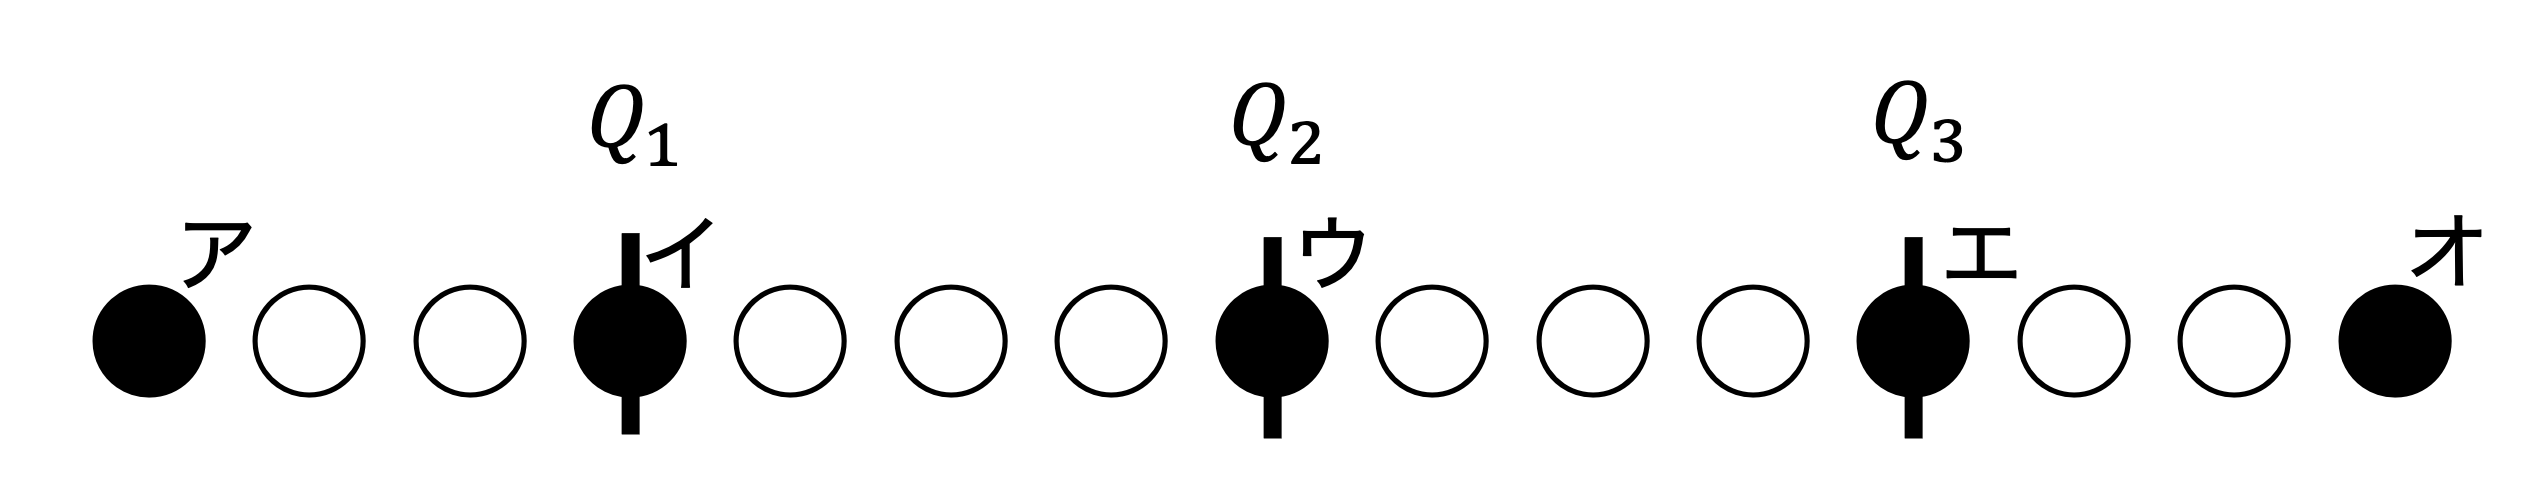
\includegraphics[width=10cm]{figure/5number.pdf}
	\caption{15個の量的データを小さい順に並べた例.}
	\label{fig:5number}
\end{figure}
%

%
五数要約の求め方はデータの数が奇数個の場合と偶数個の場合で異なる.
%
まず,データの数が奇数個の場合は最小値,最大値,中央値が自動的に定まる.
%
一方,中央値を除いて下位データと上位データに分けると,それぞれが偶数個になる.
%
この場合,下位データ,上位データそれぞれの中央にくる2つの値の平均値を第1四分位数,第3四分位数とする.
%

%
次に,データの数が偶数個の場合は中央にくる2つの値の平均値を中央値とする.
%
下位データと上位データはそれぞれ奇数個に分かれるので,第1四分位数,第3四分位数は自動的に求まる.
%

%
以下に具体例を示す.

\vspace{0.5cm}
\noindent 例)データが9個(奇数個)の場合
%
\begin{align*}
	2\ 3\ 5\ 5\ |\ 6\ |\ 8\ 10\ 12\ 15
\end{align*}
%
この場合,中央値は$ Q_{2}=6 $となるので,これを除いて下位データと上位データに分ける.
%
第1四分位数は$ Q_{1}=(3+5)/2=4 $,第3四分位数は$ Q_{3}=(10+12)/2=11 $と求まる.
%
四分位範囲は$ Q_{3}-Q_{1}=11-4=7 $である.
%

\vspace{0.5cm}
\noindent 例)データが10個(偶数個)の場合
%
\begin{align*}
	2\ 2\ 5\ 6\ 7\ |\ 9\ 10\ 13\ 14\ 18
\end{align*}
%
この場合,中央値は$ Q_{2}=(7+9)/2=8 $となる.
%
また,第1四分位数は$ Q_{1}=5 $,第3四分位数は$ Q_{3}=13 $と求まる.
%
四分位範囲は$ Q_{3}-Q_{1}=13-5=8 $である.


\subsubsection*{箱ひげ図}
%
五数要約の結果は図\ref{fig:boxplot}のような図によって可視化できる.
%
これを\textbf{箱ひげ図}と呼ぶ.
%
箱ひげ図は以下の手順によって描く(これを\textbf{テューキーの方式}と呼ぶ).
%
\begin{enumerate}
\item
データの第1四分位数から第3四分位数の間に箱を描く.
\item
中央値の位置に線を引く.
\item
箱から箱の長さ(四分位範囲)の1.5倍を超えて離れた点(外れ値)を白丸で描く.
\item
外れ値ではないものの最大値と最小値から箱まで線(ひげ)を引く.
\end{enumerate}
%
なお,外れ値を表示しない簡便な描き方もある.
%
また,90度回転させて横に描くことも多い.
%

%
\begin{figure}[H]
	\centering
	\includegraphics[width=8cm]{figure/boxplot.pdf}
	\caption{テューキーの方式による箱ひげ図の例.}
	\label{fig:boxplot}
\end{figure}
%

\subsubsection*{ヒストグラム}
%
データの分布の傾向(どの値がどのくらいあるか)を表す方法として,箱ひげ図ではデータを要約しすぎてしまい適切にその特徴を表せないことがある.
%
そこで,より詳細に分布の傾向を可視化する方法として度数分布表やそれを可視化した\textbf{ヒストグラム(度数分布図)}がある.
%
度数分布とは,値を0以上10未満,10以上20未満などのいくつかの区間(\textbf{階級},\textbf{ビン})に分けてそれぞれの区間に含まれるデータの個数(度数)をまとめたもので,横軸に階級の代表値(\textbf{階級値}),縦軸に度数をとったグラフがヒストグラムである.
%
なお,ヒストグラムの横軸には各階級の最小と最大を表示する場合と,階級値として階級の最小値や中央値を示す場合がある.
%
また,縦軸には度数ではなく相対度数(度数/データ数)を取ることもある.
%

%
%様々なデータについてヒストグラムを描くと,散らばり方も様々であることが分かる.
%
具体例として,ここではIris Dataset\footnote{Kaggleのウェブサイトからダウンロード可能:\url{https://www.kaggle.com/uciml/iris}}に含まれるアヤメのがく片の長さ,がく片の幅,花弁の長さ,花弁の幅のデータを用いる.
%
表\ref{tb:sepal_length_hist}はアヤメのがく片の長さのデータに対する度数分布表である.
%
ここでは,各階級の中央値を階級値としている.
%
また,度数,相対度数の他に,相対度数を足し合わせた累積度数も示している.
%

%
図\ref{fig:iris_hist}はアヤメのがく片の長さ,がく片の幅,花弁の長さ,花弁の幅のヒストグラムである.
%
ヒストグラムの中でデータが集中している部分が山のようになっているとき,山が1つの場合には単峰性,2つの場合には双峰性,それ以上の場合には多峰性と呼ぶ.
%
図\ref{fig:iris_hist}では,がく片のヒストグラムは単峰性,花弁のヒストグラムは双峰性である.
%
特に,多峰性のヒストグラムの場合には箱ひげ図によって可視化するとデータを要約しすぎてしまうため,適切にその特徴を表すことができない.
%
この他にも,値の小さなところにデータが集中していて大きな値のところに少数のデータがあるとき,「右に裾を引いている」という.
%

%
ヒストグラムの階級(ビン)の幅は大きすぎても細かすぎても分かりにくくなる.
%
一般に,階級数は標本の大きさ(サンプルサイズ)$ N $の平方根$ \sqrt{N} $程度が良いとされている.
%
例えば,100個のデータを含む場合は10程度の階級が望ましい.
%
また,$ 1 + \log_{2} N $という公式も存在し,これを\textbf{スタージェスの公式}と呼ぶ.
%
図\ref{fig:iris_hist}では,スタージェスの公式を用いて階級数を決めている.
%

%
\begin{table}[H]
    \centering
    \caption{アヤメのがく片の長さの度数分布表}
    \label{tb:sepal_length_hist}
    \scalebox{0.8}{
    \begin{tabular}{c|c|c|c|c|c}
    \hline
        最小(cm) & 最大(cm) & 階級値$ v_{i} $(cm) & 度数$ f_{i} $ & 相対度数(\%) & 累積相対度数(\%) \\ \hline
        4.30 & 4.75 & 4.53 & 11 & 7.3 & 7.3 \\ 
        4.75 & 5.20 & 4.97 & 30 & 20.0 & 27.3 \\ 
        5.20 & 5.65 & 5.43 & 24 & 16.0 & 43.3 \\ 
        5.65 & 6.10 & 5.88 & 24 & 16.0 & 59.3 \\ 
        6.10 & 6.55 & 6.32 & 31 & 20.7 & 80.0 \\ 
        6.55 & 7.00 & 6.78 & 17 & 11.3 & 91.3 \\ 
        7.00 & 7.45 & 7.22 & 7 & 4.7 & 96.0 \\ 
        7.45 & 7.90 & 7.68 & 6 & 4.0 & 100.0 \\ \hline
    \end{tabular}
    }
\end{table}
%

%
\begin{figure}[H]
	\centering
	\includegraphics[width=10cm]{figure/iris_hist.pdf}
	\caption{ヒストグラムの例.A:アヤメのがく片の長さ,B:がく片の幅,C:花弁の長さ,D:花弁の幅.}
	\label{fig:iris_hist}
\end{figure}
%

\subsection{実例:夏の避暑地の気候の特徴〜夏の避暑地が快適な理由は?}
%
日本への外国人旅行者は近年急増しているが,一方で,日本人の国内旅行者の動向を月別に見ると,表\ref{tb:travel}のように月ごとに変動している.
%
特に,5月や8月は国内旅行者の数が突出して多くなっているが,これはゴールデンウィークや夏休みを利用して旅行する人が多いからである.
%

\begin{itembox}[l]{実習}
%
表\ref{tb:travel}のデータから折れ線グラフを作成せよ.
%
\end{itembox}

\begin{table}[H]
\centering
\caption{2015年の月別国内旅行者数(観光庁「2015年旅行・観光消費動向調査」より)}
\label{tb:travel}
\scalebox{0.9}{
\begin{tabular}{c|cccccccccccc}
\hline
月    & 1    & 2    & 3    & 4    & 5    & 6    & 7    & 8    & 9    & 10   & 11   & 12   \\ \hline
旅行者数 & 4315 & 3620 & 5331 & 4456 & 6322 & 4693 & 4458 & 7177 & 5707 & 4647 & 4794 & 4952 \\ \hline
\end{tabular}
}
\end{table}

\subsubsection*{STEP 1:Problem}
%
ある高校に通う5人の高校生は,2015年の夏休みにそれぞれ別の都市で過ごした.
%
以下は日本の各都市についての気候に関する意見をまとめたものである.
%
\begin{itemize}
\item
軽井沢は東京と比べて過ごしやすかった
\item
東京も今年は涼しい日もあったけど,すごく暑い日が多かった
\item
熊谷は東京以上に暑かった
\item
沖縄は暑かったけど,慣れてしまえば逆に過ごしやすかった
\item
札幌は過ごしやすかったけど,大阪は東京と同じように暑かった
\end{itemize}
%
それぞれの場所で,本当に暑さに違いはあったのだろうか?
%
特に,日本では,夏に避暑地を訪れる人が多いが,避暑地にはどのような特徴があるのだろうか?
%

\subsubsection*{STEP 2:Plan}
%
気象庁のHP(\url{http://www.data.jma.go.jp/gmd/risk/obsdl/index.php})には1日の平均気温,最高気温,最低気温,湿度などのデータが掲載されている.
%
ここでは,1日の最高気温,最低気温,湿度のデータを収集する.
%

%
収集したデータは五数要約や箱ひげ図によって傾向を調べる.
%
また,夏の蒸し暑さを定量化した指標である\textbf{不快指数}を計算し,各都市の特徴を調べる.
%
不快指数は気温を$ t $,湿度を$ H $とすると
%
\begin{align}
	不快指数=0.81t + 0.01H(0.99t-14.3)+46.3
	\label{eq:hukai}
\end{align}
%
によって求められる.
%
一般に,不快指数が75になると人口の約1割が不快を感じ,85になると全員が不快になる(三省堂編集所,大辞林,三省堂(1988)).
%

\subsubsection*{STEP 3:Data}
%
\begin{itembox}[l]{実習}
%
\begin{itemize}
\item
気象庁のHPから2015年8月の各地点の1日の平均気温,最高気温,最低気温,湿度のデータ(csvファイル)をダウンロードせよ.
\item
ダウンロードしたデータをpythonなどで解析しやすいように加工せよ.
\end{itemize}
%
\end{itembox}

\subsubsection*{STEP 4:Analysis}
%
まず,最高気温に着目する.
%
収集したデータは,五数要約や箱ひげ図を使って特徴を整理することができる.
%

%
\begin{itembox}[l]{実習}
%
\begin{itemize}
\item
各都市の最高気温のデータに対し,五数要約と四分位範囲を求めよ.
\item 
五数要約の結果から,各都市に対して並行箱ひげ図を作成せよ.
\end{itemize}
%
\end{itembox}
%

%
\vspace{0.5cm}
%軽井沢や札幌は最高気温が低いため,涼しく感じることが多く避暑地として人気が高いことが分かった.
次に最低気温に着目する.
%
%最低気温について見ると,東京や大阪は変わらずに高いが,熊谷は昼間に比べて涼しくなる傾向がある.
%%
%最低気温で比較すると,本当に熊谷は東京や大阪と比べて過ごしやすいのだろうか?
%

\begin{itembox}[l]{実習}
%
%
\begin{itemize}
\item
各地点の最低気温のデータについて,並行箱ひげ図を作成せよ
\item
各地点について,熱帯夜(最低気温が25℃以上の夜)の日数を求めよ

\end{itemize}
%
\end{itembox}
%

%
\vspace{0.5cm}
最後に不快指数に着目する.
%
\begin{itembox}[l]{実習}
%
\begin{itemize}
\item
式\eqref{eq:hukai}を用いて,6地点の2015年8月1日から31日までの不快指数を計算せよ
\item
各地点の不快指数のデータについて,並行箱ひげ図を作成せよ
\end{itemize}
%
\end{itembox}
%

\subsubsection*{STEP 5: Conclusion}
%
解析の結果を基に,各都市の気候についてどのようなことが分かるか考察する.
%

\begin{itembox}[l]{実習}
%
\begin{itemize}
\item
最高気温に対する並行箱ひげ図を基に,各地点の特徴について分かったことを次の観点からまとめよ.
	%
	\begin{enumerate}
	\item
	東京や大阪のような大都市は避暑地と比べて暑い日が多いか?
	\item
	避暑地として人気の高い軽井沢は高原にあるが,北海道とどのように違うか?
	\item
	熊谷や沖縄は暑い地域として有名だが,それぞれで違いはあるか?	 
	\end{enumerate}
	%
\item
熊谷は最高気温は高いが,最低気温は東京や大阪と比べて低い.なぜこのような違いが出るのか考えよ.
\item
不快指数を基に,各都市の特徴をまとめよ
\item
軽井沢や札幌は夏の避暑地として人気が高い.その理由をまとめよ.
\item
その他,分析結果を元に自由に考察せよ.
\end{itemize}
%
\end{itembox}


\clearpage
\section{特性値の活用}
%
データの性質を定量的に表すための統計量(データに対して何らかの統計的な計算をして得られた数値)を\textbf{特性値}という.
%
代表値,記述統計量,要約統計量などとも呼ばれる.
%
ここでは代表的な特性値について説明する.
%
なお,以下では$ n $個のデータを$ (x_{1}, x_{2}, \cdots, x_{n}) $と表す.

\subsection{データの中心を表す特性値}

\subsubsection*{算術平均}
%
データの中心を表す特性値として最もよく知られ,よく用いられるのが\textbf{算術平均}であり,
%
\begin{align}
	\bar{x} &= \frac{x_{1}+x_{2}+\cdots+x_{n}}{n} = \frac{1}{n} \sum_{i=1}^{n}x_{i}
	\label{eq:arithmetic_mean}
\end{align}
%
と定義される.
%
通常,与えられたデータから平均値を求めるにはこの式に当てはめれば良い.
%
例えば,アヤメのがく片の長さのデータの場合,平均値は$ \bar{x}=5.843 $ cmとなる.
%
算術平均は分布形状が左右対称に近いデータの場合にはデータの中心を表す量と捉えられるが,分布形状が極端に非対称な場合にはデータの中心を表す特性値としてふさわしくない.
%

%
算術平均は度数分布表から求めることもできる.
%
具体的には,階級値を$ v_{i} $,対応する度数を$ f_{i} $,階級の数を$ k $とすると,平均値は
%
\begin{align}
	\bar{x} &= \frac{f_{1}v_{1}+f_{2}v_{2}+\cdots+f_{k}v_{k}}{f_{1}+f_{2}+\cdots+f_{k}}
	= \frac{1}{n} \sum_{i=1}^{k} f_{i}v_{i}
	\label{eq:arithmetic_mean2}
\end{align}
%
と表される.
%
例えば,アヤメのがく片の長さのデータ(表\ref{tb:sepal_length_hist})の場合,
%
\footnotesize
\begin{align*}
	\bar{x} &= \frac{4.53\times11+4.97\times30+5.43\times24+5.88\times24+6.33\times31+6.78\times17+7.22\times7+7.68\times6}{11+30+34+34+31+17+7+6}\\
	&= 5.854
\end{align*}
\normalsize
%
となる.
%

%
以上の例を見て分かるように,度数分布表から求めた平均値はデータから直接求めた平均値と一致しない.
%
これは,度数分布表から求めた平均値が近似値であるからである.
%
度数分布表では,各階級の値を階級値で代表させているためこのようなことが起こるが,各階級の幅を十分小さく取れば近似の度合いは上昇する.
%

%%
%\begin{table}[H]
%    \centering
%    \caption{度数分布表から平均・分散を求める例}
%    \label{tb:ex_mean_hist}
%    \scalebox{0.8}{
%    \begin{tabular}{c|c|c|c|c|c}
%    \hline
%        最小 & 最大 & 階級値$ v_{i} $ & 度数$ f_{i} $ & $ f_{i}v_{i} $ & $ f_{i}(v_{i}-\bar{x})^{2} $ \\ \hline
%        0  & 10 & 5  & 12 & 60 & 28979.3 \\ 
%        10 & 20 & 15 & 10 & 150 & 15321.0 \\ 
%        20 & 30 & 25 & 19 & 475 & 16136.0 \\ 
%        30 & 40 & 35 & 42 & 1470 & 15389.6 \\ 
%        40 & 50 & 45 & 72 & 3240 & 6017.6 \\ 
%        50 & 60 & 55 & 82 & 4510 & 60.4 \\ 
%        60 & 70 & 65 & 54 & 3510 & 6366.3 \\ 
%        70 & 80 & 75 & 38 & 2850 & 16532.0 \\
%        80 & 90 & 85 & 25 & 2125 & 23805.3 \\ 
%        90 & 100 & 95 & 19 & 1805 & 31718.0 \\\hline
%         & 合計 &  & 373 & 20195 & 160325.5 \\\hline
%    \end{tabular}
%    }
%\end{table}
%%

\subsubsection*{幾何平均(相乗平均)}
%
算術平均に対して,幾何平均というものも存在する.
%
これは,$ n $個のデータに対して,値の積の$ n $乗根をとったもので,
%
\begin{align}
	\bar{x}_{g} &= \sqrt[n]{x_{1}\times\cdots \times x_{n}} = \sqrt[n]{\prod_{i=1}^{n}x_{i}} = \left(\prod_{i=1}^{n}x_{i}\right)^{1/n}
	\label{eq:geometric_mean}
\end{align}
%
と定義される.
%
定義より,幾何平均は正の数のみしか扱えず,さらに掛け算によって定義されるので比率データにしか適用できない.
%

%
幾何平均は成長率や倍率の平均を計算するときに用いられる.
%
例えば,次のような事例を考える:
%
\begin{quotation}
1年目から2年目にかけての物価は対前年比2倍になり(100円のものが200円になり),2年目から3年目にかけての物価は対前年比8倍となった(200円のものが1600円になった).
では,この2年間の物価の対前年比伸び率の平均はいくらか?
\end{quotation}
%
まず,算術平均を適用してみる.
%
すると,物価の対前年比伸び率の平均は$ (2+8)/2=5 $倍となる.
%
これは,1年目に100円だったものが2年目に500円になり,さらに3年目に2500円になることを意味するので,実際よりも過大に見積もってしまう.
%
そこで,次に幾何平均を適用してみる.
%
すると,物価の対前年比伸び率の平均は$ \sqrt[2]{2\times 8}=4 $倍となる.
%
これは,1年目に100円だったものが2年目に400円になり,さらに3年目に1600円になることを意味するので,実際の金額と一致する.
%
このように,倍率の平均値を計算する場合には,算術平均ではなく幾何平均を用いるのが妥当である.
%

\subsubsection*{中央値・最頻値}
%
データの分布形状が歪んでいる場合,算術平均はデータの中心を表す特性値としてふさわしくない.
%
例えば,
%
\begin{align*}
	1,1,1,1,2,3,4,5,16,20 
\end{align*}
%
のようなデータがあったとき,この算術平均は5.4になるが,平均より小さいものが8個を占め,残りの2個が平均より大きい.
%
これは,少数のデータ(16と20)が平均を押し上げている例である.
%
このような場合,分布の中心という意味では既に述べた\textbf{中央値(メディアン)}を用いる方が適切である.
%
実際,中央値を用いれば,その値より小さい数と大きい数の個数が等しくなる.
%

%
平均値,中央値の他によく用いられる特性値として,\textbf{最頻値(モード)}がある.
%
これは,データの中で最も頻出する数であり,度数分布表において度数が最大となる階級の階級値に対応する.
%
ただし,分布形状が双峰性の場合には有効な特性値とならないので注意が必要である.
%

\subsection{データのばらつきを表す特性値}
%
データの特性を知りたい場合,中心を表す特性値だけでは情報不足であり,中心からどの程度ばらついているかも考慮しなければならない.
%
例えば,以下の3つのデータは中心を表す算術平均,中央値,最頻値がすべて5であるが,分布の形状は異なる.
%
\begin{align*}
	&A: 0,3,3,5,5,5,5,7,7,10 \\
	&B: 0,1,2,3,5,5,7,8,9,10 \\
	&C: 3,4,4,5,5,5,5,6,6,7
\end{align*}
%

%
通常,ばらつきを求める際には,算術平均からの距離$ x_{i} - \bar{x} $を考える.
%
これを\textbf{偏差}と呼ぶ.
%
この偏差を全データに対して平均すれば,ばらつきを表す特性値になりそうであるが,これだと問題が生じる.
%
例えば,データが左右対称に分布している場合,平均より小さい値のデータ(偏差が負)と大きい値のデータ(偏差が正)が同程度あるため,偏差を平均するとほぼ0になってしまう.
%
ばらつきが0というのは明らかにおかしいため,別の特性値を考える必要がある.
%
以下に代表的な方法を示す.
%

\subsubsection*{平均偏差}
%
1つ目の方法は偏差の絶対値を取ってから平均するというものであり,\textbf{平均偏差}と呼ばれる:
%
\begin{align}
	平均偏差 &= \frac{1}{n} \sum_{i=1}^{n}|x_{i}-\bar{x}| 
	\label{eq:mean_deviation}
\end{align}
%
%これは,分布の中心を平均$ \bar{x} $として,そこから平均的にどれだけ離れているかを表した量である.
%
これは,$ n $個のデータの1個当りの平均からの距離であり,ばらつきの指標として直感的に理解しやすい.
%
しかし,絶対値の扱いが数学的に面倒,分布の中心が$ \bar{x} $ではなく中央値のときに最小になる,平均から大きく外れた値も等しい寄与となる,など問題があるため利用されることは少ない.
%

\subsubsection*{分散・標準偏差}
%
2つ目の方法は,偏差の2乗をとってから平均するというものであり,\textbf{分散}と呼ばれる:
%
\begin{align}
	s^{2} &= \frac{1}{n} \sum_{i=1}^{n} (x_{i} - \bar{x})^{2}
	\label{eq:deviation}
\end{align}
%
分散は$ n $個のデータ1個当りの平均からの距離の2乗であり,平均から大きく離れるほど寄与が大きくなる指標である.
%
%特に,平均偏差と対照的に,分布の中心が$ \bar{x} $のときに最小となる.
%
また,分散の平方根$ s $は\textbf{標準偏差}と呼ばれる:
%
\begin{align}
	s &= \sqrt{\frac{1}{n} \sum_{i=1}^{n} (x_{i} - \bar{x})^{2}}
	\label{eq:standard_deviation}
\end{align}
%
標準偏差はデータの測定単位と同一の単位となるので扱いやすい.
%
通常,データのばらつきを表す特性値としては分散または標準偏差が最もよく用いられる.
%

%
なお,平均と同様に分散・標準偏差を度数分布から求めることもできる:
%
\begin{align}
	\begin{split}
	s^{2} &= \frac{1}{n} \sum_{i=1}^{k} (v_{i} - \bar{x})^{2} f_{i} \\
	s &= \sqrt{\frac{1}{n} \sum_{i=1}^{k} (v_{i} - \bar{x})^{2} f_{i}}
	\end{split}
	\label{eq:deviation2}
\end{align}
%

\subsubsection*{変動係数}
%
標準偏差は測定単位によって値が変化してしまう.
%
また,データの水準の変化(おおまかには平均値の大きさ)とともに標準偏差の大きさは変化する.
%
そこで,データの水準を平均値によって調整した指標が変動係数(Coefficient of Variation)で,次式で定義される:
%
\begin{align}
	\mathrm{CV} &= \frac{s}{\bar{x}}
	\label{eq:cv}
\end{align}
%
変動係数は同じ単位を持つ量同士で割り算をしているので,無次元(単位がない)となり,データの測定単位に寄らない.
%
通常,単位や平均が異なるグループ間でばらつきを比較する際には変動係数が用いられる.
%

%\subsection{その他の特性値}
%
%\subsubsection*{歪度}
%%
%平均,分散とともに分布の形状を表す指標が歪度,尖度である.
%%
%まず,\textbf{歪度}は
%%
%\begin{align*}
%	歪度 &= \frac{1}{n} \sum_{i=1}^{n} \left( \frac{x_{i}-\bar{x}}{s}\right)^{3}
%\end{align*}
%%
%と定義される.
%%
%歪度は左右対称な分布では0となり,右に歪んだ分布では正,左に歪んだ分布では負となる.
%%
%
%\subsubsection*{尖度}
%%
%\textbf{尖度}は
%%
%\begin{align*}
%	尖度 &= \frac{1}{n} \sum_{i=1}^{n} \left(\frac{x_{i}-\bar{x}}{s}\right)^{4}
%\end{align*}
%%
%と定義される.
%%
%正規分布では尖度は3となり,3より大きな値をとる分布では正規分布よりも中心が尖っていて,裾が厚くなる傾向がある.
%%
%
%\subsubsection*{積率}
%%
%次式で定義される量
%%
%\begin{align*}
%	m_{k} &= \frac{1}{n} \sum_{i=1}^{n} x_{i}^{k}
%\end{align*}
%%
%を\textbf{$ k $次の積率(モーメント)}という.
%%
%平均,分散,歪度,尖度はそれぞれ1次,2次,3次,4次のモーメントの情報を反映した量である.
%%

\subsection{ローレンツ曲線とジニ係数}
%
%\textbf{ローレンツ曲線}は,社会の構成員を所得の小さい順に並べて$ n $個の階級に分け,横軸に構成員の累積相対度数,縦軸に所得の累積相対度数を取ったグラフである.
%
ある社会を構成する構成員(人物でも市町村でも何でも良い)に対し,所得が対応したデータを考える.
%
この構成員を所得の小さい順に並べて$ n $個の階級に分け,階級$ i $のサイズ(人数や個数)を$ x_{i} $,平均所得を$ y_{i} $とする.
%
また,サイズの累積相対度数を$ X_{i} $,平均所得の累積相対度数を$ Y_{i} $とする.
%
このとき,横軸に構成員の累積相対度数,縦軸に所得の累積相対度数を取ったグラフを\textbf{ローレンツ曲線}と呼ぶ.
%
グラフの横軸,縦軸はともに0から1の範囲であり,曲線上の$ (X, Y) $という点は,社会全体の貧しい側から$ X\times100 $\%の人が全体の$ Y\times100 $\%の富を占めることを表す.
%
例えば,$ (0.25, 0.1) $という点は,社会全体の25\%の人が10\%の富を占めるということを表す.
%
ローレンツ曲線はこれらの点を点線で結んだ折れ線グラフとして表され,必ず両端が$ (0, 0) $と$ (1, 1) $になる.
%
もし,富が全構成員に平等に配分されている場合,ローレンツ曲線は傾き1の直線となり,これを\textbf{完全平等線}と呼ぶ.
%
一方,富の配分に格差があるほどローレンツ曲線は完全平等線から下にずれていく.
%
このように,ローレンツ曲線はある社会における富の配分格差を可視化したグラフといえる.
%

%
社会の格差の度合いはローレンツ曲線が完全平等線から下にずれるほど大きくなる.
%
よって,ローレンツ曲線と完全平等線によって囲まれた部分の面積が,完全平等線,$ x=1 $,$ y=0 $で構成される三角形の面積に占める割合を格差の指標と考えることができる.
%
この指標は\textbf{ジニ係数}と呼ばれる.
%
階級を$ n $等分したとき,下から$ i $番目の階級の平均所得を$ y_{i} $とする($ y_{1}\leq y_{2} \leq \cdots \leq y_{n} $).
%
このとき,ジニ係数を以下のように表すこともできる:
%
\begin{align}
	G &= \frac{1}{2n^{2} \bar{y}} \sum_{i=1}^{n} \sum_{j=1}^{n} |y_{i} - y_{j}|
	\label{eq:gini}
\end{align}
%
ただし,$ \bar{y} = \frac{1}{n} \sum_{i=1}^{n} y_{i} $は全体の平均所得である.
%
ジニ係数は0から1の間で定義され,完全に平等な配分のときに$ G=0 $,一人がすべての所得を占有しているときに$ G=(n-1)/n $となる(つまり$ n $が大きいときには1に近づく).
%

%
例として,$ n=3 $の場合を考える.
%
まず,式\eqref{eq:gini}を用いてジニ係数を計算すると,
%
\begin{align*}
	\sum_{i=1}^{3}\sum_{j=1}^{3} |y_{i}-y_{j}|
	&= 2\{(y_{2}-y_{1})+(y_{3}-y_{1})+(y_{3}-y_{2})\} \\
	&= 4(y_{3}-y_{1}) \\
	\bar{y} &= \frac{1}{3} (y_{1}+y_{2}+y_{3})
\end{align*}
%
より
%
\begin{align*}
	G &= \frac{2}{3} \frac{y_{3}-y_{1}}{y_{1}+y_{2}+y_{3}}
\end{align*}
%
となる.
%

%
次に,面積からジニ係数を計算する.
%
横軸と縦軸の値はそれぞれ表\ref{tb:lorentz}のようになる.
%
ローレンツ曲線と$ x=1 $,$ y=0 $に囲まれた領域の面積は1つの三角形と2つの台形から成るので,
%
\begin{align*}
	\frac{1}{2}\cdot\frac{1}{3} \left[\alpha_{1}+(\alpha_{1}+\alpha_{2})+(\alpha_{2}+1)\right]
	&= \frac{1}{6}(2\alpha_{1}+2\alpha_{2}+1)
\end{align*}
%
これより,完全平等線と$ x=1 $,$ y=0 $に囲まれた領域の面積は
%
\begin{align*}
	\frac{1}{2} - \frac{1}{6}(2\alpha_{1}+2\alpha_{2}+1) = \frac{1}{3} (1-\alpha_{1}-\alpha_{2})
\end{align*}
%
となるので,ジニ係数は
%
\begin{align*}
	G = \frac{1}{3} (1-\alpha_{1}-\alpha_{2}) \div \frac{1}{2} &= \frac{2}{3} (1-\alpha_{1}-\alpha_{2}) = \frac{2}{3} \frac{y_{3}-y_{1}}{y_{1}+y_{2}+y_{3}}
\end{align*}
%
と求まる.
%

%
以上より,式\eqref{eq:gini}から求めたジニ係数と面積から求めたジニ係数が確かに一致することが分かった.
%
なお,一般の$ n $に対する証明は省略する.
%

\begin{table}[H]
\centering
\caption{$ n=3 $の場合の度数分布表}
\label{tb:lorentz}
\scalebox{0.8}{
\begin{tabular}{c|c|ccc}
\hline
\multirow{2}{*}{階級} & \multicolumn{1}{c|}{横軸(構成員)} & \multicolumn{3}{c}{縦軸(所得)}  \\ \cline{2-5}
                     & 累積相対度数             & 平均所得$ y $ & 累積度数$ Y $ & 累積相対度数 \\ \hline
I                    & 1/3     & $ y_{1} $   & $ y_{1} $   & $ \alpha_{1}=\frac{y_{1}}{y_{1}+y_{2}+y_{3}} $ \\
II                   & 2/3     & $ y_{2} $   & $ y_{1}+y_{2} $   & $ \alpha_{2}=\frac{y_{1}+y_{2}}{y_{1}+y_{2}+y_{3}} $  \\
III                  & 1       & $ y_{3} $  & $ y_{1}+y_{2}+y_{3} $  & 1  \\ \hline
\end{tabular}
}
\end{table}

\begin{table}[H]
\centering
\caption{ローレンツ曲線作成のためのサンプルデータ}
\label{tb:lorentz2}
\scalebox{0.8}{
\begin{tabular}{c|ccc|ccc}
\hline
\multirow{2}{*}{階級} & \multicolumn{3}{c|}{横軸(構成員)}      & \multicolumn{3}{c}{縦軸(所得)} \\ \cline{2-7}
  & 人数$ x $ & 累積度数$ X $ & 累積相対度数 & 平均所得$ y $ & 累積度数$ Y $ & 累積相対度数 \\ \hline
I   & 25 & 25   & 0.25         & 15     & 15       & 0.0937       \\
II  & 25 & 50   & 0.5         & 25     & 40       & 0.25         \\
III & 25 & 75   & 0.75         & 40     & 80       & 0.5         \\
IV  & 25 & 100  & 1        & 80     & 160      & 1        \\ \hline
\end{tabular}
}
\end{table}

%
\begin{figure}[H]
	\centering
	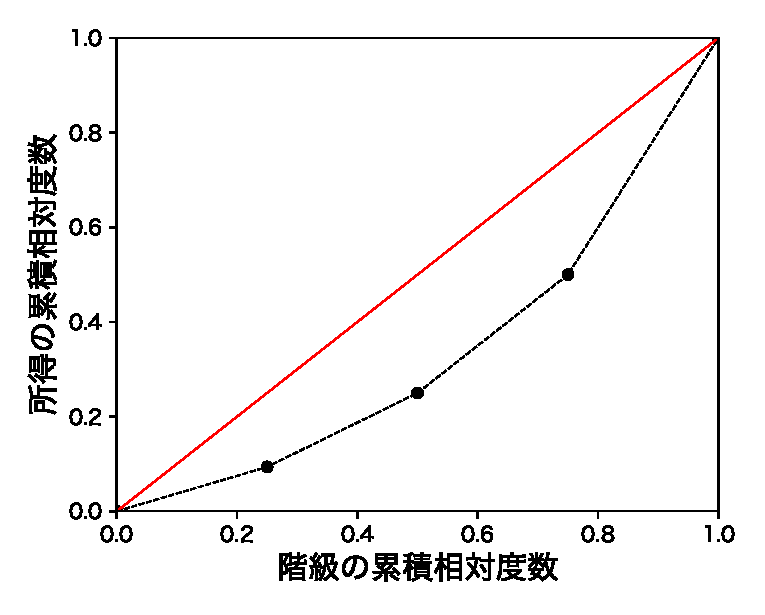
\includegraphics[width=8cm]{figure/lorentz.pdf}
	\caption{ローレンツ曲線の例(表\ref{tb:lorentz2}から作成)}
	\label{fig:lorentz}
\end{figure}
%


\subsection{実例:地域の豊かさの格差は拡大しているか?}
%

\subsubsection*{STEP 1: Problem}
%
2015年の国勢調査では,日本全体の人口が1920年の調査開始以来,初めて減少したことが明らかになった.
%
また,都道府県ごとの人口を見ても,5年前(2010年)に比べて人口が減少したのは39の道府県にのぼる.
%
一方,東京を中心とした大都市には人口が集中し,都市部と地方の格差が広がっているのも事実である.
%
人口は経済・社会の基盤を成すものであり,人口の増減は経済的な豊かさと密接に関わっていると思われる.
%
近年の人口変動によって,地域間で経済的な豊かさの格差は拡大したのだろうか?
%

\subsubsection*{STEP 2: Plan}
%
地域ごとの経済的な豊かさを捉える指標として,\textbf{都道府県別の1人当たり県民所得}に着目する.
%
これは,企業を含めて県民全体の経済水準を表すもので,都道府県間で比較可能な統計データである.
%
ただし,各都道府県は人口規模が大きく異なるので,地域ごとに比較する際には規模を表す人口等の変数で除した量を用いることが必要となる.
%
そこで,今回用いる1人当たり県民所得は,県民所得を県内に居住する人口(「国勢調査」と「人口推計」に準拠)で除して求める.
%
また,格差の大きさは一人当たり県民所得の標準偏差,変動係数,ジニ係数で評価し,ばらつきが40年間で拡大しているか否かを調べる.
%

\subsubsection*{STEP 3: Data}
%
1人当たり県民所得は,内閣府「県民経済計算」(\url{https://www.esri.cao.go.jp/jp/sna/data/data_list/kenmin/files/files_kenmin.html})から利用することができる.
%
ただし,年度が同じでも基準(平成23年基準や平成17年基準など)によって算出された値が異なることに注意する.
%
%例として,表\ref{tb:income}に2013年度の1人当たり県民所得を都道府県別に示す.
%
%また,各都道府県の人口は「国勢調査」(総務省)に拠っている.
%

%\begin{table}[H]
%    \centering
%    \caption{2013年度1人当たり県民所得(万円)}
%    \label{tb:income}
%    \begin{tabular}{|lll|lll|lll|}
%    \hline
%        01 & 沖縄県 & 210 & 17 & 岩手県 & 270 & 33 & 石川県 & 297 \\ 
%        02 & 鳥取県 & 234 & 18 & 長野県 & 271 & 34 & 京都府 & 297 \\ 
%        03 & 鹿児島県 & 240 & 19 & 岐阜県 & 273 & 35 & 大阪府 & 300 \\ 
%        04 & 宮崎県 & 241 & 20 & 新潟県 & 277 & 36 & 千葉県 & 302 \\ 
%        05 & 島根県 & 242 & 21 & 福島県 & 279 & 37 & 群馬県 & 305 \\ 
%        06 & 長崎県 & 242 & 22 & 岡山県 & 280 & 38 & 広島県 & 306 \\ 
%        07 & 熊本県 & 242 & 23 & 香川県 & 280 & 39 & 山口県 & 312 \\ 
%        08 & 青森県 & 243 & 24 & 兵庫県 & 282 & 40 & 茨城県 & 314 \\ 
%        09 & 高知県 & 245 & 25 & 和歌山県 & 282 & 41 & 富山県 & 316 \\ 
%        10 & 秋田県 & 246 & 26 & 福岡県 & 283 & 42 & 三重県 & 317 \\ 
%        11 & 佐賀県 &  251 & 27 & 福井県 & 285 & 43 & 栃木県 & 325 \\ 
%        12 & 奈良県 &  253 & 28 & 宮城県 & 286 & 44 & 滋賀県 & 327 \\ 
%        13 & 愛媛県 &  254 & 29 & 埼玉県 & 286 & 45 & 静岡県 & 333 \\ 
%        14 & 北海道 &  255 & 30 & 徳島県 & 288 & 46 & 愛知県 & 358 \\ 
%        15 & 大分県 &  256 & 31 & 山梨県 & 292 & 47 & 東京都 & 451 \\ \cline{7-9}
%        16 & 山形県 &  263 & 32 & 神奈川県 & 297 &  & 全県平均 & 307 \\ \hline
%    \end{tabular}
%\end{table}

\subsubsection*{STEP 4: Analysis}
%
まず,1人当たりの県民所得の平均と標準偏差に着目する.
%

%
\begin{itembox}[l]{実習}
%
\begin{itemize}
\item
1975年から2018年までの1人あたり県民所得のcsvファイルを読み込み,各年度に対して平均と標準偏差を求めよ.
\item
1975年〜91年の標準偏差は一貫して増加しており,格差は拡大しているように見えるが,本当にそう言えるか?平均値の変化と関連付けて考えよ.
\end{itemize}
%
\end{itembox}
%

%図\ref{fig:income_mean_sd}の左軸は1人当たり県民所得の平均の年次変化,右軸は標準偏差の年次変化(いずれも1975年〜2013年まで)を表している.
%%
%この図から,1975年〜91年の標準偏差は一貫して増加しており,格差は拡大しているように見える.
%%
%しかし,この期間は平均も標準偏差と同様の増加傾向を示している.
%%
%つまり,経済成長に伴って所得の平均が増加した結果,標準偏差も大きくなったと考えるのが妥当である.
%%
%これは,例えば,$ Y_{i} $が円単位の場合と万円単位の場合にそれぞれ標準偏差を計算すると,前者の標準偏差は後者の場合の1万倍になることからも分かる.
%%
%%つまり,各時点間での標準偏差を比較するには,各時点での所得水準(平均)を調整した指標を用いなければならない.
%

%
\vspace{0.5cm}
次に,標準偏差を平均で割った変動係数の変化を調べる.

%
\begin{itembox}[l]{実習}
%
\begin{itemize}
\item
全年度に対して変動係数を求め,時系列変化を可視化せよ.
\item
変動係数の変化から,1975年〜91年および全期間にかけて格差が増加しているか考えよ.
\end{itemize}
%
\end{itembox}
%

%%
%図\ref{fig:income_sd_cv}は標準偏差のグラフに変動係数のグラフを重ねて表したものである.
%%
%このグラフから,変動係数の値は1975年〜91年においてほぼ一定になっていることが分かる.
%%
%また,全期間を通しても,1975年は0.16,2013年は0.15なので,ほぼ同様な水準にある.
%%

%
\vspace{0.5cm}
次に,所得格差を表すジニ係数に着目する.
%

%
\begin{itembox}[l]{実習}
%
\begin{itemize}
\item
年度を1つ選び,その年度のローレンツ曲線とジニ係数を求めよ.
\item
全年度に対してジニ係数を求め,時系列変化を可視化せよ.
\item
ジニ係数の変化から,1975年〜91年および全期間にかけて格差が増加しているか考えよ.
\end{itemize}
%
\end{itembox}
%

%%
%図\ref{fig:income_sd_gini}は変動係数のグラフにジニ係数のグラフを重ねて表したものである.
%%
%このグラフから,ジニ係数は変動係数とほぼ同じ変動を示しており,いずれの場合も2013年度に至る約40年で都道府県間の所得格差が拡大しているとは読み取れない.
%%


\subsubsection*{STEP 5: Conclusion}
%
解析の結果を元に,1975年からの40年間で格差が増加したのかどうか考察する.
%

%
\begin{itembox}[l]{実習}
%
\begin{itemize}
\item
格差を表す指標の40年間の推移から地域間で経済的な豊かさの格差が拡大したのかどうか考えよ.
\item
格差を表す指標の40年間の推移を見ると,細かい時間スケールでの変動が見られる.これらは具体的にどのような出来事を反映していると考えられるか?
\end{itemize}
%
\end{itembox}
%

%%
%変動係数やジニ係数の約40年間の推移を見る限り,地域間で経済的な豊かさの格差が拡大したとはいえない.
%%
%ただし,1980年代後半のバブル期に至る時期にかけてやや格差が拡大した.
%%
%その後の景気低迷の中で,景気対策としての地方への公共事業の重点配分などの結果,地域間格差は低下した.
%%
%しかし,景気対策の後遺症として,国と地方の財政赤字は膨れ上がり,小泉政権下での公共事業抑制や行政改革への転換に伴って地域間格差は再び拡大した.
%%
%その後の政策転換と2008年9月のリーマンショック後の世界不況のもとで地域間格差は縮小し,現在に至る.
%%

\clearpage
\section{関係の度合い}

\subsection{散布図と相関係数}
%
ここまでは1種類の量的データの要約法を扱ってきたが,一方で2種類の量的データの間の関係について知りたい場合もある.
%
ここでは,2種類の量的データを変数$ X $と$ Y $で表し,これらの間の関係を可視化・定量化する方法を扱う.
%

%
まず,2つの量的データの間の関係を可視化するには,それぞれを横軸と縦軸に取ったグラフを描けば一目瞭然である.
%
このようなグラフは\textbf{散布図}と呼ばれる.
%
より具体的に散布図とは,$ n $組のデータ$ (x_{1}, y_{1}),\ (x_{2}, y_{2}), \ldots, (x_{n}, y_{n}) $に対し,$ (x_{i}, y_{i}) $を座標とする点を$ X-Y $平面上にとったグラフのことである.
%
なお,データは必ず点でプロットし,データ同士を線で結んだりはしない.
%
例として,アヤメデータについて,がく片の長さと幅,花弁の長さと幅の散布図を図\ref{fig:scatter_iris}に示す.
%
まず,がく片の散布図を見ると,長さに対して幅が一定となっており,特に2つの変数に関係はないようである.
%
一方,花弁については右上と左下の区画にデータ点が多く,右上がりの傾向がある.
%
すなわち,花弁が長くなれば,それとともに花弁の幅も大きくなる傾向がある.
%

%
なお,もし散布図の中に他の点から極端に外れた点がある場合は外れ値の可能性が高い.
%
このような場合には加工に誤りがないか調べ,データ解析からその値を削除するかどうか検討する.
%

%
\begin{figure}[H]
	\centering
	\includegraphics[width=12cm]{figure/scatter_iris.pdf}
	\caption{A:アヤメのがく片の長さと幅の散布図.B:アヤメの花弁の長さと幅の散布図.}
	\label{fig:scatter_iris}
\end{figure}
%

%%
%\begin{table}[H]
%    \centering
%    \caption{日最高気温と飲料支出金額}
%    \label{tb:scatter_ex}
%    \begin{tabular}{l|llllll}
%    \hline
%        月 & 1 & 2 & 3 & 4 & 5 & 6 \\ \hline
%        日最高気温(℃) & 9.1 & 10.2 & 14.1 & 19.8 & 25.0 & 26.8 \\ 
%        飲料支出金額(円) & 3416 & 3549 & 4639 & 3857 & 3989 & 4837 \\ \hline
%    \end{tabular}
%    \begin{tabular}{l|llllll}
%    \hline
%        月 & 7 & 8 & 9 & 10 & 11 & 12 \\ \hline
%        日最高気温(℃) & 31.1 & 34.0 & 28.5 & 22.9 & 15.7 & 11.3 \\ 
%        飲料支出金額(円) & 5419 & 5548 & 4311 & 4692 & 3607 & 4002 \\ \hline
%    \end{tabular}
%\end{table}
%%
%
%%
%\begin{figure}[H]
%	\centering
%	\includegraphics[width=6cm]{figure/scatter_ex.pdf}
%	\caption{日最高気温と飲料支出金額の散布図}
%	\label{fig:scatter_ex}
%\end{figure}
%%

%
変数$ X,\ Y $の散布図に右上がりの傾向などがある場合には相関関係があるという.
%
このような相関関係を定量化した量は\textbf{ピアソンの相関係数}と呼ばれ,以下の式で定義される:
%
\begin{align}
	r_{XY} &= \frac{\displaystyle\frac{1}{n} \sum_{i=1}^{n}(x_{i}-\bar{x})(y_{i}-\bar{y})}{\displaystyle\sqrt{\frac{1}{n} \sum_{i=1}^{n}(x_{i}-\bar{x})^{2}}\sqrt{\frac{1}{n} \sum_{i=1}^{n}(y_{i}-\bar{y})^{2}}} = \frac{s_{XY}}{s_{X}s_{Y}}
	\label{eq:correlation}
\end{align}
%
また,分散公式を用いると,
%
\begin{align}
	r_{XY} &= \frac{\overline{xy} - \bar{x}\bar{y}}{(\overline{x^{2}} - \bar{x}^{2})(\overline{y^{2}} - \bar{y}^{2})}
	\label{eq:correlation2}
\end{align}
%
と表すこともできる.
%
ここで,式\eqref{eq:correlation}の分子に現れた量
%
\begin{align}
	s_{XY} &= \frac{1}{n} \sum_{i=1}^{n}(x_{i}-\bar{x})(y_{i}-\bar{y}) = \overline{xy} - \bar{x}\bar{y}
	\label{eq:covariance}
\end{align}
%
は変数$ X,\ Y $の\textbf{共分散}と呼ばれる($ \mathrm{Cov}(X, Y) $と表すこともある).
%
共分散は各データごとに$ X,\ Y $の偏差(平均との差)の積を考え,それらの全データに対する平均を考えている.
%
これにより,散布図が右上がりのときに正,右下がりのときには負となる統計量が得られる.
%
ただし,これだけだと$ X,\ Y $の単位やばらつきの度合いによって値が大きく異なってしまい,相関の程度を一定の基準で表すことができない.
%
そこで,共分散を$ X,\ Y $の標準偏差で割って,各変数の単位やばらつきの度合いに依らない量としたのが相関係数である.
%

%
実際,相関係数の定義域は$ -1\leq r_{XY} \leq 1 $であり,その絶対値によって相関の強さを表すことができる.
%
また,定義より,相関係数の符号は右上がりの傾向の場合に正,右下がりの傾向の場合に負となる.
%
特に,相関係数が正の値のときに\textbf{正の相関},負の値のときに\textbf{負の相関}があるという.
%
また,相関係数が0のときには\textbf{無相関}という.
%
実際に図\ref{fig:scatter_iris}から相関係数を求めると,がく片については$ r_{XY} = -0.11 $なのでほぼ無相関,花弁については$ r_{XY}=0.96 $となるので強い正の相関があることが分かる.
%

%
なお,相関係数はあくまでも2つの変数の散布図が直線的な関係になる場合だけ意味があることに注意しなければならない.
%
例えば,$ X,\ Y $の散布図が円状に分布する場合,2つの変数には何かしらの規則があると考えられるが,相関係数は0となり無相関と判断されてしまう.
%
このため,相関係数を調べる際には必ず散布図も併せて描く必要がある.
%

\subsection{相関関係と因果関係}
%
2つの変数$ X,\ Y $の間に相関関係があったときに,それらの間に因果関係があるといえるだろうか?
%
つまり,$ X\Rightarrow Y $または$ Y \Rightarrow X $という関係が成り立つだろうか?
%
実は,これは必ずしも成り立つとは限らない.
%
その理由は,第一に,全くの偶然で強い相関関係が現れることがあるからである.
%
例えば,文献\cite{h}によると,以下の3つは全くの偶然で強い相関関係が現れた例である:
%
\begin{itemize}
\item
「ニコラス・ケイジの年間映画出演本数」と「プールの溺死者数」
\item
「ミス・アメリカの年齢」と「暖房器具による死亡者数」
\item
「商店街における総収入」と「アメリカでのコンピュータサイエンス博士号取得者数」 
\end{itemize}
%

%
また,第二に,調べたい2つの変数$ X,\ Y $それぞれが別の変数$ Z $と強く相関する場合,$ X $と$ Y $の相関が見かけ上強くなってしまうこともある.
%
このような相関は\textbf{疑似相関}と呼ばれ,疑似相関の原因となる変数$ Z $のことを\textbf{第3の変数}と呼ぶ.
%
疑似相関では,$ Z \Rightarrow X $および$ Z \Rightarrow Y $という因果関係が成り立つが,$ X\Rightarrow Y $または$ Y \Rightarrow X $という因果関係は成り立たないことに注意する.
%
なお,第3の変数のデータは必ずしも手に入るとは限らないが,もし入手できていない場合は\textbf{潜在変数}と呼ぶ.
%
疑似相関の例は枚挙にいとまがないが,例えば,「子供の体力」と「子供の学力」の強い相関関係は疑似相関の典型例である.
%
この場合,第3の変数は「親の教育熱心さ」であり,親が教育熱心であれば当然学力が高い傾向にあり,また子供にスポーツを習わせるので体力も上がる傾向があるということになる.
%

%
第3の変数の影響を除く方法はいくつか知られている.
%
1つ目は第3の変数による層別の方法である.
%
これは,第3の変数の値が近いものだけでいくつかのグループに分け,グループ内で相関を見る方法である.
%

%
2つ目は第3の変数の単位あたりの量に変換する方法である.
%
例えば,第3の変数が人口の場合,人口1人あたりの$ X,\ Y $に変換し,これらの相関を見ることで正しい相関関係を調べることができる.
%

%
3つ目は\textbf{偏相関係数}を用いる方法である.
%
偏相関係数とは,関係を調べたい2つの変数に対して別の変数の影響を取り除いた上で求めた相関係数である.
%
いま,第3の変数を$ Z $とし,$ (x_{1}, y_{1}), \ldots, (x_{n}, y_{n}) $に対して$ (z_{1}, \ldots, z_{n}) $の影響を除いた相関係数を考えたい.
%
これには,以下のように回帰直線の考え方を使う.
%
まず,$ Z $による$ X $の予測値を$ \hat{x}_{i} = a z_{i} + b $として,最小二乗法によって$ a,\ b $を求める.
%
このとき,$ Z $の影響を除いた$ X $を$ \tilde{X} $とすると,これは残差$ \tilde{x}_{i} = x_{i} - \hat{x}_{i} $によって与えられる.
%
同様にして,$ Z $の影響を除いた$ Y $を$ \tilde{Y} $とすると,これは予測値$ \hat{y}_{i} = c z_{i} + d $に対して,残差$ \tilde{y}_{i} = y_{i} - \hat{y}_{i} $によって与えられる.
%
このようにして,$ Z $の影響を除いた$ \tilde{X}, \tilde{Y} $のデータ$ (\tilde{x}_{i}, \tilde{y}_{i})=(x_{i}-\hat{x}_{i}, y_{i}-\hat{y}_{i})\ (i=1,2,\ldots, n) $が得られる.
%
偏相関係数は$ Z $の影響を除いた$ \tilde{X}, \tilde{Y} $の相関係数$ r_{\tilde{X}, \tilde{Y}} $として定義されるが,実は$ r_{\tilde{X}, \tilde{Y}} $は以下のように変数$ X,Y,Z $に対する通常の相関係数から求めることができる:
%
\begin{align}
	r_{\tilde{X}, \tilde{Y}} = \frac{r_{XY} - r_{XZ} r_{YZ}}{\sqrt{(1-r_{XZ}^{2})(1-r_{YZ}^{2})}}
	\label{eq:tpartial_correlation}
\end{align}
%
証明には次節で扱う最小二乗法が必要となるので省略する(\url{https://manabitimes.jp/math/1400}を参照).
%

%
なお,第3の変数を取り除いた結果相関がなくなれば,それは擬似相関であり,2変数間に因果関係がないことが分かる.
%
一方,第3の変数を取り除いても相関が大きいままの場合,相関関係が成立する可能性は高くなるが,2変数間に因果関係があるかについては何も言えないことに注意する.
%
例えば,偏相関係数が大きくてもそれが因果関係の存在を意味するわけではない.
%
また,第3の変数の影響によって見かけ上相関が発生する疑似相関とは逆に,第3の変数の影響によって見かけ上無相関となる\textbf{疑似無相関}も存在する.
%


\subsection{実例:警察職員数と刑法犯認知件数の関係\cite{b}}

\subsubsection*{STEP 1: Problem}
%
ある統計によると,警察官の数と犯罪の件数には正の相関関係があると言われている.
%
では,これらの間に因果関係はあるだろうか?
%

\subsubsection*{STEP 2, 3: Plan, Data}
%
都道府県別の警察職員数と刑法犯認知件数のデータを用い,これらの相関関係および因果関係の有無を調べることにする.
%
今回用いるデータは以下の通りである:
%
\begin{itemize}
\item
2015年度の都道府県別刑法犯認知件数のデータ:平成27年警察白書(\url{https://www.npa.go.jp/hakusyo/h27/data.html})
\item
2015年度の都道府県別警察職員数のデータ:総務省のHP(\url{https://www.soumu.go.jp/main_sosiki/jichi_gyousei/c-gyousei/teiin/109981data.html})
\item
2015年度の都道府県別人口:e-Stat(\url{https://www.e-stat.go.jp/stat-search/files?page=1&layout=datalist&toukei=00200241&tstat=000001039591&cycle=7&year=20150&month=0&tclass1=000001039601&result_back=1&tclass2val=0})
\end{itemize}
%

%
図\ref{fig:police}は2015年度の都道府県別警察職員数と刑法犯認知件数\footnote{警察等の捜査機関によって犯罪の発生が確認された件数}の散布図を表している.
%
この散布図を見ると確かに両者には正の相関関係があり,相関係数も高くなりそうである.
%
では,このことから警察職員数と刑法犯認知件数に因果関係\footnote{警察職員が増えると刑法犯認知件数が増える/刑法犯認知件数が増えると警察職員数が増える}があるといえるだろうか?
%
これを調べるため,今回は都道府県の人口を第3の変数と仮定して解析を行う.
%

%
\begin{itembox}[l]{実習}
%
\begin{itemize}
\item
図\ref{fig:police}について,相関係数を求めよ.
\end{itemize}
%
\end{itembox}
%

%
\begin{figure}[H]
	\centering
	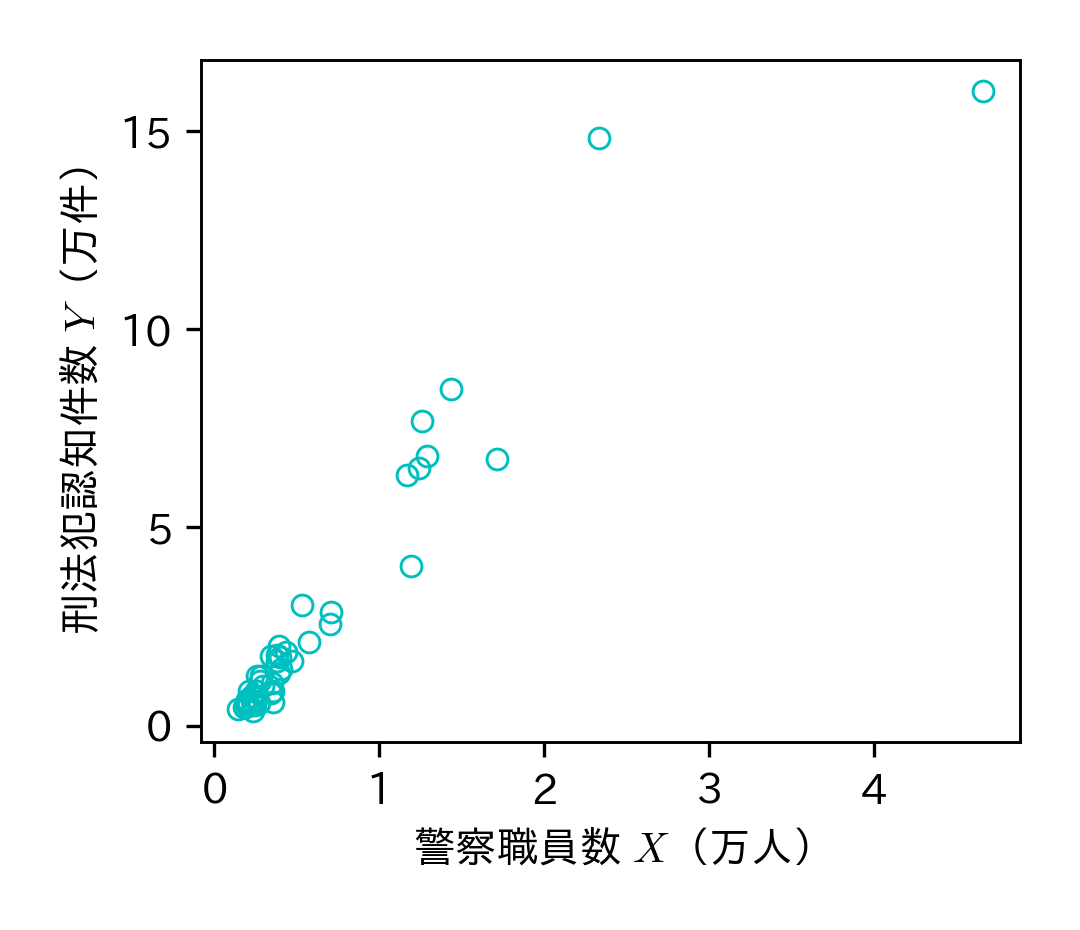
\includegraphics[width=6cm]{figure/police_crime.pdf}
	\caption{2015年の都道府県別警察職員数と刑法犯認知件数の散布図}
	\label{fig:police}
\end{figure}
%

\subsubsection*{STEP 4: Analysis}
%
まず,都道府県の人口を第3の変数と仮定し,警察職員数と刑法犯認知件数の関係が疑似相関であるか調べる.
%
\begin{itembox}[l]{実習}
%
\begin{itemize}
\item
刑法犯認知件数と警察職員数のそれぞれについて人口との散布図を描け.
\item
これらの散布図の相関係数を求め,それが何を意味するか考察せよ.
\end{itemize}
%
\end{itembox}
%

%%
%\begin{figure}[H]
%	\centering
%	\includegraphics[width=12cm]{figure/pop_crime_police.pdf}
%	\caption{A:人口と刑法犯罪認知件数の散布図.B:人口と警察職員数の散布図.}
%	\label{fig:police2}
%\end{figure}
%%

\vspace{0.5cm}
%
次に,疑似相関の有無についてさらに詳しく考察するため,人口の影響を取り除いた相関関係を調べる.
%
\begin{itembox}[l]{実習}
%
\begin{itemize}
\item
刑法犯認知件数と警察職員数の散布図について,人口が100万人未満,100万人以上200万人未満,200万人以上500万人未満で層別し,結果を考察せよ.
\item
人口1000人あたりの警察職員数と刑法犯罪認知件数に関する散布図を描いてその相関係数を求め,結果を考察せよ.
\item
人口の影響を除いた警察職員数と刑法犯認知件数の偏相関係数を求め,結果を考察せよ.
\end{itemize}
%
\end{itembox}
%

%%
%\begin{figure}[H]
%	\centering
%	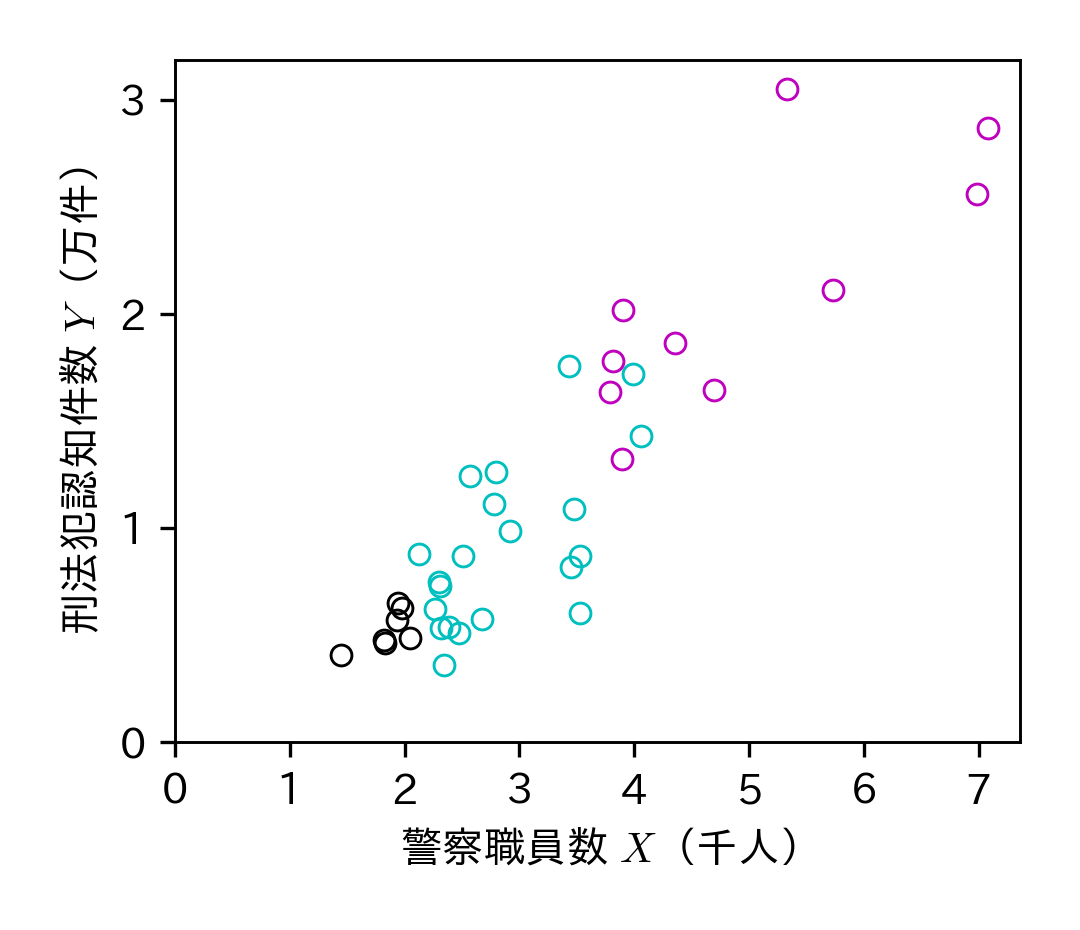
\includegraphics[width=6cm]{figure/police_crime2.pdf}
%	\caption{2015年の都道府県別警察職員数と刑法犯認知件数の層別散布図}
%	\label{fig:police3}
%\end{figure}
%%


%%
%\begin{figure}[H]
%	\centering
%	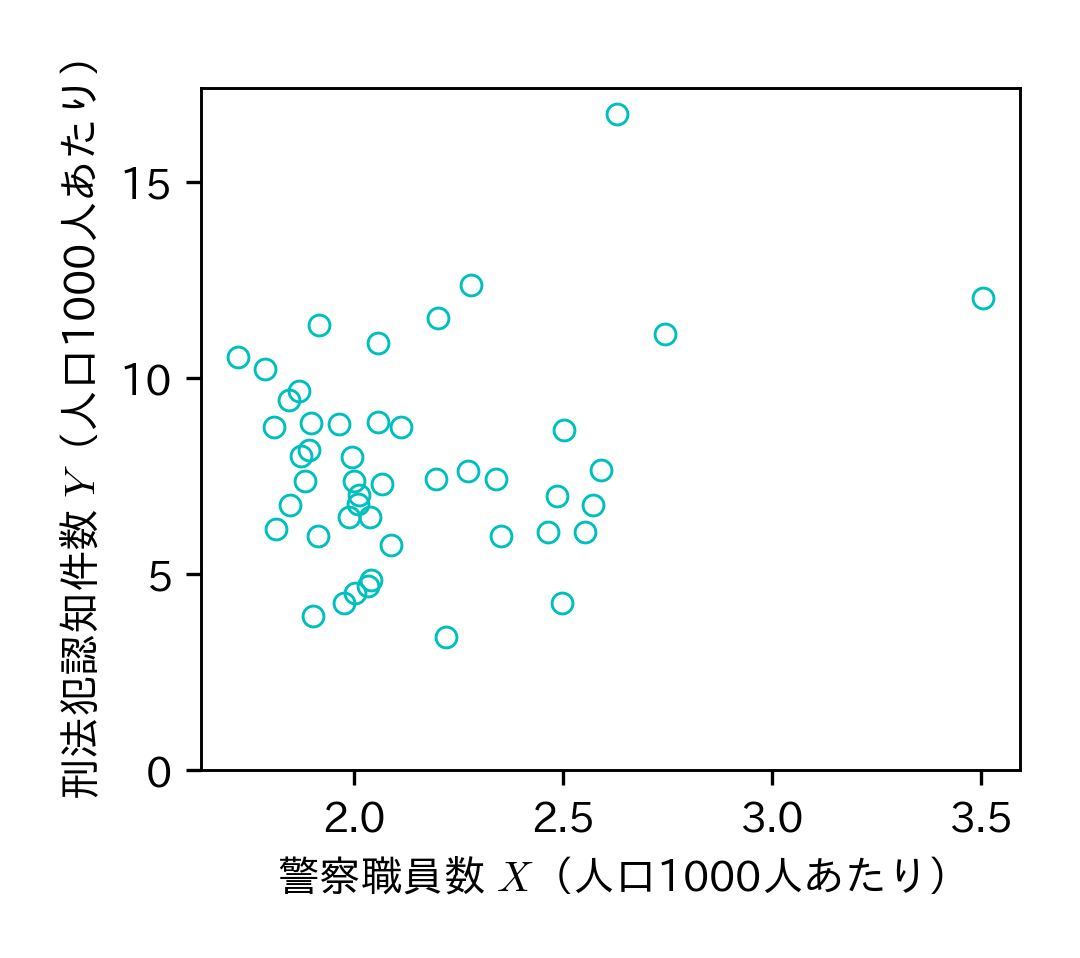
\includegraphics[width=6cm]{figure/police_crime3.pdf}
%	\caption{2015年の都道府県別警察職員数と刑法犯認知件数の散布図(人口1000人あたり)}
%	\label{fig:police4}
%\end{figure}
%%


\subsubsection*{STEP 5: Conclusion}
%%
%警察職員数と刑法犯認知件数は強い正の相関を示すが,これは人口を第3の変数とする疑似相関ということが分かった.
%%
%実際,第3の変数の影響を取り除くために,第3の変数による層別の方法,第3の単位あたりの量に変換する方法,偏相関係数を求める方法を適用すると,相関関係は見られなくなった.
%%

%
\begin{itembox}[l]{実習}
%
\begin{itemize}
\item
解析の結果から,警察職員数と刑法犯認知件数の間に因果関係があるかどうか考察せよ.
\end{itemize}
%
\end{itembox}
%

%\clearpage
%\subsection{実例:サービス経済化の状況とその背景を探る}
%
%\subsubsection*{STEP 1: Problem}
%%
%産業構造において,サービス業(第3次産業)の比率が高くなっていくことをサービス経済化と呼ぶ.
%%
%サービス経済化の実態は,どのような指標で捉えられるだろうか?また,その要因はなんだろうか?
%%
%
%\subsubsection*{STEP 2: Plan}
%%
%まず,サービス業に就業している人が実際に増加しているか,また,サービス業の生産活動が高まっているか確認する.
%%
%次いで,サービス経済化を解明するための仮設として受け入れられている\textbf{ペティ=クラークの法則}を統計データに基づいて検証する.
%%
%ペティ=クラークの法則とは,経済の発展につれて,国民経済に占める第1次産業(農林業,漁業など)の比重が次第に低下し,第2次産業(製造業,建設業など),次いで第3次産業(サービス業,金融,通信など)の比重が高まるという,産業構造の高度化を説明したものである\footnote{なお,最近では情報通信,医療,教育サービスなどを第4次産業と呼ぶことがある.}.
%%
%
%\subsubsection*{STEP 3: Data}
%%
%日本における産業別の就業者数は総務省「労働力調査」から取得した1953年以降のデータを利用する.
%%
%経済発展の度合いについては,1人当たり国民所得,1人当たりGDP,1人当たり所有資産などを用いることにする.
%%
%%産業別の経済活動については,内閣府「国民経済計算」のデータを利用する.
%%%
%%ただし,基準改定によって1990年以降とそれ以前で経済活動の範囲がやや変更になっていることに注意する.
%%
%
%\subsubsection*{STEP 4: Analysis}
%%
%図\ref{fig:service}に1人当たり実質GDPと第3次産業の就業者比率を併せて図示する.
%%
%第3次産業の就業者比率は1955年から2015年にかけて38.1\%から71.9\%に上昇しており,1人当たり実質GDPも同様の増加傾向を示している.
%%
%ペティ=クラークの法則を調べるため,図\ref{fig:service2}に1人当たり実質GDPと第3次産業就業率の散布図を示す.
%%
%この図より,確かに正の相関関係が明確に読み取れる.
%%
%実際,この散布図に対して相関係数を調べると,1に近い高い値が得られる.
%%
%
%%
%次に,世界各国のデータからもペティ=クラークの法則を検証してみる.
%%
%図\ref{fig:service3}は2014年の各国の1人当たり国民所得と第3次産業のGDP構成比の散布図を示している.
%%
%サウジアラビアを除けば,全体として2つの指標は高い相関を示していることが分かる.
%%
%
%%
%\begin{figure}[H]
%	\centering
%	\includegraphics[width=8cm]{figure/service.pdf}
%	\caption{1人当たり実質GDPと第3次産業就業率の推移}
%	\label{fig:service}
%\end{figure}
%%
%
%%
%\begin{figure}[H]
%	\centering
%	\includegraphics[width=8cm]{figure/service2.pdf}
%	\caption{1人当たり実質GDPと第3次産業就業率の散布図}
%	\label{fig:service2}
%\end{figure}
%%
%
%%
%\begin{figure}[H]
%	\centering
%	\includegraphics[width=8cm]{figure/service3.pdf}
%	\caption{1人当たり国民所得と第3次産業構成比の散布図}
%	\label{fig:service3}
%\end{figure}
%%
%
%\subsubsection*{STEP 5: Conclusion}
%%
%日本及び世界各国について,長期的な経済発展とともにサービス経済化が進展し,ペティ=クラークの法則が成り立っていることが確認できた.
%%


\clearpage
\section{散布図・相関分析による問題解決}

\subsection{回帰直線と最小二乗法}
%
2つの量的データ$ X $と$ Y $が与えられたとき,変数$ X $の値から$ Y $の値を予測するための数式のことを\textbf{回帰モデル}と呼ぶ.
%
また,$ X $を\textbf{説明変数(独立変数)},$ Y $を\textbf{目的変数(従属変数,被説明変数)}と呼ぶ.
%

%
例として,$ X $と$ Y $の散布図が図\ref{fig:lsm}のように与えられる場合を考える.
%
このとき,$ X $と$ Y $の間には直線関係が成り立ちそうである.
%
よって,回帰モデルとして,1次関数
%
\begin{align}
	\hat{y} &= ax + b
	\label{eq:regression_line}
\end{align}
%
を用いるのが妥当と考えられる.
%
この回帰モデルは\textbf{単回帰モデル}と呼ばれ,式\eqref{eq:regression_line}の直線のことを\textbf{回帰直線}と呼ぶ.
%
なお,$ a,\ b $は回帰直線の切片と傾きを表すパラメータであり,\textbf{回帰係数}と呼ばれる.
%

%
\begin{figure}[H]
	\centering
	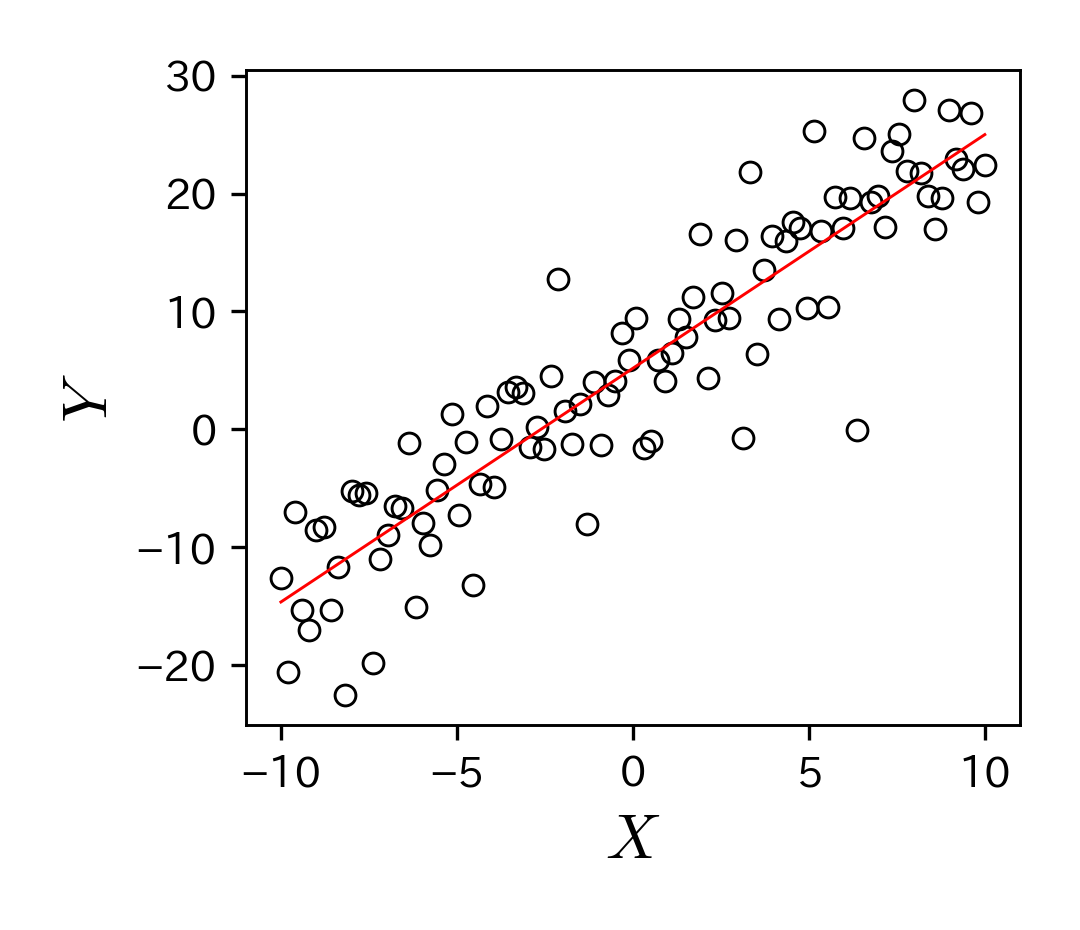
\includegraphics[width=7cm]{figure/lsm_ex.pdf}
	\caption{最小二乗法による回帰直線の例.}
	\label{fig:lsm}
\end{figure}
%


%
\subsubsection*{最小二乗法}
%
$ n $組のデータ$ (x_{i}, y_{i})\ (i=1, 2, \ldots, n) $が与えられたとき,式\eqref{eq:regression_line}を用いてデータから最適な回帰直線を求めることを\textbf{単回帰分析}と呼ぶ\footnote{説明変数が複数ある場合は重回帰分析と呼ぶ.}.
%
単回帰分析には様々な方法があるが,最も基本的な方法が\textbf{最小二乗法}である.
%
最小二乗法の発想は単純であり,予測値$ \hat{y}_{i}=ax_{i}+b $と実データ$ y_{i} $の差の二乗和(残差変動)
%
\begin{align*}
	E &= \sum_{i=1}^{n}(ax_{i}+b-y_{i})^{2}
\end{align*}
%
が最小となるような$ a,\ b $を回帰係数とするものである.
%
このための条件は,残差二乗和$ E $の$ a,\ b $による偏微分がゼロという式で与えられる:
%
\begin{align*}
	\frac{\partial E}{\partial a} &= 0, \hspace{0.5cm} \frac{\partial E}{\partial b} = 0 
\end{align*}
%
実際にこれらの条件を適用すると,$ a,\ b $は
%
\begin{align*}
	a &=\frac{\displaystyle\sum_{i=1}^{n} x_{i}y_{i} - \frac{1}{n} \sum_{i=1}^{n}x_{i}\sum_{i=1}^{n}y_{i}}{\displaystyle\sum_{i=1}^{n}x_{i}^{2} - \frac{1}{n} \left(\sum_{i=1}^{n}x_{i}\right)^{2}}=\frac{s_{XY}}{s^{2}_{X}}\\[10pt]
	b &= \bar{y} - a \bar{x} = \frac{1}{n} \sum_{i=1}^{n}(y_{i} - ax_{i})
\end{align*}
%
と表される.
%
なお,傾き$ a $は共分散$ s_{XY} $を$ X $の分散$ s^{2}_{X} $で割った形になっている(相関係数の式に似ているが違う).
%
よって,以下が成り立つ:
%
\begin{quotation}
共分散$ s_{XY} $が正,0,負 $ \Longleftrightarrow $ 最小二乗法による傾き$ a $が正,0,負
\end{quotation}
%
%特に,無相関(共分散$ s_{XY} $が0または相関係数が0)ならば最小二乗法による傾きが$ a=0 $となる.
%

\subsection{目的変数の変動と決定係数}
%
$ n $組のデータ$ (x_{i}, y_{i})\ (i=1, 2, \ldots, n) $に対して,次の3つの変動を考える.
%
\begin{enumerate}
%
\item{全変動(データ$ Y $のばらつき):$\displaystyle S_{y}^{2} = \sum_{i=1}^{n} (y_{i} - \bar{y})^{2}$}

\item{回帰変動(回帰モデルによる予測値のばらつき):$\displaystyle S_{\hat{y}}^{2} = \sum_{i=1}^{n} (\hat{y}_{i} - \bar{y})^{2}$}

\item{残差変動(実データと予測値のズレ):$\displaystyle S_{e}^{2} = \sum_{i=1}^{n} (y_{i} - \hat{y}_{i})^{2}$}
\end{enumerate}
%
単回帰分析の場合,以下の関係が成り立つ:
%
\begin{align*}
	S_{y}^{2} &= S_{\hat{y}}^{2} + S_{e}^{2}
\end{align*}
%

%
以上を踏まえ,回帰直線の当てはまりの良さを示す\textbf{決定係数}を
%
\begin{align}
	R^{2} &= \frac{S_{\hat{y}}^{2}}{S_{y}^{2}} = 1 - \frac{S_{e}^{2}}{S_{y}^{2}}
	\label{eq:R2}
\end{align}
%
と定義する\footnote{他の定義もあるので注意.}.
%
これは,全変動と回帰変動の比として定義されるので,実データの変動のうち,どの程度が回帰モデルで説明できるのかを表す量である.
%
特に,式\eqref{eq:R2}より定義域は$ 0 \leq R^{2} \leq 1 $であり,残差変動が0に近づく(データへの当てはまりが良い)と$ R^{2} $は1に近づく.
%
一方,残差変動が大きくなる(データへの当てはまりが悪い)と$ R^{2} $は0に近づく.
%
なお,予測値$ \hat{y} $が最小二乗法によって決められた場合,決定係数は相関係数の二乗に等しい.
%

\subsection{実例:都市の平均気温と緯度の関係}

\subsubsection*{STEP 1: Problem}
%
地球上では,赤道付近は暑く,極地に近づくほど寒くなる.
%
世界の様々な地域の年間平均気温はどのように決まっているのだろうか?
%

\subsubsection*{STEP 2: Plan}
%
世界の各地域で年間平均気温は異なっている.
%
各地域での年間平均気温に影響を与える要因は,図\ref{fig:fish_bone}のような図にまとめることができる.
%
これを\textbf{特性要因図}と呼ぶ.
%
ここには,各地域の地球上での位置,都市の自然環境,人間活動が要因として挙げられている.
%
以下では,各都市の地球上での位置に関するデータを収集し,年間平均気温との関係を探る.
%

%
\begin{figure}[H]
	\centering
	\includegraphics[width=8cm]{figure/fish_bone.pdf}
	\caption{特性要因図.都市の年間平均気温に影響を与える要因.}
	\label{fig:fish_bone}
\end{figure}
%

\subsubsection*{STEP 3: Data}
%
世界各都市の年間平均気温は理科年表や気象庁のHPで調べることができる.
%
表\ref{tb:temp}は理科年表から得られた各都市の年間平均気温,緯度,標高のデータである.
%

\begin{table}[H]
    \centering
    \caption{世界の25都市の年間平均気温,緯度,標高}
	\label{tb:temp}
	\scalebox{0.7}{
    \begin{tabular}{|c|c|c|c|c|c|c|c|c|}
    \hline
        地名 & 平均気温(℃) & 緯度(度) & 標高($ m $) & & 地名 & 平均気温(℃) & 緯度(度) & 標高($ m $) \\ \hline\hline
        昭和基地 & -10.5 & -69.00 & 18 & & ドーハ & 27.0 & 25.15 & 11 \\ \hline
        メルボルン & 14.5 & -37.39 & 132 & & カイロ & 21.7 & 30.06 & 116 \\ \hline
        ブエノスアイレス & 17.8 & -34.35 & 25 & & ケープタウン & 16.8 & 33.58 & 46 \\ \hline
        ブリスベン & 20.3 & -27.23 & 4 & & 東京 & 15.4 & 35.42 & 25 \\ \hline
        リオデジャネイロ & 23.9 & -22.55 & 5 & & サンフランシスコ & 14.5 & 37.37 & 6 \\ \hline
        リマ & 19.3 & -12.01 & 12 & & 北京 & 12.9 & 39.56 & 55 \\ \hline
        ジャカルタ & 28.0 & -6.11 & 8 & & サラエボ & 10.4 & 43.52 & 630 \\ \hline
        シンガポール & 27.6 & 1.22 & 5 & & リオン & 11.9 & 45.43 & 197 \\ \hline
        ボゴダ & 13.4 & 4.42 & 2547 & & チュリッヒ & 9.4 & 47.22 & 555 \\ \hline
        コロンボ & 27.7 & 6.54 & 7 & & プラハ & 8.4 & 50.06 & 380 \\ \hline
        アジスアベベ & 16.6 & 9.02 & 2354 & & ダブリン & 9.8 & 53.26 & 68 \\ \hline
        チェンマイ & 29.0 & 13.00 & 13 & & レイキャビク & 4.7 & 64.08 & 54 \\ \hline
        メキシコ & 16.7 & 19.24 & 2309 & &   &  &  &  \\ \hline
    \end{tabular}
    }
\end{table}

\subsubsection*{STEP 4: Analysis}

\subsubsection*{散布図}
%
まず,平均気温と他の量との相関関係を視覚的に確認するために散布図を調べることにする.
%
図\ref{fig:lat_alt_temp}は緯度と平均気温,標高と平均気温の散布図である.
%

%
\begin{figure}[H]
	\centering
	\includegraphics[width=12cm]{figure/lat_alt_temp.pdf}
	\caption{緯度・標高と平均気温の関係}
	\label{fig:lat_alt_temp}
\end{figure}
%

%
図\ref{fig:lat_alt_temp}を見ると,平均気温は緯度に対して上に凸の2次関数のような関係となり,かつ赤道(0度)に対して左右対称になっていることが分かる.
%
一方,標高と平均気温については特定の関数関係はない.
%
このように,散布図がそもそも直線関係となっていない場合には,相関係数を求めるのは不適切である.
%
%2つの量の間の相関関係を調べる際には,まず散布図を描くことが鉄則である.
%

\subsubsection*{緯度と平均気温の関数関係}
%
緯度と平均気温の関数関係を特定すれば,散布図が直線関係を示すような適切な変数変換を導ける.
%
そこで,緯度の値別に複数のグループに分け,グループ内で平均気温,平均緯度などを求めて関係を調べることにする.
%
具体的に,ここでは25都市を緯度の絶対値の昇順に5都市ずつのグループに分ける:
%
\begin{description}
\item{群1:}
シンガポール,ボコタ,ジャカルタ,コロンボ,アジスアベバ
\item{群2:}
リマ,チェンマイ,メキシコ,リオデジャネイロ,ドーハ
\item{群3:}
ブリスベン,カイロ,ケープタウン,ブエノスアイレス,東京
\item{群4:}
サンフランシスコ,メルボルン,北京,サラエボ,リオン
\item{群5:}
チューリッヒ,プラハ,ダブリン,レイキャビク,昭和基地
\end{description}
%

%
\begin{itembox}[l]{実習}
%
\begin{itemize}
\item
各群に対し,絶対緯度の平均,平均気温の平均,平均気温の標準偏差を求めよ
\item
平均絶対緯度を横軸,平均気温の平均を縦軸に取った図をエラーバー付きで描け
\end{itemize}
%
\end{itembox}
%

\vspace{0.5cm}
%
実際に平均絶対緯度を横軸,平均気温の平均を縦軸に取った図を描くと,絶対緯度と平均気温の関係は2次関数的な変化となっていることが分かる.

%
\begin{itembox}[l]{実習}
%
\begin{itemize}
\item
横軸に絶対緯度の2乗,縦軸に平均気温を取った散布図を描け
\item
この散布図に対して,相関係数を求めよ
\item
この散布図に対して,最小二乗法で回帰直線を求めよ
\end{itemize}
%
\end{itembox}
%

%%
%\begin{figure}[H]
%	\centering
%	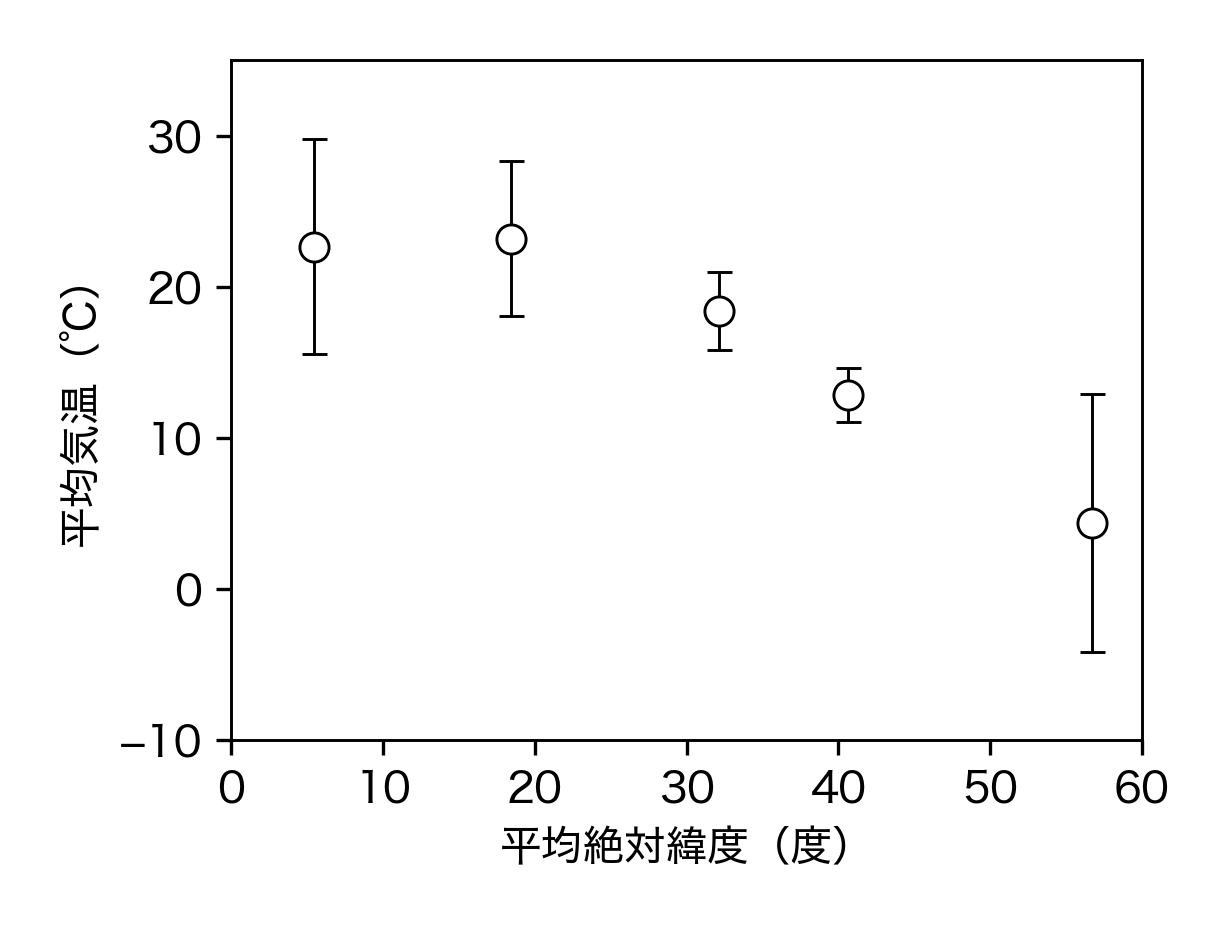
\includegraphics[width=8cm]{figure/ave_latitude_temp.pdf}
%	\caption{平均気温と平均絶対緯度の関係}
%	\label{fig:ave_latitude_temp}
%\end{figure}
%%
%
%%
%\begin{figure}[H]
%	\centering
%	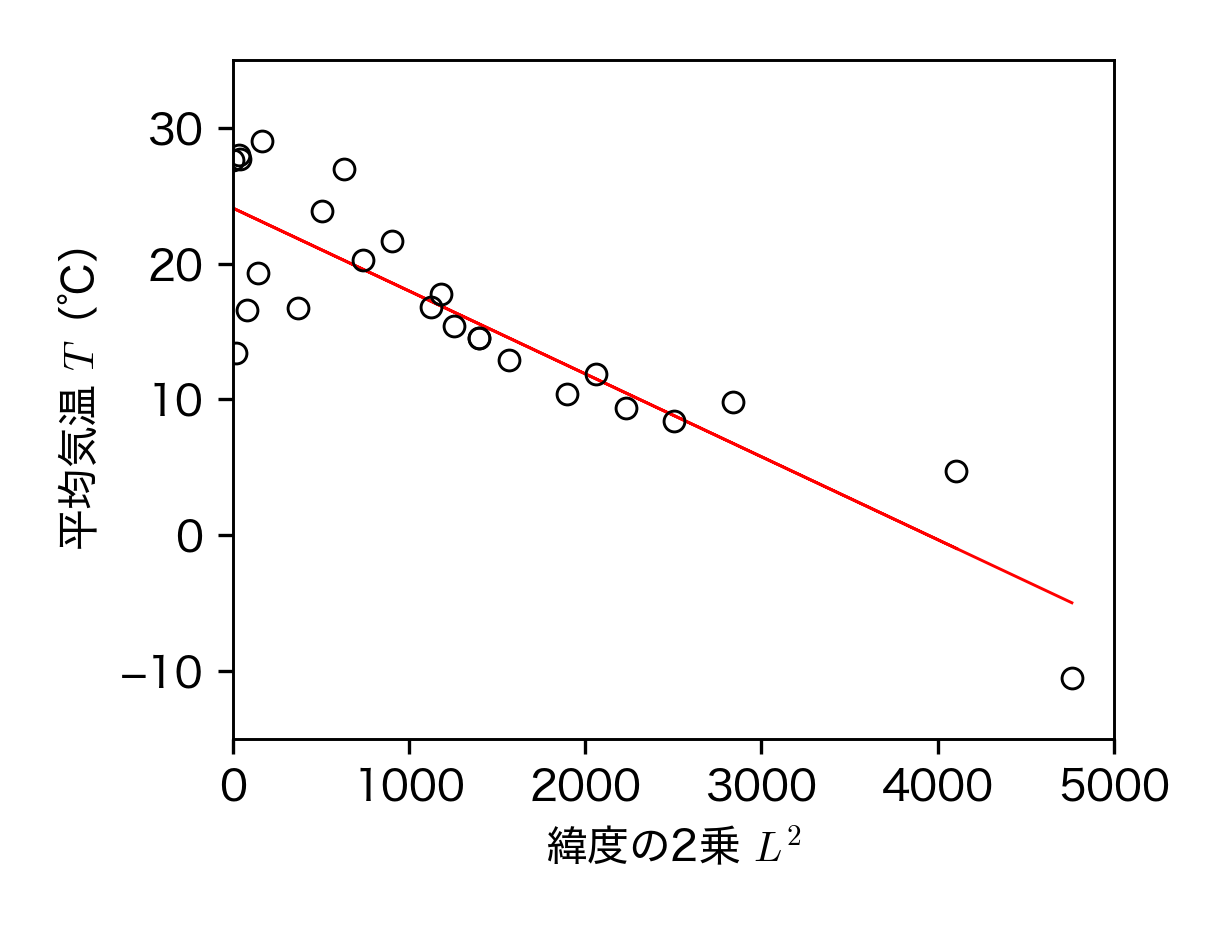
\includegraphics[width=8cm]{figure/lat2_temp.pdf}
%	\caption{緯度の2乗と平均気温の散布図}
%	\label{fig:scatter_sqlatitude_temp}
%\end{figure}
%%

\subsubsection*{Step 5: Conclusion}
%
各都市の年間平均気温と緯度の関係を散布図によって調べた結果,緯度の2乗に対して直線関係があることが分かった.
%
一方,年間平均気温が緯度の2次関数になるということは,緯度が高くなれば気温もいくらでも大きくなることを意味し,やや奇妙である.

%
\vspace{0.5cm}
\begin{itembox}[l]{実習}
%
\begin{itemize}
\item
緯度$ \theta $における太陽エネルギーは$ \cos\theta $に比例することが知られている.
これより,年間平均気温と緯度を結びつける,より適切な関数を求めよ.
\item
テイラー展開の観点から,2次関数の妥当性を議論せよ.
\end{itemize}
%
\end{itembox}
%

%%
%
%%
%また,物理的な考察により,コサイン関数がより適切であることが分かった.
%%

\subsubsection*{Step 6: Problem 2}
%
緯度の2乗と平均気温の散布図を見ると,直線関係から少し外れる都市がいくつかあることが分かる.
%
これらの都市は,外れ値の大きい順にボコダ,メキシコ,アジスアベバ,である.
%
では,これらの都市はなぜ直線関係から外れるのだろうか?

\subsubsection*{Step 7: Plan \& Data 2}
%
直線から外れている都市について,表\ref{tb:temp}を見てみると,ある共通点が浮かび上がる.
%
それは,標高が高いことである(いずれも標高2000m以上).
%
一般的に,標高が高くなるほど都市の気温は低くなる.
%
よって,平均気温と緯度の関係を見るためには,標高の影響を調整する必要がある.
%
一般に,標高が100m高くなると,気温は0.6℃低くなると言われている.
%
これより,平均気温($ T $)に対して標高($ z $)の影響を調整した気温(高度調整済み平均気温)は$ T_{0}=T+0.006z $と表される.
%

\subsubsection*{Step 8: Analysis 2}

%
\begin{itembox}[l]{実習}
%
\begin{itemize}
\item
緯度の2乗と高度調整済み平均気温の散布図を描け
\item
この散布図から相関係数を求めよ
\item
この散布図に対して回帰直線を引き,直線の式を求めよ
\end{itemize}
%
\end{itembox}
%

\subsubsection*{Step 9: Conclusion 2}
%
年間平均気温と緯度の2乗の関係において発生する外れ値は,標高の影響によるものであることが分かった.
%
そこで,標高の影響を調整することで,年間平均気温,緯度,標高に対する適切な関数を推定することができた.
%


\chapter{確率と確率変数}

\section{確率の概念}

\subsection{標本空間と事象}
%
サイコロを振ったりコインを投げるなど,同じ条件で繰り返すことができる操作を\textbf{試行}と呼び,試行の結果起こりうる事柄を\textbf{事象}と呼ぶ.
%
また,ある試行によって起こりうる個々の結果を\textbf{標本点}$ \omega $,その全体の集合を\textbf{標本空間}$ \Omega $と表す.
%
%例えば,サイコロを1回投げた場合の標本空間は$ \Omega=\{1,2,3,4,5,6\} $であり,$ 1 $や$ 2 $などが標本点である.
%%
%もし,サイコロを2回投げる場合には標本空間は36個の標本点から成る:$ \Omega=\{(1,1), (1,2),\ldots, (6,6)\} $.
%

%
事象は集合を使って整理することができ,より正確には標本空間の\textbf{部分集合}によって定義される.
%
ここで,$ A $が$ B $の部分集合であるとは,$ A $のすべての構成要素が$ B $の構成要素である場合をいい,$ A \subset B $と表す.
%
標本点$ \omega_{1}, \cdots, \omega_{n} $から成る事象$ A $は$ A = \{\omega_{1}, \cdots, \omega_{n}\} $のように表す.
%
なお,標本空間$ \Omega $自体を\textbf{全事象},標本点を1つも含まない集合を\textbf{空事象}$ \phi $と呼び,これらも事象と見なす.
%
一般に,標本空間が$ r $個の標本点から成る場合,事象(部分集合)は$ 2^{r} $個存在する.
%

%
例えば,コインを1回投げる場合,「表」と「裏」が標本点であり,標本空間は
%
\begin{align*}
	\Omega &= \{表, 裏\}
\end{align*}
%
となる.
%
また,標本点の数が$ r=2 $なので,事象は以下のように$ 2^{2}=4 $個ある:
%
\begin{align*}
	\{表, 裏\}, \{表\}, \{裏\}, \phi
\end{align*}
%
ここで,$ \{表, 裏\} $が全事象に対応し,コインを1回投げて表または裏が出るという事象を表わす.
%
サイコロを2個同時に投げる場合の標本空間は36個の標本点から成る:$ \Omega=\{(1,1), (1,2),\ldots, (6,6)\} $.
%
特に,目の合計が7となる事象は
%
\begin{align*}
	A = \{(1,6), (2,5), (3,4), (4,3), (5,2), (6,1)\}
\end{align*}
%
である.
%

%
事象のうち,ただ1つの標本点から成りそれ以上分解できないものを\textbf{根元事象}と呼び,一方で複数の標本点を含み2つ以上の根元事象に分解可能なものは\textbf{複合事象(結合事象)}と呼ぶ.
%
例えば,サイコロを1回投げた場合,$ \{1\}, \{2\} $は根元事象であるが,$ \{1, 3, 5\} $(偶数の目が出る)は複合事象である.
%

%
以上のように,標本点が有限個の点から成る場合もあるが,長さ,重さ,温度など,ある区間内のすべての点を取りうる場合には標本空間は無限個の点から成る無限集合である.
%
例えば,電球の寿命は確率的と考えられるが,標本空間は
%
\begin{align*}
	\Omega &= (0, \infty)
\end{align*}
%
である.
%
このとき,1000時間目に電球がまだ正常であるという事象は$ A = (1000, \infty) $である.
%

\subsubsection*{事象の演算}
%
事象を表すのに便利な方法として,\textbf{ベン図}がある.
%
これは,標本点の数に関わらず標本空間を長方形で表し,各事象を長方形の内部に円で示す方法である.
%
2つの事象$ A,\ B $の関係は以下の3つに分類できる(図\ref{fig:venn}):
%
(a) $ A $は$ B $の部分集合である,(b) $ A $は$ B $の部分集合でないが,$ A $と$ B $は共通部分を持つ,(c) $ A $と$ B $は共通部分を持たない.
%
この中で,(c)の場合,一方が起これば他方は起こらないので,$ A $と$ B $は\textbf{排反事象}または\textbf{互いに排反}であるという.
%

%
\begin{figure}[H]
	\centering
	\includegraphics[width=10cm]{figure/venn.pdf}
	\caption{ベン図による2つの事象の関係の図示.}
	\label{fig:venn}
\end{figure}
%

%
$ A $と$ B $の2つの事象のうち少なくとも1つが起こる($ A $または$ B $が起こる)という事象を,$ A $と$ B $の\textbf{和事象}と呼び,$ A \cup B $で表す($ \cup $の記号は``または''や``カップ''などと読む).
%
例えば,サイコロを1回投げる場合,$ A $を奇数の目が出る事象,$ B $を3以下の目が出る事象とすると,$ A\cup B = \{1,3,5\} \cup \{1,2,3\} = \{1,2,3,5\} $である.
%

%
$ A $と$ B $が同時に起こる($ A $かつ$ B $が起こる)という事象は,\textbf{積事象}と呼ばれ,$ A\cap B $と表される($ \cap $の記号は``かつ''や``キャップ'',``共通部分''などと読む).
%
例えば,サイコロを1回投げる場合,$ A $を奇数の目が出るという事象,$ B $を3以下の目が出るという事象とすると,$ A\cap B = \{1,3,5\} \cap \{1,2,3\} = \{1,3\} $である.
%
なお,$ A $と$ B $の共通部分がない場合には$ A \cap B = \phi $である.
%

%
3つの事象$ A,\ B,\ C $に対して,以下の分配法則が成り立つ:
%
\begin{align*}
	(A\cup B) \cap C &= (A\cap C) \cup (B\cap C) \\
	(A\cap B) \cup C &= (A\cup C) \cap (B\cup C)
\end{align*}
%

%
事象$ A $が起こらないという事象は$ A $の\textbf{補事象(余事象)}と呼び,$ A^{c} $または$ \bar{A} $と表す.
%
また,事象$ A, B $に対し,以下の\textbf{ド・モルガンの法則}が成り立つ:
%
\begin{align*}
	(A\cup B)^{c} &= A^{c} \cap B^{c}, \hspace{0.5cm} (A\cap B)^{c} = A^{c} \cup B^{c}
\end{align*}
%
例えば,$ A $をスペードが出る,$ B $を絵札が出るという事象とすると,「スペードまたは絵札が出る」($ A \cup B $)の補事象は「スペードが出ず,かつ絵札も出ない」($ A^{c} \cap B^{c} $)である.
%

\subsection{確率の定義}

\subsubsection*{ラプラスの定義}
%
ある試行について,根元事象が$ N $個あり(つまり,標本空間の大きさが$ N $),それらが同程度に確からしく起こるとする.
%
このとき,事象$ A $に対応する根元事象が$ R $個あれば,事象$ A $の確率は
%
\begin{align*}
	P(A) &= R/N
\end{align*}
%
と定義される.
%
例えば,サイコロを1回投げて奇数の目が出るという事象を$ A $とすると,その確率は$ N=6 $,$ R=3 $なので$ P(A)=3/6=1/2 $である.
%

%
以上の定義の利点は,確率が標本点の個数,すなわち起こり方の場合の数の数え上げに帰することであり,順列,組み合わせの諸定理が使えることである.
%
一方,問題点は,各標本点が同様に確からしく起こると仮定していることである.
%
例えば,サイコロの場合は各目が同程度の確かさで出現すると仮定しているが,これが正しい保証はない.
%

\subsubsection*{頻度による定義}
%
ラプラスの定義はサイコロやコインなどについては有益であるが,各標本点が同程度に確からしく起こると考えられない場合には適用できない.
%
そこで,より実際的な定義として,以下のような頻度による定義(頻度説)がある.
%
ある試行を$ n $回繰り返し,事象$ A $が生じた回数(頻度または度数)$ n_{A} $を数える実験を行う.
%
いま,$ n\to \infty $としたとき,その相対頻度(相対度数)が
%
\begin{align*}
	\lim_{n\to \infty} \frac{n_{A}}{n} = \alpha
\end{align*}
%
となるならば,$ P(A)=\alpha $と定義する.
%

%
一般に,相対頻度$ n_{A}/n $は真の確率$ P(A) $と一致せず,試行回数$ n $が同じでも各回ごとに異なる値が観測される.
%
しかし,いずれの場合も$ n $が大きくなるに従い,相対頻度は真の値とほとんど等しくなる様子が観察され,これを確率と見なすのが頻度説である.
%
このように,頻度説は無限の試行によって初めて正当化されるので,あくまでも理論上の仮定の上に成り立っている.
%

\subsubsection*{公理主義的な定義}
%
確率と事象の関係を規定し,確率を数学的に構成するためには,公理\footnote{数学的な体系を構築する上で,無条件で正しいとする前提,仮定}を設けてそれに基づいて体系的に議論する必要がある.
%
この考えに基づくのが以下に示す確率の公理主義的定義である.
%

%
\begin{quotation}
標本空間$ \Omega $の事象$ A $に対して次の3つの条件を満たす実数$ P(A) $が存在するとき,$ P(A) $を事象$ A $が起こる確率という:
%
\begin{enumerate}
\item
$  0 \leq P(A) \leq 1 $
\item
$ P(\Omega) = 1 $
\item
互いに排反な事象$ A_{1},\ A_{2},\ \ldots $に対し,
%
\begin{align*}
	P(A_{1} \cup A_{2} \cup \cdots) &= P(A_{1}) + P(A_{2}) + \cdots
\end{align*}
%
\end{enumerate}
%
\end{quotation}
%

%
これらの公理のうち,3つ目は経験的確率の性質を一般的に書いたものである.
%
例えば,サイコロを振って偶数の目が出るという事象$ A_{1} $の確率は$ P(A_{1})=3/6 $,3の目が出るという事象$ A_{2} $の確率は$ P(A_{2})=1/6 $であり,これらは排反事象である.
%
このとき,偶数の目または3の目が出るという事象の確率は$ P(A_{1} \cup A_{2})=3/6 + 1/6 $によって計算できる.
%

\subsection{確率の性質}
%
以下では,確率の公理主義的な定義を前提とする.

\subsubsection*{加法定理}
%
事象$ A $と$ B $が互いに排反(共通部分を持たない)であるとき,公理より
%
\begin{align*}
	P(A \cup B) &= P(A) + P(B)
\end{align*}
%
が成り立つ.
%

%
一方,事象$ A $と$ B $が排反ではなく,共通部分を持つ場合には
%
\begin{align*}
	P(A \cup B) &= P(A\cap B^{c}) + P(A^{c}\cap B) + P(A\cap B)
\end{align*}
%
が成り立つ.
%
また,$ A = (A\cap B^{c}) \cup (A\cap B) $であり,$ A\cap B^{c} $と$ A\cap B $は排反事象なので,
%
\begin{align*}
	P(A) &= P(A\cap B^{c}) + P(A\cap B)
\end{align*}
%
同様にして,
%
\begin{align*}
	P(B) &= P(A\cap B) + P(A^{c}\cap B)
\end{align*}
%
である.
%
以上より,
%
\begin{align*}
	P(A\cup B) &=  P(A) + P(B) - P(A \cap B)
\end{align*}
%
が成り立つ.
%
これを\textbf{確率の加法定理}と呼ぶ.
%

%
例えば,ジョーカーを含むトランプ53枚から1枚取り出す場合を考える.
%
カードがスペードであるという事象を$ A $とすると,$ P(A)=13/53 $である.
%
また,カードが絵札であるという事象を$ B $とすると,$ P(B)=12/53 $である.
%
さらに,スペードの絵札である確率は$ P(A\cap B)=3/53 $である.
%
よって,加法定理を用いると,カードがスペードかまたは絵札である確率は
%
\begin{align*}
	P(A\cup B) &= 13/53+12/53-3/53=22/53
\end{align*}
%
となる.
%


\subsubsection*{条件付き確率}
%
2つの事象$ A,\ B $があるとき,事象$ A $が起こったという条件の下で$ B $が起こるという事象を$ B|A $と表す.
%
また,その確率$ P(B|A) $を条件$ A $の下での$ B $の\textbf{条件付き確率}といい,
%
\begin{align*}
	P(B|A) &= \frac{P(A\cap B)}{P(A)}
\end{align*}
%
と定義する(ただし,$ P(A)\neq 0 $).
%

%
例として,トランプから1枚のカードを取り出す場合を考える.
%
カードがスペードであるという事象を$ A $,絵札であるという事象を$ B $とする.
%
このとき,$ B|A $はカードがスペードであると分かった場合にそれが絵札であるという事象を意味する.
%
スペードのカードは13枚あり,そのうち絵札は3枚なので,$ P(B|A)=3/13 $である.
%
一方,スペードである確率は$ P(A)=13/53 $,スペードでありかつ絵札である確率は$ P(A\cap B)=3/53 $であるから,条件付き確率の定義より$ P(B|A)=\frac{3/53}{13/53}=3/13 $となり定義を満たすことが分かる.
%

\vspace{0.5cm}
%
なお,条件$ B $の下での$ A $の条件付き確率$ P(A|B) $も同様に定義でき,
%
\begin{align*}
	P(A|B) &= \frac{P(A\cap B)}{P(B)}
\end{align*}
%
が成り立つ(ただし,$ P(B)\neq 0 $).
%
よって,これらの式を変形すれば以下が成り立つ:
%
\begin{align*}
	P(A\cap B) &= P(B|A)P(A) = P(A|B)P(B)
\end{align*}
%
これを\textbf{確率の乗法定理}と呼ぶ.
%

\subsubsection*{独立性}
%
条件付き確率$ P(A|B) $は$ B $が起こったという条件の下で$ A $が起こる確率であるが,$ B $が$ A $に何の影響も及ぼさない場合もある.
%
このようなときは
%
\begin{align*}
	P(A|B) &= P(A)
\end{align*}
%
が成り立ち,乗法定理は
%
\begin{align*}
	P(A\cap B) &= P(A)P(B)
\end{align*}
%
となる.
%
以上2つの式が成り立つとき,事象$ A $と$ B $は\textbf{統計的に独立}であるという.
%
なお,これは$ n $個の事象$ A_{1},\ A_{2},\ \cdots, A_{n} $についても成り立ち,
%
\begin{align*}
	P(A_{1}\cap A_{2}\cap \cdots \cap A_{n}) &= P(A_{1})P(A_{2})\cdots P(A_{n})
\end{align*}
%
のときに事象$ A_{1},\ A_{2},\ \cdots, A_{n} $は独立である.
%

%\vspace{0.5cm}
%\begin{itembox}[l]{実習}
%%
%ゆがんだコインを投げて表が出る確率を$ P(H)=p $とする.
%%
%%
%\begin{itemize}
%\item
%このコインを投げ続けて5回目に初めて表が出る確率はいくらか?
%\item
%このコインを5回投げて,表が3回出る確率はいくらか?
%\end{itemize}
%%
%\end{itembox}

%\vspace{0.5cm}
%\begin{itembox}[l]{実習}
%%
%青いカード$ b $,白いカード$ w $枚を合計$ b+w $枚入れた箱からよくかき混ぜてカードを抜き出す.
%%
%結果について,1枚目が青ならば$ B_{1} $などと表記する.
%%
%\begin{description}
%\item{(a)}元に戻さずに抜き出すとき,条件付き確率$ P(W_{2}|B_{1}) $を求めよ.
%\item{(b)}元に戻さずに抜き出すとき,確率$ P(B_{1}\cap W_{2}) $を求めよ.
%\item{(c)}元に戻さずに抜き出すとき,確率$ P(B_{1}\cap W_{2}\cap W_{3}) $を求めよ.
%\item{(d)}元に戻さずに抜き出すとき,確率$ P(W_{2}) $を求めよ.
%\item{(e)}毎回元に戻しながら抜き出すとき,確率$ P(B_{1}\cap W_{2}\cap W_{3}) $を求めよ.
%\end{description}
%%
%\end{itembox}
%
%\vspace{0.5cm}
%\begin{itembox}[l]{実習}
%%
%箱の中に数字を書いたカードが6枚あり,その数字は3枚が「1」,2枚が「2」,1枚が「4」である.
%%
%よくかき混ぜて毎回元に戻しながらカードを抜き出すとき,以下の確率はいくらか?
%%
%\begin{description}
%\item{(a)} 3回の実験でいずれも「1」が出る.
%\item{(b)} 3回の実験で「1」,「1」,「2」の順に出る.
%\item{(c)} 3回の実験で「1」,「2」,「1」の順に出る.
%\item{(d)} 3回の実験で「1」が2回,「2」が1回出る.
%\item{(e)} 5回目に初めて「4」が出る.
%\item{(f)} 「1または2」が出る前に「4」が出る.
%\end{description}
%%
%\end{itembox}
%
%\vspace{0.5cm}
%\begin{itembox}[l]{実習}
%%
%箱の中に数字を書いたカードが6枚あり,その数字は3枚が「1」,2枚が「2」,1枚が「4」である.
%%
%よくかき混ぜて毎回元に戻さずにカードを取り出すとき,以下の確率はいくらか?
%%
%\begin{description}
%\item{(a)} 1枚目に「1」が出たという条件の下で,2枚目に「4」が出る.
%\item{(b)} 3回の実験で,「1」,「1」,「2」の順に出る.
%\item{(c)} 3回の実験で,順番に関わらず「1」が2枚,「2」が1枚出る.
%\item{(d)} 1枚目の結果に関わらず,2枚目に「2」が出る.
%\item{(e)} 1枚目を伏せた状態で2枚目に「2」が出たとき,1枚目を見たら「2」となる.(\textbf{主観確率})
%\end{description}
%%
%\end{itembox}

%\vspace{0.5cm}
%\begin{itembox}[l]{実習}
%%
%A,B,Cの3人があるゲームをするとき,それぞれが勝つ確率を$ P(A)=a $,$ P(B)=b $,$ P(C)=c $とする($ a+b+c=1 $).
%%
%このとき,Bが初めて勝つ前にAが初めて勝つ確率はいくらか?
%%
%\end{itembox}

\subsection{ベイズの公式}
%
事象$ B_{1}, B_{2},\ \cdots, B_{n} $は互いに排反で,かつ$ B_{1}\cup B_{2} \cup \cdots \cup B_{n} = \Omega $が成り立つとする.
%
このとき,ある事象$ A $に対し,乗法公式より
%
\begin{align*}
	P(A|B_{i})P(B_{i}) &= P(B_{i}|A)P(A)
\end{align*}
%
両辺の$ i $について和をとれば,
%
\begin{align*}
	\sum_{i} P(A|B_{i})P(B_{i}) &= \sum_{i} P(B_{i}|A)P(A) \\
	                            &= P(A)
\end{align*}
%
となる(\textbf{全確率の定理}).
%
これより,
%
\begin{align*}
	P(B_{i}|A) &= \frac{P(A|B_{i})P(B_{i})}{P(A)} = \frac{P(A|B_{i})P(B_{i})}{\sum_{i} P(A|B_{i})P(B_{i})}
\end{align*}
%
が成り立つ.これを\textbf{ベイズの公式}と呼ぶ.
%

%
いま,$ B_{i} $を原因,$ A $を与えられた結果と見なすと,原因$ B_{i} $が起こる確率$ P(B_{i}) $と条件付き確率$ P(A|B_{i}) $が分かれば,結果$ A $から原因の確率$ P(B_{i}|A) $を計算できることを意味する.
%
ここで,$ P(B_{i}) $は\textbf{事前確率},$ P(B_{i}|A) $は\textbf{事後確率},$ P(A|B_{i}) $は\textbf{尤度}と呼ばれる.


\vspace{0.5cm}
\textbf{例1)}ある製品を作る機械$ B_{1} $,$ B_{2} $,$ B_{3} $がある.
%
この製品を作るときに,各機械が使われる割合(確率)はそれぞれ$ P(B_{1})=0.5 $,$ P(B_{2})=0.3 $,$ P(B_{3})=0.2 $である.
%
いま,出来上がった製品が不良品であるという事象を$ A $とする.
%
各機械が不良品を出す割合がそれぞれ$ 1\%,1.5\%,2\% $であるとすれば
%
\begin{align*}
	&P(A|B_{1}) = 0.01, \hspace{0.5cm} P(A|B_{2}) = 0.015, \hspace{0.5cm} P(A|B_{3}) = 0.02\\
	&P(A) = P(A|B_{1})P(B_{1}) + P(A|B_{2})P(B_{2}) + P(A|B_{3})P(B_{3}) = 0.0135
\end{align*}
%
となる.
%
このとき,出来上がった製品が不良品であったとき,使われた機械が$ B_{i} $であった確率はベイズの公式よりそれぞれ
%
\begin{align*}
	P(B_{1}|A) &= \frac{P(A|B_{1})P(B_{1})}{P(A)} = 0.3704 \\
	P(B_{2}|A) &= \frac{P(A|B_{2})P(B_{2})}{P(A)} = 0.3333 \\
	P(B_{3}|A) &= \frac{P(A|B_{3})P(B_{3})}{P(A)} = 0.2963 
\end{align*}
%
と求まる.すなわち,この場合は機械$ B_{1} $で作られた可能性が最も高い(機械$ B_{1} $の性能は最も高いことに注意).

\vspace{0.5cm}
\textbf{例2)}新型コロナウイルスのPCR検査によって陽性になるという事象を$ A $とする.
%
また,新型コロナウイルスに感染するという事象を$ B $とする.
%
いま,市中感染率はP(B)=0.1\%で,PCR検査の偽陰性率は30\%,偽陽性率は1\%と仮定すれば,尤度と全確率は
%
\begin{align*}
	&P(A|B) = 0.7, \hspace{0.5cm} P(A|\bar{B})=0.3 \\
	&P(A) = P(A|B)P(B) + P(A|\bar{B})P(\bar{B}) = 0.01069
\end{align*}
%
となる.
%
このとき,PCR検査で陽性だったときに実際に感染している確率は
%
\begin{align*}
	P(B|A) &= \frac{P(A|B)P(B)}{P(A)} = 0.7\times 0.001/0.01069 = 0.06548\ (約6.5\%)
\end{align*}
%
と求まる.
%

\clearpage
\section{確率の応用}

\subsection{確率変数と確率分布}

\subsubsection*{確率変数}
%
確率を数学的に扱うには,各事象に適当な数値を与えると便利である.
%
例えば,サイコロを投げる場合,目の数字を変数と見なすと,各事象には1から6までの整数値が与えられることになる.
%
また,雨が降る,降らないといった事象の場合には,「降る」を1,「降らない」を0とすれば変数となり得る.
%
このように,標本空間の根元事象に対して適当な数値を対応させた変数$ X $を考え,$ X=x $となる確率が定まっているとき,$ X $を\textbf{確率変数}と呼ぶ.
%
一般に,確率変数$ X $は試行を行って初めて値が決まる変数であるので,単なる数値と区別して大文字で表す.
%
また,個々の試行の結果(確率変数の\textbf{実現値})は小文字で表す.
%
もし,確率変数$ X $が離散的な値$ x_{1},\ x_{2},\ \cdots $しか取らないとき(サイコロの目など),$ X $を\textbf{離散型確率変数}と呼ぶ.
%
一方,$ X $が連続値を取る場合(重さ,長さ,時間など)は\textbf{連続型確率変数}と呼ぶ.
%

\subsubsection*{離散型確率分布}
%
離散型確率変数$ X $が実現値$ x_{i} $を取る確率を
%
\begin{align*}
	P(X=x_{i}) &= f(x_{i}) \hspace{0.5cm} (i=1,2,\cdots)
\end{align*}
%
と表す.
%
ただし,$ f $は以下の条件を満たすとする:
%
\begin{align*}
	f(x_{i}) \geq 0, \hspace{0.5cm}かつ \hspace{0.5cm} \sum_{i=1}^{\infty} f(x_{i})=1
\end{align*}
%
このように,確率変数$ X $の各実現値$ x_{1},\ x_{2},\ \cdots $に対してその確率を対応させた関数$ f $を\textbf{確率分布}と呼ぶ.
%
特に,$ X $が離散型確率変数の場合,$ f $を\textbf{離散型確率分布}または\textbf{確率(質量)関数}と呼ぶ.
%
また,確率変数$ X $が$ x $以下である確率を
%
\begin{align*}
	P(X \leq x) &= F(x) = \sum_{x_{i}\leq x} f(x_{i})
\end{align*}
%
と表し,これを\textbf{累積分布関数}と呼ぶ.
%
なお,離散型確率変数の累積分布は不連続な関数となる.
%

%
%離散型の累積分布は以下の性質を持つ:
%%
%\begin{description}
%\item{a) 広義単調増加}
%%
%\begin{align*}
%	x_{1} < x_{2}\ ならば\ F(x_{1}) \leq F(x_{2})
%\end{align*}
%%
%\item{b) 範囲}
%%
%\begin{align*}
%	x\to \infty \hspace{0.5cm} のとき \hspace{0.5cm} F(x)\to 1 \\
%	x\to -\infty \hspace{0.5cm} のとき \hspace{0.5cm} F(x)\to 0 
%\end{align*}
%%
%\end{description}
%%

%
なお,記述統計学において,度数分布(ヒストグラム)を扱ったが,これは与えられたデータに対して,階級値と(相対)度数が対応したものであった.
%
データ数$ n $が十分大きい($ n\to \infty $)ときに相対度数が確率に一致するということを踏まえると,確率分布とはヒストグラムに対する理論的なモデルと捉えることができる.
%

%
例として,サイコロを1個投げた場合を考える.
%
この場合,確率変数の実現値は$ 1,2,3,4,5,6 $であり,それぞれの確率が$ 1/6 $なので,確率分布は以下のようになる:
%
\begin{align*}
	f(1) = \frac{1}{6},\ f(2) = \frac{1}{6},\ f(3) = \frac{1}{6},\ f(4) = \frac{1}{6},\ f(5) = \frac{1}{6},\ f(6) = \frac{1}{6}
\end{align*}
%
また,この確率分布をグラフに表すと図\ref{fig:uniform}のようになる.
%
なお,このように全ての実現値に対して同じ確率を取るような確率分布を\textbf{一様分布}と呼ぶ.
%

%
\begin{figure}[H]
	\centering
	\includegraphics[width=12cm]{figure/uniform.pdf}
	\caption{サイコロを1個投げた場合の確率分布(一様分布).(a) 確率関数,(b) 累積分布関数.}
	\label{fig:uniform}
\end{figure}
%

\subsubsection*{連続型確率分布}
%
連続型確率変数の場合,確率変数$ X $がある実現値$ a $を取る確率はゼロとなる:
%
\begin{align*}
	P(X=a) &= 0
\end{align*}
%
そこで,連続型確率変数の場合には,$ X $がある範囲$ a \leq X \leq b $に入る確率を考え,
%
\begin{align*}
	P(a \leq X \leq b) &= \int_{a}^{b} f(x) dx
\end{align*}
%
と表す.
%
ただし,$ f $は以下の条件を満たす:
%
\begin{align*}
	f(x) \geq 0, \hspace{0.5cm}かつ \hspace{0.5cm} \int_{-\infty}^{\infty} f(x) dx = 1
\end{align*}
%
このとき,関数$ f(x) $を$ X $の\textbf{確率密度関数}と呼ぶ.
%
%ここで,$ a-b = \Delta x $が極めて小さい値の場合
%%
%\begin{align*}
%	P(x \leq X \leq x+\Delta x) &\simeq f(x) \Delta x
%\end{align*}
%%
%が成り立つ.
%
また,離散型の場合と同様に,$ X $の取る値が$ x $以下である確率を
%
\begin{align*}
	F(x) &= \int_{-\infty}^{x} f(x') dx'
\end{align*}
%
と表し,これを\textbf{累積分布関数}と呼ぶ.
%
なお,微分積分学の基本定理より,累積分布関数と確率密度関数は
%
\begin{align*}
	f(x) &= \frac{d F(x)}{d x}
\end{align*}
%
の関係にある.
%

%
例として,身長の確率分布$ f(x) $が図\ref{fig:height}のように与えられるとする.
%
このとき,身長が$ 165 \leq X \leq 175 $の範囲にある確率は
%
\begin{align*}
	P(165 \leq X \leq 175) &= \int_{165}^{175} f(x) dx
\end{align*}
%
によって求めることができる.
%
これは,図\ref{fig:height}の灰色部分の面積を求めていることになる.
%
なお,この確率分布は\textbf{正規分布}と呼ばれ,次章で詳細を説明する.
%


%
\begin{figure}[H]
	\centering
	\includegraphics[width=12cm]{figure/height.pdf}
	\caption{身長の確率分布(正規分布).(a) 確率密度関数,(b) 累積分布関数.}
	\label{fig:height}
\end{figure}
%

\subsection{期待値と分散}
%
一般に,確率変数が従う分布が与えられると,確率変数の各実現値がどのような確率で生じるか完全に分かる.
%
つまり,確率関数や確率密度関数は確率変数に関する情報をすべて含んでいる.
%
一方,現実の問題では,確率分布に関する細かい情報まで知る必要はなく,大体どの程度の値を取るかが分かれば良い場合も多い.
%
このような場合,確率密度関数や確率分布関数を要約した統計量を用いたほうが良く,その代表例が期待値や分散・標準偏差である.
%
これは,実データからヒストグラムを求めてその要約のために平均や分散を求めたのと同じことである.
%

\subsubsection*{期待値}
%
確率分布においてもヒストグラムにおける平均値に対応する量を定義でき,これを\textbf{期待値}と呼ぶ.
%
これは,試行の結果期待される値という意味である.
%
一般に,確率変数$ X $に対する期待値は$ E(X) $または$ \mu $と書き,離散型,連続型それぞれに対して以下で定義される:
%
\begin{align}
	\begin{split}
	E(X) &= \sum_{i=1}^{n} x_{i} f(x_{i}) \hspace{0.5cm} (離散型)\\
	E(X) &= \int_{-\infty}^{\infty} x f(x) dx \hspace{0.5cm}(連続型)
	\end{split}
	\label{eq:expectation}
\end{align}
%
ここで,離散型の場合はヒストグラムにおける標本平均の式\eqref{eq:arithmetic_mean2}と対応していることが分かる[式\eqref{eq:arithmetic_mean2}では$ f_{i}/n $が相対頻度を表し,これが式\eqref{eq:expectation}の$ f(x_{i}) $に対応する].
%

%
\vspace{0.5cm}
\noindent \textbf{例)}
%
ある「くじ」から得られる賞金をどれだけ期待できるかを表すの期待金額であり,これが確率変数の期待値の本来的な意味である.
%
いま,1から100までの番号がついた100個の玉が入っている箱から(毎回元に戻しながら)玉を1個取り出す.
%
このとき,玉の番号に応じて賞金$ X $の金額が以下のように決まっているとする(単位は千円):
%
\begin{itemize}
\item
番号が1から60:$ x_{1}=0 $
\item
番号が61から90:$ x_{2}=1 $
\item
番号が91から100:$ x_{3}=10 $
\end{itemize}
%
これより,くじを1回引いて$ x_{1},\ x_{2},\ x_{3} $という結果が起きる確率(確率分布)は
%
\begin{align*}
	f(x_{1})=0.6,\ f(x_{2})=0.3,\ f(x_{3})=0.1
\end{align*}
%
である.
%
このとき,くじを多数回引くときに得られる1回当たりの金額が期待値であり,式\eqref{eq:expectation}より以下のように計算される:
%
\begin{align*}
	E(X) &= \sum_{i=1}^{3} x_{i}f(x_{i})\\
	&= x_{1}f(x_{1}) + x_{2}f(x_{2}) + x_{3}f(x_{3}) \\
	&= 0\times 0.6 + 1\times 0.3 + 10 \times 0.1 \\
	&= 1.3(千円)
\end{align*}
%

%%
%\vspace{0.5cm}
%\begin{itembox}[l]{実習}
%%
%\begin{itemize}
%\item
%ポアソン分布$ f(x) = \mathrm{e}^{-\lambda}\lambda^{x}/x! $の期待値を求めよ.
%\item
%%
%指数分布$ f(x) = \lambda \mathrm{e}^{-\lambda x} $の期待値を求めよ. 
%\end{itemize}
%
%\end{itembox}
%%

\subsubsection*{分散}
%
期待値は分布の重心を表す指標であるが,期待値が同じでも形状が異なる分布はたくさんある.
%
そこで,分布の形状に関するより詳しい情報を得るには,分布のばらつき具合を表す指標が必要となる.
%
これが分散であり,$ \mu = E[X] $に対して
%
\begin{align*}
	V(X) &= E[(X-\mu)^{2}]
\end{align*}
%
と定義される.
%
特に,離散型,連続型の確率変数に対して以下のように与えられる:
%
\begin{align}
	\begin{split}
	V(X) &= \sum_{i} (x_{i}-\mu)^{2} f(x_{i}) \hspace{0.5cm}(離散型) \\
	V(X) &= \int_{-\infty}^{\infty} (x-\mu)^{2} f(x) dx \hspace{0.5cm}(連続型)
	\end{split}
	\label{eq:deviation_th}
\end{align}
%
期待値と同様に,分散の式\eqref{eq:deviation_th}もヒストグラムにおける分散の式\eqref{eq:deviation2}と対応している.
%
なお,確率分布の標準偏差は分散の平方根として定義される.
%

%%
%\vspace{0.5cm}
%\begin{itembox}[l]{実習}
%以下の公式を示せ:
%%
%\begin{enumerate}
%\item
%$ E(ax+by) = aE(x) + bE(y) $
%\item
%$ V(ax+by) = a^{2}V(x) + b^{2}V(x) $
%\item
%$ V(X) = E(X^{2}) - E^{2}(X) $ 
%\end{enumerate}
%%
%\end{itembox}
%%

\subsubsection*{例)宝くじ}
%
表\ref{tb:takara}は1枚300円のある宝くじの賞金と当選確率の関係(確率分布)である.
%
この宝くじの賞金$ x $に対してその期待値を計算すると,$ \mu = 134 $円となる.
%
宝くじの値段300円に対して期待値が134円であり,買い手からすると明らかに損をするように見える.
%
しかし,標準偏差の値は約10万円でありばらつきも非常に大きいことが分かる.
%
これは,購入枚数が少なければ大勝する可能性がある一方で,購入枚数が増えるほど損をすることを意味する.
%

%
\begin{table}[H]
    \centering
    \caption{宝くじの賞金・当選確率と期待値および分散の計算}
    \label{tb:takara}
    \begin{tabular}{ccccc}
    \hline
        賞  & 賞金$ x $(円) & 当選確率$ f(x) $ &  \\ \hline
        1等 & $ 3\times 10^{8} $ & $ 1/10^{7} $ &\\ 
        1等前後 & $ 1\times 10^{8} $ & $ 2/10^{7} $ &\\ 
        2等 &  $ 1\times 10^{7} $ & $ 4/10^{7} $ & \\ 
        3等 &  $ 1\times 10^{5} $ & $ 1/10^{4} $ &\\ 
        4等 &  $ 1\times 10^{4} $ & $ 2/10^{3} $ &\\ 
        5等 &  $ 2\times 10^{3} $ & 1/100 &  \\ 
        6等 &  $ 3\times 10^{2} $ & 1/10 &  \\ 
        外れ &  0 & 0.8878993 &  \\ \hline
    \end{tabular}
\end{table}
%

\clearpage
\subsection{代表的な離散型確率分布}
%
\renewcommand{\arraystretch}{2}
\begin{description}
\setlength{\itemsep}{0.3cm} % 項目間
\item[一様分布:]$ \displaystyle f(x) = \frac{1}{b-a+1} \hspace{0.5cm} (a\leq x \leq b) $ \\[10pt]
%
$ a \leq x \leq b $において,一定確率を取る分布.
%
サイコロを1回投げた場合は$ a=1,\ b=6 $の一様分布となる.
%

\item[ベルヌーイ分布:]$ \displaystyle f(x) = p^{x}(1-p)^{1-x} $ \\[10pt]
%
成功確率が$ p $,失敗確率が$ 1-p $の試行を\textbf{ベルヌーイ試行}と呼ぶ.
%
1回のベルヌーイ試行において,成功,失敗を1と0に対応させた確率変数を$ X $とすると,その確率分布はベルヌーイ分布となる.
%

\item[二項分布:]$ \displaystyle f(x) = \binom{n}{x} p^{x}(1-p)^{n-x} $ \\[10pt]
%
ベルヌーイ試行を$ n $回繰り返すとき,成功回数$ \sum_{i=1}^{n}X_{i} $を新たな確率変数$ X $とすると,その確率分布は二項分布となる.
%
詳細は次章で扱う.
%


\item[ポアソン分布:]$ \displaystyle f(x) = \frac{\mu^{x}}{x!} \mathrm{e}^{-\mu} $ \\[10pt]
%
二項分布において平均を$ np = \mu $とおき,$ \mu $を一定に保ったまま$ n\to \infty $とした場合に現れる確率分布.
%
詳細は次章で扱う.
%

\item[幾何分布:$ \displaystyle f(x) = p(1-p)^{x} $ ] \\[10pt]
%
ベルヌーイ試行を繰り返すとき,初めて成功した時点で失敗した回数を確率変数$ X $とすると,その分布は幾何分布となる.
%

\item[超幾何分布:]$ \displaystyle f(x) = \frac{\binom{K}{x}\binom{N-K}{n-x}}{\binom{N}{n}} $ \\[10pt]
%
赤玉$ K $個と青玉$ N-K $個を混ぜた計$ N $個の中から,$ n $個を取り出すとき,含まれている赤玉の数を確率変数$ X $とすると,その分布は超幾何分布となる.
%

\item[負の二項分布:]$ \displaystyle f(x)= \binom{r+x-1}{x} p^{r} (1-p)^{x} $ \\[10pt]
%
ベルヌーイ試行を繰り返すとき,$ r $回成功した時点で失敗した回数を確率変数$ X $とすると,その分布は
%
\end{description}
\renewcommand{\arraystretch}{1}
%

%
\begin{figure}[H]
	\centering
	\includegraphics[width=14cm]{figure/pdf_dscrete.pdf}
	\caption{代表的な離散型確率分布}
	\label{fig:pdf_dscrete}
\end{figure}
%

%%
%\renewcommand{\arraystretch}{2}
%\begin{table}[H]
%    \centering
%    \caption{代表的な離散型確率分布}
%    \label{tb:descrete_fx}
%    \begin{tabular}{clcc}
%    \hline
%        名前         & 確率関数 & 説明 &  \\ \hline
%        一様分布      & $ \displaystyle f(x) = \frac{1}{b-a+1} \hspace{0.5cm} (a\leq x \leq b) $ & &\\ 
%        ベルヌーイ分布 & $ \displaystyle f(x) = p^{x}(1-p)^{1-x} $ &  &\\ 
%        二項分布      &  $ \displaystyle f(x) = \binom{n}{x} p^{x}(1-p)^{n-x} $ &  & \\ 
%        ポアソン分布   &  $ \displaystyle f(x) = \frac{\mu^{x}}{x!} \mathrm{e}^{-\mu} $ &  &\\ 
%        幾何分布      & $ \displaystyle f(x) = p(1-p)^{x} $  &  &\\ 
%        超幾何分布    & $ \displaystyle f(x) = \frac{\binom{M}{x}\binom{N-M}{n-x}}{\binom{N}{n}} $  &  &  \\ 
%        負の二項分布  &  $ \displaystyle f(x)= \binom{r+x-1}{x} p^{r} (1-p)^{x} $ &  &  \\[10pt] \hline
%    \end{tabular}
%\end{table}
%%

\subsection{代表的な連続型確率分布}

%
\begin{description}
\setlength{\itemsep}{0.3cm} % 項目間
\item[一様分布:]$ \displaystyle f(x) = \frac{1}{b-a}, \hspace{0.5cm} (a\leq x \leq b) $ \\[10pt]
%
$ f(x) $が確率変数$ X $の値に依らず,一定値を取る分布.

\item[正規分布:]$ \displaystyle f(x) = \frac{1}{\sqrt{2\pi} \sigma} \exp\left[- \frac{(x-\mu)^{2}}{2\sigma^{2}}\right]$ \\[10pt]
%
様々な自然現象,社会現象において観られる確率分布.
%
正規分布が現れるメカニズムには中心極限定理「任意の分布に従う$ n $個の確率変数の和の分布が$ n $を大きくしたときに正規分布に近づく」がある.
%

\item[指数分布:]$ \displaystyle f(x) = \frac{1}{\lambda} \mathrm{e}^{-x/\lambda}, \hspace{0.5cm} (x \geq 0) $ \\[10pt]
%
連続的な時間で事象が独立に一定の確率で生じるような確率過程(ポアソン過程)において,初めて事象が生じるまでの待ち時間分布は指数分布となる.
%
これより,幾何分布の連続版と捉えることができる.
%
 
\item[ガンマ分布:]$ \displaystyle f(x) = \frac{1}{\Gamma(\alpha)\beta^{\alpha}}x^{\alpha - 1} \mathrm{e}^{-x/\beta}, \hspace{0.5cm} (x > 0) $ \\[10pt]
%
ポアソン過程において,事象が$ \alpha $回生じるまでの待ち時間はガンマ分布に従う.
%
これは,指数分布に従う確率変数の和の分布がガンマ分布であることを意味する.
%

\item[対数正規分布:]$ \displaystyle f(x)
	= \frac{1}{\sqrt{2\pi}\sigma x} \exp \left[ - \frac{(\log x - \mu)^{2}}{2\sigma^{2}}\right], \hspace{1cm} (x > 0) $ \\[10pt]
%
確率変数$ X $の対数変換$ Y=\log X $が正規分布に従うとき,$ X $は対数正規分布に従う.
%
一般に,確率変数$ X_{t} $,$ \alpha_{t} $に対して,$ X_{t} $の時間発展が
%
\begin{align*}
	X_{t} &= \alpha_{t-1} X_{t-1}
\end{align*}
%
で与えられるときに,$ t\to \infty $における$ X_{t} $の分布は対数正規分布に従う.
%
これは,ある量$ X_{t-1} $にランダムな成長率$ \alpha_{t} $を掛けたものが次の時刻の値$ X_{t} $になるということを意味し,\textbf{ランダム乗算過程}と呼ばれる.
%
基本的に,近似的にでもこのようなプロセスで成長する現象では対数正規分布が観られる.
%
例えば,ガラス棒を落として破壊する実験を考える.
%
このとき,時刻$ t $における破片の大きさを$ X_{t} $とすると,$ X_{t} $の時間発展はランダム乗算過程で記述できる\footnote{ただし,落とす高さなどにも依存する}.
%
社会現象における対数正規分布の例としては,高齢者の死亡年齢,児童生徒の身長・体重,駅の降車人数,アニメのキャラクターのサイズ,など枚挙にいとまがない\cite{i}.
%

\item[べき分布:]$ \displaystyle f(x)= Cx^{-\alpha} $ \\[10pt]
%
べき分布の著しい性質として,分布を特徴づける平均や分散が意味を成さない点がある.
%
実際,べき分布では極端に大きい値を取る確率が無視できないので,平均値は分布の中心を意味せず,分散は発散したりする.
%
しかし,自然現象や社会現象にはべき分布に従う現象が数多く観測されており,一例として,地震のエネルギー,個人の資産,都市の人口,テキスト中に出現する単語の頻度,本や音楽の売上げ,論文の引用回数などが挙げられる.
%
例えば,個人の資産がべき分布に従うということは,一部の人が莫大な資産を有する一方で,大多数の人は平均以下の資産しか持たないことを意味する.
%
べき分布が現れる背景には要素間の複雑な相互作用が存在することが多く,その出現メカニズムは未だに研究対象となっている\cite{i, j}.
%
\end{description}
%

%
\begin{figure}[H]
	\centering
	\includegraphics[width=14cm]{figure/pdf_continuous.pdf}
	\caption{代表的な連続型確率分布}
	\label{fig:pdf_dscrete}
\end{figure}
%


%%
%\renewcommand{\arraystretch}{2}
%\begin{table}[H]
%    \centering
%    \caption{代表的な連続型確率分布}
%    \label{tb:continuous_fx}
%    \begin{tabular}{clcc}
%    \hline
%        名前       & 確率関数 & 説明 &  \\ \hline
%        一様分布    & $ \displaystyle f(x) = \frac{1}{b-a}, \hspace{0.5cm} (a\leq x \leq b) $ & &\\ 
%        正規分布    & $ \displaystyle f(x) = \frac{1}{\sqrt{2\pi} \sigma} \exp \left[ - \frac{(x-\mu)^{2}}{2\sigma^{2}} \right] $ &  &\\ 
%        指数分布    &  $ \displaystyle f(x) = \frac{1}{\lambda} \mathrm{e}^{-x/\lambda}, \hspace{0.5cm} (x \geq 0) $ &  & \\ 
%        ガンマ分布   &  $ \displaystyle f(x) = \frac{1}{\Gamma(\alpha)\beta^{\alpha}}x^{\alpha - 1} \mathrm{e}^{-x/\beta}, \hspace{0.5cm} (x > 0) $ &  &\\ 
%        対数正規分布 & $ \displaystyle f(x) = \frac{1}{\sqrt{2\pi}\sigma x} \exp \left[ - \frac{(\log x - \mu)^{2}}{2\sigma^{2}}\right], \hspace{0.5cm} (x > 0) $  &  &\\ 
%        べき分布    &  $ \displaystyle f(x)= Cx^{-\alpha} $ & $ C $は規格化定数 &  \\[10pt] \hline
%    \end{tabular}
%\end{table}
%%

%%
%\vspace{0.5cm}
%\begin{itembox}[l]{実習}
%表\ref{tb:takara}のデータから宝くじの期待値と標準偏差を求めよ.
%\end{itembox}
%%

%\subsection{保険の仕組み}
%%
%日々の暮らしの中である災害に合う確率を0.01とし,その際の損害が2000万円であるとすると,災害に合わない確率は0.99でその際の損害は0円である.
%%
%このとき,損失額の期待値は\textbf{期待損失額}と呼ばれ,今の場合は$ 0.01\times 2000 + 0.09\times 0 = 20(万円) $となることが分かる.
%%
%20万円という期待損失額は災害に遭う確率の低さからするとそれほど大きくないが,万一災害が起きた場合に2000万円を払うリスクは大きい.
%%
%そこで,リスクを少なくする方法の1つが災害保険の制度であり,1年間20万円程度の保険料を支払うことによって災害が発生した場合に2000万円を受け取ることができる.
%%
%
%%
%以上のような保険の仕組みは簡単な確率の問題として考えることができる.
%%
%いま,$ n $人の人が少しずつお金を出し合って,そのお金を災害に遭った人に提供する制度を考える.
%%
%$ n $人の中で1年間に災害に遭う人数を$ x $とすると,これは裏が出る確率が$ p=0.01 $のコインを$ n $回投げたときの裏の回数と見なせる.
%%
%いま,災害に遭ったときの損失額が2000万円なので損失額の合計は$ u=2000x $(万円)であり,その期待値は$ E(u)=2000E(x) $である.
%%
%ここで,相対度数の期待値が$ E(x/n)=p $となることから,$ E(x)=np $より$ E(u)=2000np $となる.
%%
%もし,$ n=100 $人とすると,災害件数の期待値は$ E(x)=np=1 $(件),合計損失額の期待値は$ E(u)=2000 $万円となる.
%%
%これより,1人当たりの損失額は$ E(u)/n=20 $万円である.
%%
%
%%
%以上のような期待値による見積もりは,$ n\to \infty $において正確に成り立つ.
%%
%これは,相対度数$ x/n $が$ n\to\infty $で理論値$ p $に一致するという\textbf{大数の法則}によって保証されている.
%%


%\section{確からしさの実践}


\chapter{確率分布の応用}

\section{二項分布から正規分布へ}

\subsection{二項分布}
%
1回の試行において,起こりうる事象が2種類しかない場合,これを\textbf{ベルヌーイ試行}と呼ぶ.
%
通常は,2種類の事象をそれぞれ成功(1),失敗(0)に対応付けた確率変数$ U $を考え,成功確率を$ p $,失敗確率を$ 1-p $とする.
%
このとき,確率分布は
%
\begin{align*}
	P(U=u) &= p^{u}(1-p)^{1-u} 
\end{align*}
%
となり,これを\textbf{ベルヌーイ分布}と呼ぶ.
%
例えば,コイン投げは典型的なベルヌーイ試行である.
%

%
いま,ベルヌーイ試行を独立に$ n $回繰り返したとき,成功の回数$ X=\displaystyle\sum_{i=1}^{n} U_{i} $を新たな確率変数とする.
%
このとき,成功が$ x $回,失敗が$ n-x $回生じたとすると,その確率分布は
%
\begin{align}
	f(x) &= \binom{n}{x}p^{x}(1-p)^{n-x}
	\label{eq:binom}
\end{align}
%
で与えられる.
%
この式において,$ p^{x}(1-p)^{n-x} $は成功が$ x $回,失敗が$ n-x $回生じる確率を意味する.
%
また,$ \binom{n}{x} $は$ n $個から$ x $を取り出す組み合わせの数$ _{n}C_{x} $を表し,$ n $回の中で何回目に成功するかの場合の数に対応する.
%
この分布は\textbf{二項分布}と呼ばれ,離散型確率分布の中でも代表的な分布の1つである.
%
なお,$ n=1 $の場合は\textbf{ベルヌーイ分布}と呼ばれる.
%

%
確率変数$ X $が二項分布に従うとき,その期待値と分散は
%
\begin{align*}
	E(X) &= np, \hspace{0.5cm} V(X) = np(1-p)
\end{align*}
%
で与えられる.
%
$ E(X) $は$ n $回の試行による成功回数の期待値であるから,試行回数に成功確率を乗じた$ np $となることは直感に合う.
%

%
二項分布は試行回数$ n $と確率$ p $によって分布の形が決まる.
%
図\ref{fig:binom}(a)は$ p $を固定して$ n $を変えたときの分布の変化である.
%
$ n $が小さいときには左右非対称な離散的分布であるが,$ n $が大きくなるにつれて左右対称で滑らかな分布に近づいていくことが分かる.
%

\clearpage
\noindent\textbf{$ E(X)=np,\ V(X)=np(1-p) $の証明}\\
\noindent\hrulefill
%
\begin{align*}
	E[X] 
	&= \sum_{x=1}^{n} x\binom{n}{x} p^{x}(1-p)^{n-x} \\
	&= \sum_{x=1}^{n} \frac{n!}{(x-1)!(n-x)!} p^{x}(1-p)^{n-x} \\
	&= np\sum_{x=1}^{n} \frac{(n-1)!}{(x-1)!(n-x)!} p^{x-1}(1-p)^{n-x} \\
	&= np\sum_{x'=0}^{n-1} \frac{(n-1)!}{x'!(n-1-x')!} p^{x'}(1-p)^{n-1-x'} \\
	&= np\sum_{x'=0}^{n-1} \binom{n-1}{x'} p^{x'}(1-p)^{n-1-x'} \\
	&= np \\
	E[X^{2}]
	&= \sum_{x=0}^{n} x^{2}\binom{n}{x} p^{x}(1-p)^{n-x} \\
	&= \sum_{x=0}^{n} (x^{2}-x+x)\binom{n}{x} p^{x}(1-p)^{n-x} \\
	&= \sum_{x=2}^{n} x(x-1)\binom{n}{x} p^{x}(1-p)^{n-x} + \sum_{x=0}^{\infty} x\binom{n}{x} p^{x}(1-p)^{n-x} \\
	&= \sum_{x=2}^{n} x(x-1) \frac{n!}{x!(n-x)!} p^{x}(1-p)^{n-x} + np \\
	&= \sum_{x=2}^{n} \frac{n!}{(x-2)!(n-x)!} p^{x}(1-p)^{n-x} + np \\
	&= n(n-1)\sum_{x=2}^{n} \frac{(n-2)!}{(x-2)!\{(n-2)-(x-2)\}!} p^{x}(1-p)^{n-x} + np \\
	&= n(n-1)p^{2}\sum_{x=2}^{n} \frac{(n-2)!}{(x-2)!\{(n-2)-(x-2)\}!} p^{x-2}(1-p)^{n-x} + np \\
	&= n(n-1)p^{2}\sum_{x=2}^{n} \binom{n-2}{x-2} p^{x-2}(1-p)^{(n-2)-(x-2)} + np \\
	&= n(n-1)p^{2}\sum_{x'=0}^{n-2} \binom{n-2}{x'} p^{x'}(1-p)^{(n-2)-x'} + np \\
	&= n(n-1)p^{2} + np 
	\\
	V[X] 
	&= E[X^{2}] - E[X]^{2} \\
	&= n(n-1)p^{2} + np - (np)^{2} \\
	&= np(1-p)
\end{align*}
%




\subsubsection*{大数の法則}
%
ここまでは成功確率$ p $のベルヌーイ試行を$ n $回繰り返したときの成功回数$ X=\displaystyle\sum_{i=1}^{n} U_{i} $を確率変数としていたが,以下では成功の割合
%
\begin{align*}
	T = \frac{X}{n} = \frac{1}{n}\displaystyle\sum_{i=1}^{n} U_{i}
\end{align*}
%
を新しい確率変数と考えてみる.
%
(これは,確率変数$ U $の標本平均と捉えることもできる.)
%

%
いま,成功割合$ T $の確率分布を$ g(t) $とすると,$ g(t) $も二項分布に従う\footnote{より詳しくは$ g(t)=nf(nt) $の関係にある.}.
%
図\ref{fig:binom}(b)は成功確率$ p $を一定値$ p=0.2 $に固定して,試行回数$ n $を大きくしたときの成功割合$ T=X/n $の確率分布である.
%
この図を見ると,$ n $の増加に伴い$ x/n=0.2 $の周りに分布が集中してきて,高さが大きくなる様子が分かる.
%

%
この様子を式で見てみる.
%
まず,成功回数$ X $の期待値は$ np $であるから,成功割合$ T=X/n $の期待値は$ p $になる.
%
同様にして,成功割合$ X/n $の分散は$ p(1-p)/n $になる.
%
これより,成功割合$ X/n $の期待値は$ n $に依らず一定$ p $で,分散は$ n $とともに0に近づくことが分かる.
%
これが,成功割合$ X/n $の分布が$ n $の増加とともに$ p $の近くに集中する理由であり,特に,$ n\to \infty $のベルヌーイ試行では,成功割合$ X/n $が理論値$ p $に一致する.
%

%
以上のように,試行回数$ n\to \infty $の極限で成功割合が理論値$ p $に一致する性質は\textbf{大数の法則}と呼ばれる.
%
なお,ここではベルヌーイ試行を例に説明したが,大数の法則はより一般に成り立つ法則である\footnote{独立同分布に従う$ n $個の確率変数$ U_{1}, U_{2},\ldots, U_{n} $の標本平均$ \sum_{i=1}^{n}U_{i}/n $が$ n\to\infty $で$ E[U_{i}] $に一致する.}.
%

%
\begin{figure}[H]
	\centering
	\includegraphics[width=12cm]{figure/binom.pdf}
	\caption{ベルヌーイ試行を$ n $回繰り返したときの成功回数$ X $の分布(a)と成功割合$ T=X/n $の分布(b) .共に二項分布に従う.}
	\label{fig:binom}
\end{figure}
%


%%
%\vspace{0.5cm}
%\begin{itembox}[l]{実習}
%二項分布の期待値と分散を求めよ.
%\end{itembox}
%%

\subsection{正規分布}
%
前節では,成功割合$ T=X/n $の分布が$ n $を大きくしたときに理論値$ p $の周りに集中し,大数の法則が成り立つことを見た.
%
また,$ n $を大きくしていくとき,成功回数$ X $や成功割合$ T $の分布(いずれも二項分布)が左右非対称から左右対称な形へと変化することも見た.
%
実は,$ n $を十分大きくしたときに出現する左右対称で滑らかな分布は\textbf{正規分布}と呼ばれており,これは中心極限定理による帰結である.
%
中心極限定理とは,「同じ確率分布に従う$ n $個の確率変数の和の分布が$ n $を大きくしたときに正規分布に近づく」というものである.
%
今の場合,成功回数を表す確率変数$ X $は,成功を1,失敗を0とした確率変数$ U_{i} $の和$ \displaystyle X = \sum_{i=1}^{n} U_{i} $となっているので,次のように言い換えられる
%
\begin{quotation}
	「ベルヌーイ分布に従う$ n $個の確率変数の和$ \displaystyle X = \sum_{i=1}^{n} U_{i} $の分布が$ n $を大きくしたときに正規分布に近づく」
\end{quotation}
%
%

%
一般に,正規分布は連続型確率変数$ X $の従う確率分布で,確率密度関数は
%
\begin{align}
	f(x) &= \frac{1}{\sqrt{2\pi} \sigma} \exp \left[ - \frac{(x-\mu)^{2}}{2\sigma^{2}} \right]
	\label{eq:normal}
\end{align}
%
で与えられる.
%
ここで,$ \mu $と$ \sigma^{2} $は正規分布の期待値と分散に対応する:
%
\begin{align*}
	E[X] &= \int_{-\infty}^{\infty} xf(x) dx = \mu \\
	V[X] &= \int_{-\infty}^{\infty} (x-\mu)^{2}f(x) dx = \sigma^{2}
\end{align*}
%
以下では,この形の正規分布を$ N(\mu,\sigma^{2}) $と表す.
%
正規分布$ N(\mu, \sigma^{2}) $は平均$ \mu $と分散$ \sigma^{2} $によって形状が図\ref{fig:normal}のように変わる.
%
特に,平均$ \mu $は分布のピークの位置に対応し,分散$ \sigma^{2} $は分布の広がりを決める.
%
正規分布は中心極限定理が背景にある多くの自然現象や社会現象において観られるので,統計学の理論上最も重要な分布である.
%

%
\begin{figure}[H]
	\centering
	\includegraphics[width=10cm]{figure/normal.pdf}
	\caption{正規分布の例}
	\label{fig:normal}
\end{figure}
%

\clearpage
\noindent\textbf{$ E(X)=\mu,\ V(X)=\sigma^{2} $の証明}\\
\noindent\hrulefill

%
\begin{align*}
	E[X] 
	&= \int_{-\infty}^{\infty} x \frac{1}{\sqrt{2\pi} \sigma} \exp \left[ - \frac{(x-\mu)^{2}}{2\sigma^{2}} \right] dx \\
	&\left( \frac{x-\mu}{\sigma} = yとおくと,dx = \sigma dy \right)\\
	&= \int_{-\infty}^{\infty} (\sigma y + \mu) \frac{1}{\sqrt{2\pi}\sigma} \mathrm{e}^{-\frac{y^{2}}{2}} \sigma dy \\
	&= \frac{\sigma}{\sqrt{2\pi}} \int_{-\infty}^{\infty} y \mathrm{e}^{-\frac{y^{2}}{2}} dy + \frac{\mu}{\sqrt{2\pi}} \int_{-\infty}^{\infty} \mathrm{e}^{-\frac{y^{2}}{2}} dy \\
	&\left(ガウス積分 \int_{-\infty}^{\infty} \mathrm{e}^{-ay^{2}} dy = \sqrt{\frac{\pi}{a}} \right) \\
	&= \frac{\sigma}{\sqrt{2\pi}} \int_{-\infty}^{\infty} \frac{d }{d y} \left( - \mathrm{e}^{-\frac{y^{2}}{2}} \right) dy + \mu \\
	&= \frac{\sigma}{\sqrt{2\pi}}\left[- \mathrm{e}^{-\frac{y^{2}}{2}} \right]_{-\infty}^{\infty} + \mu \\
	&= \mu \\
	V[X]
	&= \int_{-\infty}^{\infty} (x-\mu)^{2} \frac{1}{\sqrt{2\pi} \sigma} \exp \left[ - \frac{(x-\mu)^{2}}{2\sigma^{2}} \right] dx \\
	&\left( \frac{x-\mu}{\sigma} = yとおくと,dx = \sigma dy \right)\\
	&= \int_{-\infty}^{\infty} \sigma^{2} y^{2} \frac{1}{\sqrt{2\pi} \sigma} \mathrm{e}^{-\frac{y^{2}}{2}} \sigma dy \\
	&= \frac{\sigma^{2}}{\sqrt{2\pi}} \int_{-\infty}^{\infty} y^{2} \mathrm{e}^{-\frac{y^{2}}{2}} dy\\
	&= \frac{\sigma^{2}}{\sqrt{2\pi}} \int_{-\infty}^{\infty} -y \frac{d }{d y}\mathrm{e}^{-\frac{y^{2}}{2}} dy\\
	&= \frac{\sigma^{2}}{\sqrt{2\pi}}\left[-y \mathrm{e}^{-y^{2}} \right]_{-\infty}^{\infty} + \frac{\sigma^{2}}{\sqrt{2\pi}}\int_{-\infty}^{\infty} \mathrm{e}^{-\frac{y^{2}}{2}} dy\\
	&\left(ガウス積分 \int_{-\infty}^{\infty} \mathrm{e}^{-ay^{2}} dy = \sqrt{\frac{\pi}{a}} \right) \\
	&= \sigma^{2}
\end{align*}
%

%
\clearpage
\subsubsection*{標準化と標準正規分布}
%
正規分布は連続型確率分布であるので,確率変数がある範囲に存在する確率を求めるには積分を実行する必要がある.
%
しかし,この積分は初等的な方法では求まらないので,通常はコンピュータを使って計算する.
%
正規分布の積分の結果をまとめた表は正規分布表と呼ばれている.
%
ただし,正規分布は$ \mu $と$ \sigma $に依存して形を変えるので,通常は$ \mu=0, \sigma=1 $に変換した確率変数を考える.
%
この変数変換は\textbf{標準化}と呼ばれ,確率変数$ X $が正規分布$ N(\mu,\sigma^{2}) $に従うとき
%
\begin{align}
	Z &= \frac{X-\mu}{\sigma}
	\label{eq:Z}
\end{align}
%
によって与えられる.
%
この式より,$ Z $というのは,$ X $が平均$ \mu $から標準偏差$ \sigma $いくつ分ずれた位置にあるかを表している.
例えば,$ Z=2 $であれば,$ X $は$ \mu $から$ 2\sigma $だけずれた位置にあることを意味する.
%
標準化した確率変数$ Z $は\textbf{標準化得点}あるいは\textbf{$ Z $値}と呼ばれ,$ N(0, 1) $に従う:
%
\begin{align}
	f(z) &= \frac{1}{\sqrt{2\pi}} \exp \left[ -\frac{z^{2}}{2} \right]
	\label{eq:s_normal}
\end{align}
%
平均0,標準偏差1の正規分布$ N(0, 1) $は\textbf{標準正規分布}と呼ばれている.
%

%
通常,正規分布表には,標準正規分布の上側累積確率
%
\begin{align*}
	P(Z \geq a) = \int_{a}^{\infty} \frac{1}{\sqrt{2\pi}} \exp \left[ -\frac{z^{2}}{2} \right]dz
\end{align*}
%
がまとめられている.
%
具体例として,$ \mu - a\sigma < X < \mu + a\sigma $となる確率を正規分布表から求める方法は以下のようになる.
%
まず,$ X $を標準化すると,
%
\begin{align*}
	P(\mu - a\sigma \leq X \leq \mu + a\sigma) = P(-a \leq Z \leq a)
\end{align*}
%
となる.
%
よって,
%
\begin{align*}
	P(-a \leq Z \leq a) 
	&= \int_{-a}^{\infty} f(z) dz - \int_{a}^{\infty} f(z) dz \\
	&= 1 - 2 \int_{a}^{\infty} f(z) dz \\
	&= 1 - 2P(Z \geq a)
\end{align*}
%
となるので,正規分布表から$ P(Z \geq a) $を探せば計算できる.
%
以下は,$ a=1,\ 2,\ 3 $の場合である:
%
\begin{itemize}
\item
区間$ (\mu-1\sigma, \mu+1\sigma) $に入る確率は0.683である
\item
区間$ (\mu-2\sigma, \mu+2\sigma) $に入る確率は0.954である
\item
区間$ (\mu-3\sigma, \mu+3\sigma) $に入る確率は0.997である
\end{itemize}
%

%
\begin{figure}[H]
	\centering
	\includegraphics[width=8cm]{figure/normal_s.pdf}
	\caption{標準正規分布}
	\label{fig:normal_s}
\end{figure}
%

\subsubsection*{偏差値}
%
%偏差値は集団の得点分布に対し,平均値からどの程度乖離しているかを表す数値である.
%
あるテストの平均値を$ \mu $,標準偏差を$ \sigma $とする.
%
このとき,テストの得点を$ X $とすれば,偏差値$ H $は$ Z $値を用いて以下のように定義される:
%
\begin{align}
	H &= 50 + 10\times Z = 50 + 10\times \frac{X-\mu}{\sigma}
	\label{eq:deviation_value}
\end{align}
%
この式より,偏差値とはグループの中で平均値からどの程度乖離しているか(平均値から標準偏差いくつ分離れているか)を表す数値である.
%
特に,平均値の場合に50,そこから1標準偏差離れるごとに10加算または減算される量であることが分かる.
%
例えば,偏差値50の場合にはグループ全体のちょうど真ん中,60の場合には$ \mu+1\sigma $,70の場合には$ \mu+2\sigma $に位置していることになる.
%
もし,テストの得点分布が正規分布$ N(\mu,\sigma) $に従っていれば,偏差値50は上位50\%,偏差値60は上位16\%,偏差値70は上位2\%程度に位置することになる.
%

\clearpage
\subsection{実例:視聴率調査の仕組みは?}
%

\subsubsection*{Step 1: Problem}
%
2016年10月31日時点で関東地区の世帯数は約1800万世帯である.
%
これらの世帯の中で,ある番組を見ている世帯の割合を表したものが番組視聴率である.
%
通常,全世帯の視聴率を完全に把握するには全世帯を調査する必要があるが,それは現実的ではない.
%
そこで,一部の世帯($ n $世帯)だけを抽出し(これをサイズ$ n $の標本と呼ぶ),そこでの視聴率調査から全世帯の視聴率を推定する方法が取られる.
%
実際,ビデオリサーチ社の視聴率調査において調査対象となる世帯数は関東地区で900世帯(つまり,サイズ900の標本)となっている.
%
では,どのような方法で900世帯のデータから全体の視聴率を推定しているのだろうか?
%

\subsubsection*{Step 2: Plan}
%
以下のような視聴率調査を模した模擬実験を考え,世帯数と視聴率調査の正確性の関係を調べる.
%
まず,黒玉を「番組を見た世帯」,白玉を「番組を見ていない世帯」とする.
%
黒玉は20個,白玉は60個用意して箱の中に入れる.
%
すなわち,視聴率の理論値は20/80=25\%となる.
%
実験では,まず,箱の中から$ 4 $個の玉を取り出すことを200回繰り返し,黒玉の比率(視聴率)のヒストグラムを作成する.
%
次に,標本サイズが$ n=12,15,30 $の場合に対して同様のことを繰り返し,ヒストグラムの変化を見る.
%

%
理論的には,箱から玉を$ n $個取り出したときの黒玉の個数を確率変数$ X $で表すと(つまり,黒玉を1,白玉を0とした確率変数の和が$ X $),$ X/n $の分布は二項分布に従い,$ n $が大きい極限では中心極限定理より正規分布に近づく.
%
よって,今回の実験でも$ n $を増やしていくとヒストグラムは正規分布に近づくと考えられる.
%

\subsubsection*{Step 3: Data}
%
$ n=4,12,15,30 $の場合に模擬実験を200回繰り返した結果,表\ref{tb:rating4}〜表\ref{tb:rating30}のような結果を得た.
%

%
\begin{table}[H]
    \centering
    \caption{$ n=4 $の場合}
    \label{tb:rating4}
    \scalebox{0.8}{
    \begin{tabular}{c|cccc}
    \hline
        黒玉の比率(\%) & 0 & 25 & 50 & 75 \\ \hline
        頻度 & 70 & 80 & 40 & 10 \\ \hline
    \end{tabular}
    }
    %
    \caption{$ n=12 $の場合}
    \label{tb:rating12}
    \scalebox{0.8}{
    \begin{tabular}{c|ccccccc}
    \hline
        黒玉の比率(\%) & 0 & 8 & 17 & 25 & 33 & 42 & 50  \\ \hline
        頻度 & 5 & 30 & 50 & 45 & 50 & 15 & 5 \\ \hline
    \end{tabular}
    }
    %
    \caption{$ n=15 $の場合}
    \label{tb:rating15}
    \scalebox{0.8}{
    \begin{tabular}{c|ccccccccc}
    \hline
        黒玉の比率(\%) & 0 & 7 & 13 & 20 & 27 & 33 & 40 & 47 & 53  \\ \hline
        頻度 & 3 & 6 & 30 & 42 & 54 & 36 & 18 & 6 & 5 \\ \hline
    \end{tabular}
    }
    %
    \caption{$ n=30 $の場合}
    \label{tb:rating30}
    \scalebox{0.8}{
    \begin{tabular}{c|ccccccccccccc}
    \hline
        黒玉の比率(\%) & 3 & 7 & 10 & 13 & 17 & 20 & 23 & 27 & 30 & 33 & 37 & 40 & 43  \\ \hline
        頻度 & 2 & 1 & 3 & 5 & 7 & 28 & 46 & 56 & 18 & 14 & 10 & 8 & 2 \\ \hline
    \end{tabular}
    }
\end{table}
%

\subsubsection*{Step 4: Analysis}
%
%
\begin{itembox}[l]{実習}
%
\begin{itemize}
\item
表\ref{tb:rating4}〜\ref{tb:rating30}のデータを用いて,各$ n $に対する黒玉比率のヒストグラムを作成せよ.
\item
$ n $の増加に応じてヒストグラムの形がどのように変化するか確認せよ.
\item
各$ n $に対して黒玉比率の標本平均と標準偏差を計算せよ.
\end{itemize}
%
\end{itembox}
%

\subsubsection*{Step 5: Conclusion}
\begin{itembox}[l]{実習}
%
\begin{itemize}
\item
実験の結果得られたヒストグラムについて,大数の法則の観点から考察せよ.

\item
実験の結果得られたヒストグラムについて,中心極限定理の観点から考察せよ.

\item
実験全体を踏まえ,視聴率調査の仕組みについて考察せよ.
\end{itemize}
%
\end{itembox}

%
%実験の結果得られたヒストグラムは山形の分付になり,サンプルサイズ$ n $が大きいほどきれいで尖った山形に近づく.
%%
%この分付は正規分布であると考えられ,特に$ n=30 $の場合,黒玉の比率が20〜30\%の付近にピークがあり,これは理論値25\%に近い値である.
%%
%今回の実験は視聴率調査を模した実験であったので,実際の視聴率調査でもこれと同じことが起きていると考えられる.
%%
%すなわち,調査対象となる世帯数(サンプルサイズ$ n $)が900世帯程度であっても,その調査を繰り返せば視聴率の分布は正規分布に従う.
%%
%実際の調査では,1回の調査から視聴率を推定するが,背後に正規分布が現れることが分かっていれば,1回の調査結果からでもある誤差の範囲で視聴率を正確に予測することが可能である.
%%

\clearpage
\section{二項分布からポアソン分布へ}

\subsection{ポアソン分布}
%
成功確率$ p $のベルヌーイ試行を独立に$ n $回繰り返したとき,成功回数$ X $は二項分布
%
\begin{align*}
	f(x) &= \binom{n}{x}p^{x}(1-p)^{n-x}
\end{align*}
%
に従い,期待値(平均値)は$ np $となる.
%
前節では,試行回数$ n $が大きい場合に二項分布が正規分布に近づくこと(中心極限定理)を見た.
%
ここでは,二項分布から別の極限を取ったときに得られるポアソン分布について説明する.
%

%
いま,成功確率$ p $が小さく,かつ試行回数$ n $が大きい極限を考える.
%
ただし,極限を取る際に平均値が一定値$ np=\mu $になるようにする.
%
このような条件で成功回数$ X $が従う分布は,二項分布の式に$ np=\mu $を代入し,極限$ p\to 0,\ n\to \infty $を取ることで
%
\begin{align}
	f(x) &= \frac{\mu^{x}}{x!} \mathrm{e}^{-\mu}
	\label{eq:poisson}
\end{align}
%
と求まる.
%
これを\textbf{ポアソン分布}と呼ぶ.
%
ポアソン分布は1つのパラメータ$ \mu $だけで特徴づけられ,期待値と分散はともに$ \mu $となる.
%
図\ref{fig:poisson}は$ \mu $を変化させた場合のポアソン分布の変化である.
%
この図からも分かるように,$ \mu $が大きいときにはポアソン分布は左右対称な分布となり,正規分布に近づく\footnote{一見すると,ポアソン分布の導出の時点で$ n\to \infty $としているので,中心極限定理が適用できて正規分布になりそうである.しかし,$ np $を一定に保ちながら$ p\to 0 $,$ n\to \infty $とするような極限は中心極限定理の適用範囲外となる.}.
%

%
\begin{figure}[H]
	\centering
	\includegraphics[width=6cm]{figure/poisson.pdf}
	\caption{ポアソン分布の例.横軸はある期間内の成功回数.}
	\label{fig:poisson}
\end{figure}
%


%
ポアソン分布は,一定の期間内(例えば1時間や1日)に,稀な現象($ p\to 0 $)を多数回試行($ n\to \infty $)した場合にその発生回数が従う分布である.
%
ポアソン分布が現れる例は無数にあり,「1日の交通事故件数」,「1分間の放射性元素の崩壊数」,「1ヶ月の有感地震の回数」,「サッカーの試合における90分間の得点数」などは典型例である.\\
%

\noindent \textbf{例)}
%
プロシア陸軍には200の部隊がある.
%
1875年から1894年までの20年間に,馬に蹴られて死亡した兵士の数を各部隊について調べると,その頻度分布は表\ref{tb:poisson_ex}のようになる.
%
このデータから,20年間の1部隊あたりの平均死亡者数は0.61人である.
%
これを踏まえ,(プロシア陸軍において)20年間で馬に蹴られて死亡する人の数を確率変数$ X $とし,$ X $が$ \mu=0.61 $のポアソン分布に従うとする.
%
このとき,死亡者数が$ x $人である部隊数の理論値$ N(x) $は
%
\begin{align*}
	N(x) &= 200 \frac{0.61^{x}}{x!} \mathrm{e}^{-0.61}
\end{align*}
%
となる.
%
これを計算すると,
%
\begin{align*}
	N(0) = 108.7,\ N(1)=66.3,\ N(2)=20.2,\ N(3)=4.1,\ N(4)=0.6
\end{align*}
%
となり,表\ref{tb:poisson_ex}のデータとよく一致する.
%


%
\begin{table}[H]
    \centering
    \caption{}
    \label{tb:poisson_ex}
    \begin{tabular}{c|ccccc}
    \hline
        死亡者数 & 0 & 1 & 2 & 3 & 4 \\ \hline
        部隊数 & 109 & 65 & 22 & 3 & 1 \\ \hline
    \end{tabular}
    %
\end{table}
%

\vspace{0.5cm}
\noindent\textbf{ポアソン分布の導出}\\
\noindent\hrulefill

$ np=\mu $を式\eqref{eq:binom}に代入すると,
%
\begin{align*}
	f(x)
	&= \binom{n}{x} p^{x}(1-p)^{n-x} \\
%	&= \binom{n}{x} \left(\frac{\mu}{n}\right)^{x}\left(1- \frac{\mu}{n}\right)^{n-x} \\
	&= \frac{n(n-1)\cdots(n-x+1)}{x!} \left(\frac{\mu}{n}\right)^{x}\left( 1- \frac{\mu}{n}\right)^{n-x}  \\[8pt]
	          &= \frac{1(1-\frac{1}{n})\cdots(1-\frac{x-1}{n})}{x!} n^{x} \left(\frac{\mu}{n} \right)^{x} \left( 1- \frac{\mu}{n} \right)^{n} \left( 1- \frac{\mu}{n} \right)^{-x}
\end{align*}
%
ここで,$ n \gg x $より,$ n\to \infty $において
%
\begin{align*}
	&1(1-\frac{1}{n})\cdots(1-\frac{x+1}{n}) \to 1 \\[10pt]
	&\left( 1- \frac{\mu}{n} \right)^{n} \to \mathrm{e}^{-\mu} \\[10pt]
	&\left( 1- \frac{\mu}{n} \right)^{-x} \to 1
\end{align*}
%
となる.
%
以上より,
%
\begin{align*}
	f(x) = \frac{\mu^{x}}{x!} \mathrm{e}^{-\mu}
\end{align*}
%
が得られる.

\clearpage
\subsection{実例:サッカーとバスケの得点頻度の違いは?}

\subsubsection*{Step 1: Problem}
%
サッカーとバスケットボールは様々なスポーツの中でも特に高い人気を誇る競技である.
%
これらの競技の特徴は得点がランダムに入る(どちらのチームがいつ得点するかが予測不能)という点であり,このランダム性こそが人々を魅了する理由と考えられる.
%
また,バスケは1試合の得点数が比較的大きい競技であるが,サッカーはほとんど点が入らない競技として有名である.
%
では,こうした特徴は,統計的にはどのように定量化できるのだろうか?
%

\subsubsection*{Step 2: Plan}
%
チームの強さや試合展開など細かいことはひとまず無視し,サッカーやバスケにおける得点イベントがランダムに発生すると考える.
%
特に,両チームが常に得点を目指し一瞬で得点チャンスが生まれることから,試合中のどの時点においても一定の得点確率があると見なし,得点確率$ p $の試行を何度も繰り返す現象($ n\to \infty $)と捉えることにする.
%
また,各時点で得点する確率は非常に小さいとする($ p \ll 1 $).
%
以上のような仮定を置くと,サッカーやバスケにおける1試合の得点数はポアソン分布に従うことが期待される.
%


\subsubsection*{Step 3: Data}
%
web上で公開されているバスケットボールとサッカーのオープンデータセットを用いる.
%
各データセットの詳細は以下の通りである.

%
\begin{description}

\item{\textbf{バスケットボール}}\\~
%
nba-movement-data \cite{NBA}(MITライセンス)を用いる.
%
データはJSON形式で,イベントデータ,シュートデータ,トラッキングデータが含まれる.
%
対象試合はNBA2015-16シーズンの約500試合である.
%
イベントデータにはプレーごとの時空間情報(例えば,パスが行われた座標,時刻,関わった選手など),シュートデータには試合中の全てのシュートの情報,トラッキングデータには全選手の0.04秒ごとの座標(トラッキングデータ)が含まれる.
%

\vspace{0.5cm}
\item{\textbf{サッカー}}\\~
%
Pappalardoデータセット\cite{Pappalardo}(CC BY 4.0ライセンス)を用いる.
%
%Wyscout社によって収集されたデータ.
%
データはJSON形式で,イベントデータのみ含む.
%
対象試合はヨーロッパリーグ(イングランド,イタリア,フランス,ドイツ,スペイン)2017-18シーズンの約1400試合である.
%
\end{description}
%

\subsubsection*{Step 4: Analysis}
%
サッカーとバスケの1試合の得点頻度を集計したところ,表\ref{tb:football}および表\ref{tb:basketball}のような結果を得た.
%
この結果から,1試合の得点を横軸,その度数(試合数)を縦軸にとってヒストグラムを描くと図\ref{fig:hist_germany_nba}が得られた.
%
ここで,図中の丸印は,1試合の平均得点をパラメータとするポアソン分布のモデル値を表している.
%
この結果から,サッカーとバスケの1試合の得点分布はおおよそポアソン分布に従っていることが分かる.
%
なお,1試合の平均得点はサッカーが1.6点,バスケが36点となった.
%

%
\begin{table}[H]
    \centering
    \caption{サッカー(ドイツリーグ)の1試合の得点分布}
    \label{tb:football}
    \begin{tabular}{c|ccccccc}
    \hline
        得点 & 0 & 1 & 2 & 3 & 4 & 5 & 6 \\ \hline
        試合数 & 61 & 101 & 79 & 41 & 16 & 4 & 4 \\ \hline
    \end{tabular}
    %
\end{table}
%

%
\begin{table}[H]
    \centering
    \caption{NBAの1試合の得点分布}
    \label{tb:basketball}
    \scalebox{0.8}{
    \begin{tabular}{c|ccccccccccc}
    \hline
        得点 & [14, 17] & [18, 21] & [22, 25] & [26, 29] & [30, 33] & [34, 37] & [38, 41] & [42, 45] & [46, 49] & [50, 53] \\ \hline
        試合数 & 1 & 2 & 6 & 45 & 112 & 142 & 129 & 68 & 16 & 2 \\ \hline
    \end{tabular}
    }
    %
\end{table}
%

%
\begin{figure}[H]
	\centering
	\includegraphics[width=12cm]{figure/hist_germany_nba.pdf}
	\caption{(a) サッカー(ドイツリーグ)の1試合の得点分布.(b) NBAの1試合の得点分布.丸印は各データの平均得点をパラメータとしたポアソン分布のモデル値.}
	\label{fig:hist_germany_nba}
\end{figure}
%

\subsubsection*{Step 5: Conclusion}
%
サッカーとバスケの1試合の得点はポアソン分布に従っていると考えられる.
%
これにより,サッカーとバスケは得点確率の小さい試行を何度も繰り返すような現象であることが確認できる.
%
一方,1試合の平均得点はバスケとサッカーで大きく異なった.
%
特に,バスケの平均得点はサッカーに比べて大きい値となったが,これによりヒストグラムが左右対称となり正規分布による近似が成り立っていることが確認できる.
%
こうした特徴は,バスケにおける促進ルール(24秒以内にシュートを打たなければならないなど)を反映したものであると考察できる.
%

%\chapter{推測統計学}
%
%\section{推測統計学とは}
%%
%第2章で扱った記述統計学では,実験や調査の結果得られた手元のデータが全てであると考え,平均や分散などによってデータを特徴づけた.
%%
%すなわち,記述統計学とは,我々が分析対象とする集団の属性について完全に知ることができる(あるいはそれが全てであると見なす)場合にそれを要約,整理するための手法である.
%%
%しかし,一般にある集団について知りたいとき,集団全体のデータが得られることは稀であり,解析の対象となるのは全体のうちの一部だけであることが多い.
%%
%このような場合,手元にある一部のデータから全体の属性を推測する必要がある.
%%
%このように,観測データから,その背後にある全体の集団の特性を推測する統計学分野は記述統計学に対し\textbf{推測統計学}と呼ばれる.
%%
%
%
%\subsection{母集団と標本}
%%
%一般に,我々が特性を推測しようとする対象全体を\textbf{母集団}と呼び,実験・観測によって母集団から抽出した一部のデータを\textbf{標本}と呼ぶ.
%%
%このとき,抽出した標本の数を\textbf{標本数},標本を構成する要素数を\textbf{標本サイズ}と呼んで区別する.
%%
%標本を抽出する方法はいくつかあるが,通常は母集団の各要素が等しい確率で選ばれる\textbf{単純無作為抽出}が用いられる.
%%
%
%%
%母集団の性質は母集団確率変数によって特徴づけられ,この確率変数が従う分布は\textbf{母集団分布}と呼ばれる.
%%
%例えば,日本の大学生の特性について知りたい場合,日本の大学生全体が母集団であり,大学生の学力や身長などが母集団確率変数である.
%%
%また,一部の学生に対する学力調査などによって得られたデータが標本である.
%%
%推測統計学の最終的な目的は母集団分布を知ることであるが,母集団分布は平均や分散などの\textbf{母数}によって特徴づけられるので,通常は抽出した標本から母数を推定することが行われる.
%%
%以下では,母集団平均(母平均)を$ \mu $,母集団分散(母分散)を$ \sigma^{2} $(あるいは母標準偏差を$ \sigma $)と表す.
%%
%
%%
%推測統計学の主な分析手法は推定と検定である.
%%
%推定とは,標本から母数を推測する方法であり,点推定と区間推定の二種類がある.
%%
%一方,検定は複数の異なる集団の母数に差があるか検証する.
%%
%
%
%\subsection{点推定と不偏推定量}
%%
%いま,実験観測により,$ X $という量(例えば大学生の数学の点数)に関する$ n $個のデータ$ x_{1}, \ldots, x_{n} $を得たとする(これを\textbf{サイズ$ n $の標本}という).
%%
%このとき,推測統計学では,サイズ$ n $の標本から母数を推定することが行われる.
%%
%例えば,母平均$ \mu $の推定には,通常,標本平均
%%
%\begin{align*}
%	\bar{x}_{n} &= \frac{1}{n} \sum_{i=1}^{n} x_{i}
%\end{align*}
%%
%が用いられる.
%%
%これは,大数の法則により,$ n $が十分大きいときに$ \bar{x}_{n}\to \mu $となることが保証されているからである.
%%
%このように,抽出した標本から未知の母数をある一つの値によって推定する方法は\textbf{点推定}と呼ばれる.
%%
%
%%
%標本サイズ$ n $が十分大きいときには大数の法則により正確な推定ができることが保証されているが,$ n $がそれほど大きくない場合も考えられる.
%%
%このような場合,サイズの小さい標本からできるだけ正確に母数を推定できるような標本統計量が必要となり,その際に重要となる概念が\textbf{不偏性}である.
%%
%いま,サイズ$ n $の標本を$ m $セット抽出することを考える.
%%
%このとき,1つの標本から1つの標本統計量(例えば標本平均)を計算できるので,$ m $セットの標本からは$ m $個の標本統計量が得られる.
%%
%よって,$ m $個の標本統計量からその平均を計算できるが,もし$ m $が無限に大きい場合,これは母集団分布による期待値に等しいと考えられる.
%%
%不偏性とはこの期待値に関する概念で,ある標本統計量の期待値が対応する母数(真値)に一致することをいう.
%%
%
%\subsection{平均と分散の不偏推定量}
%
%
%%\subsection{標本分布と誤差}
%%%
%%1つの標本から得られる統計量を標本統計量という.
%%%
%%複数の標本があるとき,標本統計量の従う分布を\textbf{標本分布}と呼ぶ.
%%%
%
%\section{区間推定}
%
%\subsection{区間推定の枠組み}
%
%\subsection{実例:フライドポテトの重量は公表値と同じ?}
%
%\section{統計的検定}
%
%\subsection{統計的検定の枠組み}
%
%
%\subsection{二項検定}
%次のような問題を考える.
%%
%\begin{quotation}
%	\noindent コインを繰り返し投げるとき,コインの表を1,裏を0とした確率変数を考える.いま,コインを20回投げたら以下のように表が5回出た:
%	%
%	\begin{align*}
%		0\ 0\ 0\ 1\ 0\ 0\ 0\ 0\ 0\ 0\ 0\ 1\ 0\ 0\ 0\ 0\ 0\ 1\ 1\ 1
%	\end{align*}
%	%
%	このとき,このコインは歪んでいるか? 
%\end{quotation}
%%
%この問題に確実に答えることは難しい.
%%
%なぜなら,歪んでいないコインを投げて偶然全て表となることもあるからである.
%%
%このような問題に確率的な観点から答えるのが「仮説検定」という考え方である.
%%
%仮説検定では,上の問題に次のような手順で答える.
%%
%
%%
%\begin{itemize}
%\item
%表が出る確率を$ p $,表が出た回数を確率変数$ X $とする.
%\item
%{\gt 有意水準}$ \alpha $を小さい確率(例えば0.05)に設定する\footnote{有意水準$ \alpha $とは,$ \alpha $よりも小さい確率の事象が実際に起きたら,偶然ではなく何か意味があるだろうと見なす水準のことである.}.
%\item
%{\bf 帰無仮説}:「コインは歪んでいない($ p=1/2 $)」を立てる.\\
%{\bf 対立仮説}:「コインは歪んでいる(裏が出やすい:$ p < 1/2 $)」を立てる.
%\item 
%帰無仮説の下で,表が出る回数が20回中5回以下となる確率$ P(X \leq 5) $を求める\\(\textcolor{red}{これを$ p $値と呼ぶ}).
%%
%\begin{itemize}
%\item
%$ P(X \leq 5) \leq \alpha $の場合:帰無仮説を棄却し,対立仮説「コインは歪んでいる」を採用する. 
%\item
%$ P(X \leq 5) > \alpha $場合:帰無仮説を棄却しない.ただし,帰無仮説を否定できないだけで,\textcolor{red}{帰無仮説を採用するわけではない}.
%\end{itemize}
%%
%\end{itemize}
%%
%
%%
%実際に,上の手順をこの問題に当てはめてみる.
%%
%まず,有意水準を$ \alpha = 0.05 $に設定する.
%%
%次に,「コインは歪んでいない」という帰無仮説,および「コインは歪んでいる(裏が出やすい)」という対立仮説を立てる.
%%
%帰無仮説の下で,表と裏が出る確率はそれぞれ$ p=1/2 $である.
%%
%よって,コインを20回投げて$ X \leq 5 $となる確率($ p $値)は二項分布の累積確率を用いて
%%
%\begin{align*}
%	P(X \leq 5) &= \sum_{x=0}^{5} \binom{20}{x} \left(\frac{1}{2}\right)^{x} \left(\frac{1}{2}\right)^{20-x} = 0.0207
%\end{align*}
%%
%と求まる.
%%
%いま,有意水準を$ \alpha=0.05 $としたので,$ P(X \leq 5) < \alpha $である.
%%
%よって,帰無仮説を棄却して,対立仮説「コインは歪んでいる」を採用する.
%%
%
%\subsection{$ \chi^{2} $適合度検定}
%
%
%\subsection{実例:フライドポテトの重量は公表値通りか?}
%
%

\begin{thebibliography}{2}
\bibitem{a}総務省政策統括官政策基準部編集,高校からの統計・データサイエンス活用〜上級編〜,日本統計協会,2017,DL用URL:\url{https://www.soumu.go.jp/toukei_toukatsu/info/guide/stkankyo.htm}.
\bibitem{b}竹村彰通・姫野哲人・高田聖治編,データサイエンス入門,学術図書出版社,2019.
\bibitem{c}深KOKYU,「間隔尺度と比例尺度」,\url{https://haru-reha.com/interval_scale_proportional_scale/},2021年7月8日最終アクセス.
\bibitem{d}間隔尺度と比尺度の違いを説明するための例,\url{https://note.com/celestia1212/n/n4b39b3b36055},2021年7月8日最終アクセス.
\bibitem{e}東京大学教養学部統計学教室編,統計学入門,東京大学出版会,1991.
\bibitem{f}薩摩順吉,確率・統計,岩波書店,2019.
\bibitem{g}栗原伸一,入門統計学(第2版),オーム社,2021.
\bibitem{h}中室牧子,津川友介,「原因と結果」の経済学,ダイヤモンド社,2017.
\bibitem{i}松下貢,「統計分布を知れば世界が分かる」,中公新書,2019.
\bibitem{j}マーク・ブキャナン,「歴史はべき乗則で動く」,ハヤカワ文庫NF,2009.
\bibitem{NBA}``sealneaward/nba-movement-data'',\\ \url{https://github.com/sealneaward/nba-movement-data}.
\bibitem{Pappalardo}L. Pappalardo et al., A public data set of spatiotemporal match events in soccer competitions, Scientific Data 6, 2019.\\ \url{https://figshare.com/collections/Soccer_match_event_dataset/4415000/2}
\end{thebibliography}

\end{document}
